% Options for packages loaded elsewhere
\PassOptionsToPackage{unicode}{hyperref}
\PassOptionsToPackage{hyphens}{url}
\PassOptionsToPackage{dvipsnames,svgnames,x11names}{xcolor}
%
\documentclass[
  letterpaper,
  DIV=11,
  numbers=noendperiod]{scrartcl}

\usepackage{amsmath,amssymb}
\usepackage{iftex}
\ifPDFTeX
  \usepackage[T1]{fontenc}
  \usepackage[utf8]{inputenc}
  \usepackage{textcomp} % provide euro and other symbols
\else % if luatex or xetex
  \usepackage{unicode-math}
  \defaultfontfeatures{Scale=MatchLowercase}
  \defaultfontfeatures[\rmfamily]{Ligatures=TeX,Scale=1}
\fi
\usepackage{lmodern}
\ifPDFTeX\else  
    % xetex/luatex font selection
\fi
% Use upquote if available, for straight quotes in verbatim environments
\IfFileExists{upquote.sty}{\usepackage{upquote}}{}
\IfFileExists{microtype.sty}{% use microtype if available
  \usepackage[]{microtype}
  \UseMicrotypeSet[protrusion]{basicmath} % disable protrusion for tt fonts
}{}
\makeatletter
\@ifundefined{KOMAClassName}{% if non-KOMA class
  \IfFileExists{parskip.sty}{%
    \usepackage{parskip}
  }{% else
    \setlength{\parindent}{0pt}
    \setlength{\parskip}{6pt plus 2pt minus 1pt}}
}{% if KOMA class
  \KOMAoptions{parskip=half}}
\makeatother
\usepackage{xcolor}
\setlength{\emergencystretch}{3em} % prevent overfull lines
\setcounter{secnumdepth}{5}
% Make \paragraph and \subparagraph free-standing
\makeatletter
\ifx\paragraph\undefined\else
  \let\oldparagraph\paragraph
  \renewcommand{\paragraph}{
    \@ifstar
      \xxxParagraphStar
      \xxxParagraphNoStar
  }
  \newcommand{\xxxParagraphStar}[1]{\oldparagraph*{#1}\mbox{}}
  \newcommand{\xxxParagraphNoStar}[1]{\oldparagraph{#1}\mbox{}}
\fi
\ifx\subparagraph\undefined\else
  \let\oldsubparagraph\subparagraph
  \renewcommand{\subparagraph}{
    \@ifstar
      \xxxSubParagraphStar
      \xxxSubParagraphNoStar
  }
  \newcommand{\xxxSubParagraphStar}[1]{\oldsubparagraph*{#1}\mbox{}}
  \newcommand{\xxxSubParagraphNoStar}[1]{\oldsubparagraph{#1}\mbox{}}
\fi
\makeatother


\providecommand{\tightlist}{%
  \setlength{\itemsep}{0pt}\setlength{\parskip}{0pt}}\usepackage{longtable,booktabs,array}
\usepackage{calc} % for calculating minipage widths
% Correct order of tables after \paragraph or \subparagraph
\usepackage{etoolbox}
\makeatletter
\patchcmd\longtable{\par}{\if@noskipsec\mbox{}\fi\par}{}{}
\makeatother
% Allow footnotes in longtable head/foot
\IfFileExists{footnotehyper.sty}{\usepackage{footnotehyper}}{\usepackage{footnote}}
\makesavenoteenv{longtable}
\usepackage{graphicx}
\makeatletter
\newsavebox\pandoc@box
\newcommand*\pandocbounded[1]{% scales image to fit in text height/width
  \sbox\pandoc@box{#1}%
  \Gscale@div\@tempa{\textheight}{\dimexpr\ht\pandoc@box+\dp\pandoc@box\relax}%
  \Gscale@div\@tempb{\linewidth}{\wd\pandoc@box}%
  \ifdim\@tempb\p@<\@tempa\p@\let\@tempa\@tempb\fi% select the smaller of both
  \ifdim\@tempa\p@<\p@\scalebox{\@tempa}{\usebox\pandoc@box}%
  \else\usebox{\pandoc@box}%
  \fi%
}
% Set default figure placement to htbp
\def\fps@figure{htbp}
\makeatother
% definitions for citeproc citations
\NewDocumentCommand\citeproctext{}{}
\NewDocumentCommand\citeproc{mm}{%
  \begingroup\def\citeproctext{#2}\cite{#1}\endgroup}
\makeatletter
 % allow citations to break across lines
 \let\@cite@ofmt\@firstofone
 % avoid brackets around text for \cite:
 \def\@biblabel#1{}
 \def\@cite#1#2{{#1\if@tempswa , #2\fi}}
\makeatother
\newlength{\cslhangindent}
\setlength{\cslhangindent}{1.5em}
\newlength{\csllabelwidth}
\setlength{\csllabelwidth}{3em}
\newenvironment{CSLReferences}[2] % #1 hanging-indent, #2 entry-spacing
 {\begin{list}{}{%
  \setlength{\itemindent}{0pt}
  \setlength{\leftmargin}{0pt}
  \setlength{\parsep}{0pt}
  % turn on hanging indent if param 1 is 1
  \ifodd #1
   \setlength{\leftmargin}{\cslhangindent}
   \setlength{\itemindent}{-1\cslhangindent}
  \fi
  % set entry spacing
  \setlength{\itemsep}{#2\baselineskip}}}
 {\end{list}}
\usepackage{calc}
\newcommand{\CSLBlock}[1]{\hfill\break\parbox[t]{\linewidth}{\strut\ignorespaces#1\strut}}
\newcommand{\CSLLeftMargin}[1]{\parbox[t]{\csllabelwidth}{\strut#1\strut}}
\newcommand{\CSLRightInline}[1]{\parbox[t]{\linewidth - \csllabelwidth}{\strut#1\strut}}
\newcommand{\CSLIndent}[1]{\hspace{\cslhangindent}#1}

\usepackage[a4paper, left=2cm, right=2cm, top=2.5cm, bottom=2.5cm]{geometry}
\input{../main/configs/rspalette.tex}
\setlength{\parindent}{1.5em}
\usepackage{amsmath}
\usepackage{mathtools}
\usepackage{tikz}
\usetikzlibrary{positioning}
\usetikzlibrary{decorations.pathreplacing}
\usepackage{algorithm}
\usepackage{algpseudocode}
\usepackage{float}
\usepackage{multirow}
\usepackage{multicol}
\usepackage{booktabs}
\usepackage{pdflscape}
\usepackage{graphicx}
\DeclareMathOperator*{\argmax}{arg\,max}
\DeclareMathOperator*{\argmin}{arg\,min}
\setcounter{tocdepth}{2}
\setcounter{secnumdepth}{3}
\numberwithin{equation}{section}
\numberwithin{table}{section}
\numberwithin{figure}{section}
\let\oldsection\section
\renewcommand\section{\clearpage\oldsection}
\KOMAoption{captions}{tableheading,figureheading}
\makeatletter
\@ifpackageloaded{caption}{}{\usepackage{caption}}
\AtBeginDocument{%
\ifdefined\contentsname
  \renewcommand*\contentsname{Table of contents}
\else
  \newcommand\contentsname{Table of contents}
\fi
\ifdefined\listfigurename
  \renewcommand*\listfigurename{List of Figures}
\else
  \newcommand\listfigurename{List of Figures}
\fi
\ifdefined\listtablename
  \renewcommand*\listtablename{List of Tables}
\else
  \newcommand\listtablename{List of Tables}
\fi
\ifdefined\figurename
  \renewcommand*\figurename{Figure}
\else
  \newcommand\figurename{Figure}
\fi
\ifdefined\tablename
  \renewcommand*\tablename{Table}
\else
  \newcommand\tablename{Table}
\fi
}
\@ifpackageloaded{float}{}{\usepackage{float}}
\floatstyle{ruled}
\@ifundefined{c@chapter}{\newfloat{codelisting}{h}{lop}}{\newfloat{codelisting}{h}{lop}[chapter]}
\floatname{codelisting}{Listing}
\newcommand*\listoflistings{\listof{codelisting}{List of Listings}}
\makeatother
\makeatletter
\makeatother
\makeatletter
\@ifpackageloaded{caption}{}{\usepackage{caption}}
\@ifpackageloaded{subcaption}{}{\usepackage{subcaption}}
\makeatother

\usepackage{bookmark}

\IfFileExists{xurl.sty}{\usepackage{xurl}}{} % add URL line breaks if available
\urlstyle{same} % disable monospaced font for URLs
\hypersetup{
  pdftitle={Semião 2026},
  pdfauthor={Ricardo Semião e Castro},
  pdfsubject={Master's Thesis in Economics at FGV-EESP},
  pdfkeywords={Time series, Regime Switching},
  colorlinks=true,
  linkcolor={orange},
  filecolor={Maroon},
  citecolor={green},
  urlcolor={lightblue},
  pdfcreator={LaTeX via pandoc}}


\title{Regimes' Characteristics and Time Series Forecasting}
\usepackage{etoolbox}
\makeatletter
\providecommand{\subtitle}[1]{% add subtitle to \maketitle
  \apptocmd{\@title}{\par {\large #1 \par}}{}{}
}
\makeatother
\subtitle{FGV-EESP Masters' Thesis}
\author{Ricardo Semião e Castro\\
Advisor: Marcelo Fernandes}
\date{11 May 2026}

\begin{document}
\maketitle
\begin{abstract}
This thesis investigates how regime-switching (RS) models learn and
forecast under different data-generating processes, and whether each
regime's distribution helps explain and predict model performance. I
introduce a framework that separates the \emph{series-generating
process} (SGP) from the \emph{regime-generating process} (RGP), and I
formalize \emph{regime-conditional metrics} (RC) that summarize
differences between regime distributions. A Monte Carlo setup generates
series, estimates models, and computes RC metrics. The framework is
expandable, but I focus on: stationary \(AR(1)\) series; two-regime
Markov Switching (MS), Self-Exciting Threshold (SET), and Smooth
Transition (ST) mechanisms; MS, SET, and ST models, plus K-Means (KM)
and Random Forest (RF); RC metrics based on the mean, SD, and lag-1 ACF.
Results show that RGPs and SGPs interact in non-obvious ways, but RC
metrics can sometimes characterize that behavior. KM and RF are the best
performers, followed by SET and ST, while MS is more flexible and
performs better in asymmetric regimes; KM and ST are robust across DGPs.
Mis-specifying the RGP increases RMSE by \(0.52\). ST performs poorly on
no-RS series, but other model-RGP interactions are generally
insignificant. Matching the regime is important for performance, but not
for KM. SET and ST perform best on series with high mean separation; ST
performs worse with high ACF separation, and KM fares well when regimes
differ in SD. Under-specifying the number of regimes is less harmful
when regime distributions are minimally separated, whereas
over-specifying is less harmful in the opposite case.

\textbf{Keywords}: Time series, Regime Switching.
\end{abstract}


\newcommand{\sgp}{\text{sgp}}
\newcommand{\rgp}{\text{rgp}}
\newcommand{\dgp}{\text{dgp}}
\renewcommand{\mod}{\text{mod}}
\newcommand{\met}{\text{met}}
\newcommand{\disp}{\text{disp}}

\renewenvironment{quote}
    {\list{}{\rightmargin\leftmargin}%
    \item\relax\color{red}}
    {\endlist}

\begingroup
%\renewcommand\section{\oldsection}
\tableofcontents
\endgroup

\section{Introduction}\label{sec-intro}

Regime-switching (RS) models describe time series whose behavior --
parameters -- varies across regimes. They capture nonlinearities and are
widely used in economics and finance, for instance, to model business
cycles and market volatility. There are several regime-switching
approaches, including stochastic ones, such as Markov-switching models,
and deterministic ones, such as threshold models.

As with any forecasting model, it is important to understand the factors
that drive performance, and how econometricians can use this knowledge
to improve their models. In this work, I focus on: (i) these models'
ability to learn and generate accurate forecasts under
mis-specification; and (ii) how that ability relates to the regimes'
distributions.

The first focus is common in forecasting econometrics: exactly
identifying the data-generating process (DGP) is the exception, not the
rule, so the modeling goal is to find a robust approximator. I therefore
document how each RS model behaves under mis-specification, explore
candidates for universal approximation, and study how each DGP component
shapes the models' learning problem.

The second focus is less orthodox and specific to RS models. These
models aim to identify not only the series but also its regimes, allows
describing each regime's distribution and how they differ from each
other. This characterization of regimes' distributions might be
informative for model performance. For example, if the DGP implies
different intercepts across regimes, a model whose identified regimes
share the same conditional mean likely misses that dynamic; conversely,
a model may capture level shifts but fail to capture changes in
persistence. These examples might seem obvious, but I show that this
perspective yields useful information.

The nature of this project is exploratory. I simulate a diverse set of
DGPs and look for stylized facts about how each RS model adjusts to
them, and how the characteristics of the estimated regimes relate to
that adjustment. In the remainder of this section I synthesize the
methodology, describe the patterns I look for, and present some of the
actual findings.

\subsection{Basic methodology and hypothesis}\label{sec-intro-method}

The first step is to establish a theoretical framework that describes RS
models in a unified way. Here, I denote the separate `ingredients' in an
RS DGP: the \emph{series generating process} (SGP), the \emph{regime
generating process} (RGP), and what changes across regimes, the
\emph{regime nature} (RN). By varying these `ingredients', one can
define a diverse set of DGPs to study. I define the notion of
regime-conditional (RC) metrics and discuss the different ways they can
be computed and compared. I propose a Monte Carlo setup to generate
series, estimate models, and calculate RC metrics. The code is available
and implemented in a similarly modular and expandable way.

Developing a general framework was a goal in itself, but for this work,
I consider only a specific set of DGPs, models, and metrics, answering
only some of the questions the framework allows.

I focus on stationary \(AR(1)\) processes, with regime switching via
Markov Switching (MS), Self-Exciting Threshold (SET), and Smooth
Transition (ST), with symmetric and asymmetric variations. The regimes
can differ in one of the three parameters of the \(AR(1)\), and the
change can be `big' or `small'. I include a no-RS DGP as a baseline.
Each RGP is accompanied by its related model, with the addition of an
unsupervised RS K-Means (KM) model, and a Random Forest (RF). The RC
metrics are based on the average, standard deviation (SD), and lag-1
autocorrelation (ACF), conditional on each regime.

For the analysis, I begin with an exploratory step to understand how the
regimes' distributions differ across these DGPs. Do the metrics
correctly identify differences between distributions? Can they yield
stylized facts that help clarify how these models work?

I then ask whether the distribution of regimes informs something about
model performance. That is, do models fare better when faced with a
specific profile of regimes' distributions? Does matching the
distributions improve performance? Does under-specifying the number of
regimes matter less if the regimes' distributions are similar, and vice
versa?

For the more orthodox objectives, I first explore the general
performance of the considered models in this specific pool of DGPs.
Which one performs better? How do the models' components -- fit,
parameters, generated regimes -- relate to that performance, and how
does it vary across DGP scenarios (e.g.~asymmetric DGPs)? Does
mis-specifying the DGP impact performance, and how? Which model
component is more important to match, in terms of performance?

The goal of this work is to answer these questions, generating stylized
facts about the DGPs, and practical recommendations for modeling
regime-switching time series. Results are conditional on the population
of DGPs considered, and including more metrics could increase the
explanatory power of the study.

Notable findings include: the interaction between RGPs and RNs is
paramount to the behavior of the series; such behavior can be profiled
by the dispersion of the RC metrics, but only with MS RGPs, SET and ST
possibly requiring more metrics; MS models are more flexible and deal
better with scenarios such as asymmetric RGPs, but SET and ST are
otherwise better overall, while KM and RF are clearly on top;
mis-specifying the RGP increases the RMSE by \(0.52\), but RGP
interactions are insignificant.

SET and ST are best on series with high mean separation, ST does worse
with high ACF separation, and KM fares well when regimes differ in
volatility. However, this analysis is sensitive to the estimation error
of metrics and varies across non-observable DGP factors, requiring
further investigation. Under-specifying the number of regimes is
attenuated in minimally separated regimes' distributions, and
over-estimation is attenuated in the opposite case.

The rest of this work is divided as follows: Section~\ref{sec-lit}
presents the literature review. The general framework is presented in
Section~\ref{sec-theory} and Section~\ref{sec-sim}, while the specific
implementation chosen is presented in Section~\ref{sec-impl}. The
results are split into a more exploratory section (\ref{sec-sep}) and a
systematic one (\ref{sec-perf}). Finally, Section~\ref{sec-conc}
concludes.

\section{Related literature}\label{sec-lit}

The regime-switching literature is vast and includes many model
variations. In this section I map the models, their similarities, and
their differences. I also summarize what is known about forecasting
performance and the factors that drive it. Before that, I delineate the
scope of the RS literature by discussing two closely related
literatures.

The first is the state-space (SS) literature, exemplified by Kalman
(1960). Although RS and SS models developed as largely independent
fields, one can view RS as a subset of SS, where the state (regime)
variable and the observed series variable are modeled separately. This
separation is central to the framework used in this paper. Bridges
between the literatures include switching state-space models and the
seminal work by Kim (1994), which extends Hamilton's Markov-switching
model to general state-space models.

The second is the structural break (SB) literature. A natural starting
point is Chow (1960). Much of this literature is devoted to diagnosing
breaks, which also arise in RS settings through non-constant parameters.
However, SB models typically treat breaks as exogenous and
non-recurring. Bridging the gap, Bai; Perron (1998) allows for multiple
unknown breaks, which can be relevant in RS contexts, while Chib (1998)
shows that SBs can be formulated as Markov-switching processes that
assign positive probability to staying in the initial regime and
switching to the next, but not to switching back. Ultimately, I found
that SB models were not comparable with RS models for the analysis done
in this work, but future works could explore these connections.

\subsection{Regime-switching models}\label{regime-switching-models}

Two aspects distinguish the main RS approaches: (i) whether the latent
regime variable is modeled deterministically or stochastically, and (ii)
whether changes between regimes are abrupt or smooth.

The most common deterministic models are threshold-based: an observable
variable crossing one or more thresholds determines the regime. The work
of Tong (1978), (1980) popularized the threshold autoregressive model,
in which each regime has its own set of autoregressive parameters. Tong
argued that capturing smooth transitions between regimes could matter,
and Terasvirta; Anderson (1992), (1994) introduced the smooth transition
autoregressive model, where the distance between an observable variable
and a threshold determines each regime's continuous weight.

On the stochastic front, the Markov-switching literature begins with
Hamilton (1989) and the MSAR model, where an unobservable Markov process
governs the regime -- the probability of switching is time-invariant and
depends only on the current regime. This implies a geometric
distribution for the length of a regime instance.\footnote{Throughout
  this document, `regime instance' will be used to describe a contiguous
  period of time without switches. In a given series, a given regime can
  have several instances.} The Markov-switching smooth transition model,
as defined by Elliott; Siu; Lau (2018), exists, but it is more complex
than the natural jump from the TAR to the STAR model.

\subsubsection{Variations of the classic
models}\label{variations-of-the-classic-models}

Subsequent work introduced many variations in modeling the regime
variable. The threshold variable can have a delay or a transformation;
it can be the series itself, an exogenous variable, or a nonlinear
combination of variables (Chen; Liu; So, 2011). Markov-switching models
were extended to allow non-geometric distributions for time spent in a
regime, and dependence on additional lags (Ferguson, 1980). The smooth
transition function also admits several options, with common choices
being logistic and exponential functions. The models were generalized to
any number of regimes. Medeiros (2000) shows that the STAR model is
equivalent to a neural network in which the \(S\) regimes are \(S\)
nodes in the hidden layer, a fact that will help describing its
performance.

Some work blur the line between deterministic and stochastic models.
Chang; Choi; Park (2017) uses threshold dynamics but introduces an
innovation term that depends on the previous state's innovation, and it
simplifies to an MS model when the threshold variable is exogenous and
stationary. Wu; Chen (2007) proposes a hybrid regime process, combining
threshold and random switching. There are also unsupervised estimation
approaches that make no assumptions about the latent process; for
example, Akioyamen; Tang; Hussien (2020) uses clustering to identify
regimes and then estimates the functional form separately within each
regime, motivating the K-Means model considered in this work.

I defend that the functional form across regimes and the regime process
itself are largely independent. This suggests further variants based on
more complex within-regime dynamics than simple autoregression. ARMA
models have regime-switching counterparts (Brockwell; Liu; Tweedie,
1992). One can model not only the mean but also the variance: the
ARCH/GARCH family, widely used in finance, has regime-switching versions
(Hamilton; Susmel, 1994), (Chen; Liu; So, 2011). More recently, models
such as decision trees have been adapted to the regime-switching
context, as in (Adam; Ötting; Michels, 2024). There are also extensions
to multivariate time series.

General reviews on RS models include (Tan; Wu, 2025), (Potter, 2000),
and (Hamilton, 2020). (Chen; Liu; So, 2011) focuses on threshold models,
(Dijk; Teräsvirta; Franses, 2002) on smooth transition, and (Song;
Woźniak, 2021) on Markov-switching. RS models appear in both frequentist
and Bayesian frameworks, with Bayesian approaches drawing heavily on the
state-space estimation literature. A mathematical definition of the
models is present in Appendix~\ref{sec-app-cons}.

\subsection{Forecasting performance}\label{forecasting-performance}

There are many research topics in RS performance. I focus on: (i)
factors related to model selection and hyperparametrization, to
contextualize the choices I make in this work; and (ii) comparisons
between models, to contextualize the experiments ran and their results.

\subsubsection{Hyperparametrization}\label{hyperparametrization}

RS models are often cited for their superior in-sample fit, which is
useful for explaining historical phenomena. Dacco; Satchell (1999)
noted, however, that even minor errors in predicting the future regime
can propagate through the nonlinear structure and lead to worse
forecasts than linear alternatives. Standard metrics like mean squared
error may also be ill-suited for evaluating nonlinear time series,
potentially masking these models' ability to capture turning points or
specific economic states.

A primary challenge in RS modeling is managing the trade-off between
flexibility and overfitting. The most critical decision is the number of
regimes: too few can underfit, while too many can lead to
overparameterization. The regimes' distribution will be of special
importance for this tradeoff. Allowing all parameters to switch can
capture complex dynamics and reduce mis-specification, but doing so when
unnecessary often dilutes out-of-sample power (Tan; Wu, 2025).

Each model also has its own specificities. For Markov-switching models,
the estimation method matters: for example, EM algorithms can balance
accuracy and speed in high-dimensional settings (Akbal, 2024). Moreover,
the rule used to translate soft posterior probabilities into hard regime
labels affects accuracy, and different rules have different properties
(Hall; Pagan, 2025). For deterministic models, the main challenge is
variable selection: identifying the correct threshold variable, delay
parameter, or nonlinear combination of variables remains difficult in
practice.

\subsubsection{Comparisons between
models}\label{comparisons-between-models}

Many papers compare RS models across a range of contexts (Clements;
Krolzig, 1998), (Bierbrauer; Trück; Weron, 2004), (Pinson et al., 2008),
(Janczura; Weron, 2010), (Elias; Wahab; Fang, 2014), (Chen; Bunn, 2014),
(Panopoulou; Pantelidis, 2015), (Verne, 2021), (Aydın; Mermi, 2022). No
single model is universally superior. The same context can yield a
different best-performing model depending on the objective (Akbal, 2024)
-- e.g.~nowcasting, regime identification, portfolio performance, etc.

TAR models are best employed when regime changes are triggered by a
single observable variable with rigid boundaries. They have shown strong
performance for financial assets such as gold prices and exchange rates,
where transitions tend to be fast rather than gradual (Aydın; Mermi,
2022). However, their reliance on observable triggers is a limitation.
In contexts such as offshore wind power, where fluctuations reflect
complex, non-observable states, TAR models fail to capture the
underlying dynamics and can underperform relative to latent-variable
models (Pinson et al., 2008).

STAR models are theoretically appropriate for gradual economic
adjustment but often face identification challenges. In many financial
applications, the estimated smoothness parameter becomes so large that
the model effectively collapses into an abrupt threshold model, which
makes the smooth specification inefficient (Aydın; Mermi, 2022). STAR
models can nonetheless outperform MS in macroeconomic contexts
characterized by explosive volatility, such as GDP growth, where one may
need to capture the abrupt transitions typical of recession phases
(Verne, 2021).

Markov-switching models (MS/MSAR) are well suited to settings where
regimes reflect latent, multi-factor drivers (e.g., market sentiment or
meteorology) rather than a single observable index. However, their
flexible regime framework can make them more sensitive to
mis-specification of the number of regimes Janczura; Weron (2010).

\section{Theoretical framework}\label{sec-theory}

In this section, I define the theoretical framework that guides the rest
of this work. First, I define the general structure of RS DGPs, aligning
all in a common mathematical representation, and relate the concepts of
models and metrics to it. An important idea is the separation of the DGP
into RGP and SGP.

\subsection{The general regime-switching DGP}\label{sec-theory-dgp}

Let \(y_t \in \mathbb{R}\) denote the series of interest at time
\(t \in 1:T\),\footnote{Let \(a:b \coloneqq \{a, a+1, \dots, b\}\) for
  \(a \leq b \in \mathbb{Z}\), and
  \(y_{a:b} \coloneqq \{y_a, \dots, y_b\}\).} \(T \in \mathbb{N}\). Let
\(S \in \mathbb{N}\) denote the number of regimes. The \emph{regime
variable} is a vector \(r_t \in \mathbb{R}^S\) of `weights' for each
regime, indexed by \(r^s_t\), \(s \in 1:S\).

In this work, I consider only univariate series.

A DGP can be written in terms of a pair: \emph{regime-generating
process} (RGP) and \emph{series-generating process} (SGP). This mirrors
the separation between the state/system equation and the
output/measurement equation in state-space models. They are functions
with parameters \(\Theta_r\) and \(\Theta_y\), respectively, such that:

\begin{equation}
\begin{array}{rrlllll}
    r_t &= \rgp(&y_{1:(t-1)}, &r_{t-1}, &t &;~ \Theta_r &)\\
    y_t &= \sgp(&y_{1:(t-1)}, &r_t,     &t &;~ \Theta_y &)\\
        &= \sgp(&y_{1:(t-1)}, &\rgp(y_{1:(t-1)}, r_{t-1}, t; \Theta_r), &t &;~ \Theta_y &)
\end{array}
\end{equation}

Without loss of generality, I restrict the regime weights to be
non-negative and sum to one, i.e., \(r_t \in [0, 1]^S\) and
\(\sum_{s = 1}^S r^s_t = 1\). Notably, the number of regimes \(S\) is a
parameter in \(\Theta_r\), and \(\Theta_y\) is a set of parameters for
each regime, indexed by \(\Theta^s_y\). This means that the SGP can be
written as:

\begin{equation}
    \sgp(y_{1:(t-1)}, r_t, t;~ \Theta_y) = \sum_{s = 1}^S f_{\sgp}(y_{1:(t-1)}, t;~ \Theta^s_y) \cdot r^s_t
\end{equation}

Note how each regime is weighted by the regime variable \(r^s_t\). In
the simplest case, this weight is binary (\(r_t \in \{0, 1\}^S\)) --
only one regime is `on', and all others are `off'. In some models, such
as Smooth Transition, the weights can be continuous, and different
regimes can be partially `on' at the same time.

In addition, \(\Theta_y\) could encode different functional forms for
each regime. As this is uncommon, I refer to \(f_{\sgp}\) as the
\emph{SGP functional form}, or simply \emph{SGP}, and to the set of
parameters \(\Theta_y\) as the \emph{regime nature} (RN), as they define
what changes across regimes and how. Figure~\ref{fig-tik} illustrates
this structure.

\begin{figure}[H]

\caption{\label{fig-tik}The general RS DGP structure}

\centering{

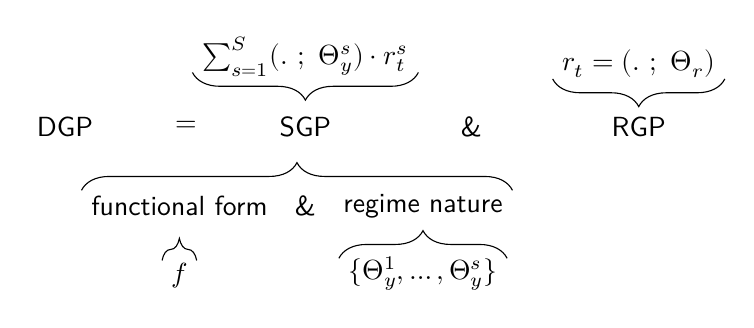
\begin{tikzpicture}[font=\sffamily]
% Styles:
\tikzset{mybrace/.style={decorate, decoration={brace, amplitude=10pt, raise=1.3ex}}}
\tikzset{node distance = 0.25cm and 0.1cm}

% Main nodes:
\node[] (dgp) {DGP};
\node[] (e)   [right = 0.8cm of dgp] {$=$};
\node[] (sgp) [right = 0.8cm of e] {SGP};
\node[] (p)   [right = 1.4cm of sgp] {\&};
\node[] (rgp) [right = 1.4cm of p] {RGP};

% Lower nodes:
\node[] (p2)   [below = 0.5cm of sgp] {\&};
\node[] (csgp) [left  = of p2] {functional form};
\node[] (rsch) [right = of p2] {regime nature};

% Math:
\node[] (msgp)  [above = of sgp] {$\sum_{s = 1}^S \sgp(. ~;~ \Theta_y^s) \cdot r_t^s$};
\node[] (mrgp)  [above = of rgp] {$r_t = \rgp(. ~;~ \Theta_r)$};
\node[] (mcsgp) [below = 0.35cm of csgp] {$f_{\sgp}$};
\node[] (mrsch) [below = of rsch] {$\{\Theta^1_y, \dots, \Theta^s_y\}$};

% Braces using the defined style, add mirror in place:
\draw[mybrace]         (csgp.west) -- (rsch.east);
\draw[mybrace, decoration={mirror}] (mrgp.west) -- (mrgp.east);
\draw[mybrace, decoration={mirror}] (msgp.west) -- (msgp.east);
\draw[mybrace, decoration={amplitude=8pt}]         (mcsgp.west) -- (mcsgp.east);
\draw[mybrace]         (mrsch.west) -- (mrsch.east);
\end{tikzpicture}

}

\end{figure}%

To construct a diverse set of DGPs, I combine different RGPs, SGPs, and
regime natures. One of the challenges of this work is to choose a
comprehensible set of these elements, and analyze their differences in a
systematic but manageable way.

In the notation above I omitted the error term inside \(f_{\sgp}\). Many
distributions are relevant, including fat-tailed and skewed ones. The
parameters \(\Theta_y\) can even encode different error distributions
across regimes. By imposing the same distribution across regimes, with
the possible exception of a multiplicative factor, the notation and
implementation is simplified. I then write the DGP as a function that
receives a sequence of random errors and returns the series and regimes:

\begin{equation}
    (y_{1:T},~ r_{1:T}) = \dgp(\varepsilon_{1:T};~ \Theta_r, \Theta_y)
\end{equation}

Consider the notation shorthand \(y \coloneqq y_{1:T}\), and similarly
for other variables, throughout the rest of this work.

Let the set of considered DGPs by \(P\) (for `processes'). These appear
in the literature, as discussed in Section~\ref{sec-lit}, and I define
them in Section~\ref{sec-impl}.

\subsection{Models}\label{sec-theory-models}

Consider a model \(\mod\) as a function with (hyper-) parameters
\(\Theta_m\) that generates fitted values and \(H\)-step-ahead
predictions of the series and regimes. The model can also return a set
\(\hat{\pi}\) of metadata, e.g.~the estimated coefficients.

\begin{equation}
    (\hat{y},~ \hat{r},~ \hat{\pi}) = \mod(y_{1:(T-H)} ~;~ \Theta_m)
\end{equation}

Notably, the number of estimated regimes \(\hat{S}\) is a parameter in
\(\Theta_m\), which may or may not be equal to \(S\). Let the set of
models be \(M\) (for `models'). Also present in the literature, they
will be defined in Section~\ref{sec-impl-sgp}.

\subsection{Regime-conditional metrics}\label{sec-theory-metrics}

A regime-conditional (RC) metric \(\met\) is a function that takes a
series and regimes, and returns a sequence with one value for each
regime. I use these metrics to characterize the distribution of \(y_t\)
and \((y_t, y_{t-j})\) within each regime.

\begin{equation}
    \met: (y, r) \mapsto \mathbb{R}^{S}
\end{equation}

An example is the function that returns, for each regime \(s\), the mean
of the series weighted by \(r^s_t\). This can be done for many common
metrics, and is equivalent to mapping \((y, r)\) to the \(S\) sets
\(R_s\) of regimes' observations,\footnote{\(R_s \coloneqq \{ y_t ~:~ r^s_t = \max\{r_t\} \}\).}
then applying the metric to each set. The benefit of the first approach
is that it is more general, allowing for non-binary -- i.e., smooth
transition -- regimes.

For the joint distribution \((y_t, y_{t-j})\), the metrics are more
complex, as they must consider only the windows
\((y_t, \dots, y_{t-j})\) fully contained in the same regime instance.
This is further described in Appendix~\ref{sec-app-metrics}.

In any case, RC metrics can pool observations from different time
windows. To interpret them as regime-specific distributions, I require
the series to be stationary within each regime. This requirement
restricts the DGPs that this work considers.

\subsubsection{Within-regime
stationarity}\label{within-regime-stationarity}

For the distribution of a regime to be well defined, all datapoints
within it must be drawn from the same distribution. Formally,
\emph{within-regime strong stationarity} requires, for all regimes
\(s \in S\), a CDF \(F_s\) such that:

\begin{equation}
\begin{array}{cc}
    F_s(y_{t_1}, \dots y_{t_n}) = F_s(y_{t_1+j}, \dots y_{t_n+j})  & 
    \begin{array}{c}
        \forall \{y_{t_1}, \dots y_{t_n}\}, \{y_{t_1+j}, \dots y_{t_n+j}\} \subset R_s, \\
        \forall j \in \mathbb{N}_*
    \end{array}
\end{array}
\end{equation}

As I characterize the distributions with specific metrics, weaker
assumptions can be made. Restricting attention to moments of the (joint)
distribution, I can impose the weak version. Formally,
\emph{within-regime weak stationarity} requires,\footnote{The ACF
  condition should be read as ``\(j\)'th autocorrelations between
  time-points within the same regime instance should always be equal'',
  not as ``\(j\)'th autocorrelations of every time-point in the same
  regime instance should always be equal'', although the latter is true
  for AR processes with order higher than \(j\).} for all \(s \in S\),
that:

\begin{equation}
\begin{array}{cc}
    E[y_t] = E[y_{t'}] & \forall y_t, y_{t'} \in R_s \\
    Var[y_t] = Var[y_{t'}] & \forall y_t, y_{t'} \in R_s \\
    Cov[y_t, y_{t-j}] = Cov[y_{t'}, y_{t'-j}] & 
    \begin{array}{c}
        \forall \{y_t, \dots, y_{t-j}\}, \{y_{t'}, \dots, y_{t'-j}\} \subset R_s, \\
        \forall j \in \mathbb{N}_*
    \end{array}
\end{array}
\end{equation}

Processes with non-binary \(r_t\), i.e., smooth transitions, do not have
truly separated regimes and therefore generally do not satisfy the
conditions above. In these cases, the metrics cannot be interpreted as,
for example, ``the mean of all observations in a regime''. Still, their
information may be useful, as I study in this work.

\subsubsection{Aspects of RC metrics usage}\label{sec-theory-usage}

There are two important aspects of the RC metrics usage. First is
whether to use the whole sequence of values for each \(s\), or to
condense it into a single value of dispersion across regimes. An example
of the latter is the `average pairwise distance between the RC means', a
single value that describes how distant the levels of the regimes are.
This is equivalent to composing a dispersion function \(\disp\):

\begin{equation}
    \disp \circ \met: (y, r) \mapsto \mathbb{R}^{S} \mapsto \mathbb{R}
\end{equation}

Second, which series to use: the true or estimated ones. One can use the
true values \((y, r)\) to get the characteristics of the true DGP, and
the estimated values \((\hat{y}, \hat{r})\) or \((y, \hat{r})\) to get
the characteristics of the estimated model.\footnote{Note that the value
  of \(S\) and \(\hat{S}\) can be different, and thus, so the dimension
  of the metric's output.} Another option is to calculate the difference
between the former and the latter.\footnote{This is only possible if
  \(S = \hat{S}\) and there is an unambiguous way to match the estimated
  and true regimes.} Another option is to calculate the metric of the
difference \((y - \hat{y}, r)\) or \((y - \hat{y}, \hat{r})\).

Less generally, sometimes there are other possible estimators for the
same population RC metric, rather than using \((\hat{y}, \hat{r})\)
directly. A special case arises when the metric is a moment of the
(joint) distribution and the SGP is simple: one can plug the estimated
parameters into the analytical formula for the moment and obtain a
better estimator. This is further discussed in
Appendix~\ref{sec-app-metrics}.

These options can be mixed-and-matched, depending on the question of
interest. In this work, I use estimated metrics computed from
\((y_{1:(T-H)}, \hat{r}_{1:(T-H)})\), as these are the values available
to the econometrician in practice, while I calculate the true metrics
analytically. I also ignore the regime-specific metric values and
instead condense them by considering only their dispersion, as this is
simpler and more comparable across DGPs and models.

Let the set of metrics \((\disp \circ \met)\) be \(C\) (for `criteria').
I define these in Section~\ref{sec-impl-metrics}, but they are mostly
based on moments of \(y_t\) and of the pair \((y_t, y_{t-j})\),
\(j \in \mathbb{N}\).

One can also describe the RGP using information such as each regime
instance's average duration, the transition probabilities, and measures
derived from them. I use these as control variables in the regression
analysis. Finally, regime-unconditional metrics can also be useful.

\section{Simulation framework}\label{sec-sim}

One goal of this work was to define the theoretical framework from the
previous section in a general and expandable way, so it can support
different exercises, including ones not considered here. I designed the
simulation structure with the same goal.

There are the following steps to perform the simulations:

\begin{enumerate}
\def\labelenumi{\arabic{enumi}.}
\tightlist
\item
  Generate random errors for all the DGPs.
\item
  For each DGP and simulation, generate the series and regimes,
  producing (\(y, r\)).
\item
  For each DGP and simulation, estimate each model, obtaining
  \((\hat{y},~ \hat{r})\).
\item
  For each DGP, simulation, and model, compute each metric.
\item
  Aggregate the metrics, performance information, and DGP and model
  descriptors into a dataset.
\end{enumerate}

\subsection{Hyperparameters}\label{sec-sim-hyper}

For the forecast performance, I focus on \(1\)-step ahead predictions.
It would be interesting to extend this, with or without
locally-projected models.

To obtain more than one prediction per simulation, I simulate a
\(T - H\)-long series and obtain \(H\) predictions. There are two
possible approaches:

\begin{enumerate}
\def\labelenumi{\arabic{enumi}.}
\tightlist
\item
  For each iteration \(h \in 1:H\), the model is estimated with the
  window \(h:(T-H+h-1)\), and generates \(\hat{y}_{T-H+h}\).
\item
  The model is estimated once with the window \(1:(T-H)\), then for each
  \(h\), \(\hat{y}_{T-H+h}\) is generated using \(y_{1:(T-H+h-1)}\).
\end{enumerate}

The second approach is computationally cheaper, allowing for more
simulations and DGPs to be considered. It is the one used in this work,
but note that it is less accurate to what would be done in practice, as
econometricians often re-estimate their models with new data.

Overall, the hyperparameters of the simulation are as follows:

\begin{itemize}
\tightlist
\item
  Number of simulations: \(I\). Its main effect is on the precision of
  the results, and diversity of series.
\item
  Forecast horizon: \(H\) predictions of \(1\)-step ahead values. It
  also affects the precision of the results, but does not change the
  diversity of series.
\item
  Total number of observations: \(T\). Its main effect is on the ability
  of the models to learn the dynamics and separate the regimes. Results
  for higher \(T\)'s are more relevant for contexts with a lot of data,
  such as high-frequency financial data, while lower \(T\)'s are more
  relevant for contexts with less data, such as macroeconomic data.
\item
  Burn-in period: \(B\). Its main effect is on reducing dependence on
  initial values, but with stationary processes this is not too
  problematic.
\end{itemize}

Let \(i \in 1:I\), \(I \in \mathbb{N}\) be the simulation index.

\subsection{Simulation algorithm}\label{simulation-algorithm}

I only consider DGPs with the same error distribution -- but note that a
DGP can still have a volatility parameter multiplying its error. For
each DGP, indexed by \(p \in 1:|P|\), there are \(I\) random error
vectors, each of size \(T\). Let \(\Epsilon\) denote the set of all
errors. Let \(\Epsilon_{p, i}\) denote the vector of errors generated
for the \(p\)-th DGP and the \(i\)-th simulation. Similar indexing
definitions are used for similar collections throughout this document.

Let \(Y\) and \(R\) denote the sets of generated series and regimes.
They are computed given \(\Epsilon_{p, i}\):

\begin{algorithm}[H]
\begin{algorithmic}[1]
    \State Initialize $Y$ and $R$
    \For{$p$ \textbf{in} $1:|P|$}
        \For{$i = 1$ \textbf{to} $I$}
            \State $Y_{p, i},~ R_{p, i} \gets P_p(\Epsilon_{p, i})$
    \EndFor
\EndFor
\end{algorithmic}
\end{algorithm}
\vspace{-0.5em}

Now, for each simulation, I estimate each model, generating the sets
\(\hat{Y}\), \(\hat{R}\), and \(\hat{\Pi}\). The models are trained
using only \(y_{(B+1):(T-H)}\), to avoid the burn-in period and leave
space for the forecast horizon. The nesting order is the same, but with
an additional inner loop for the model estimation.

\begin{algorithm}[H]
\begin{algorithmic}[1]
    \State Initialize $\hat{Y}$ and $\hat{R}$
    \For{$p$ \textbf{in} $1:|P|$}
        \For{$i$ \textbf{in} $1:I$}
            \For{$m$ \textbf{in} $1:|M|$}
                \State $\hat{Y}_{p, i, m},~ \hat{R}_{p, i, m},~ \hat{\Pi}_{p, i, m} \gets M_m(Y_{p, i},~ R_{p, i})$
            \EndFor
        \EndFor
    \EndFor
\end{algorithmic}
\end{algorithm}
\vspace{-0.5em}

Then, for each model, the dispersion of the RC metrics are calculated
and stored as columns of a dataset \(D\). Each row of \(D\) is
identified by \((p, i, m)\).

\begin{algorithm}[H]
\begin{algorithmic}[1]
    \State Initialize $D$
    \For{$(p, i, m)$ \textbf{in} $(1:|P|) \times (1:I) \times (1:|M|)$}
        \For{$c$ \textbf{in} $1:|C|$}
            \State $D_{(p, i, m),~ c} \gets C_c(Y_{p, i, m}, R_{p, i, m},~ \hat{Y}_{p, i, m},~ \hat{R}_{p, i, m})$
        \EndFor
        \State $\hat{\Pi}_{p, i, m}$ is appended to $D_{p, i, m}$.
        \State Categorical variables $(p, i, m)$ are appended to $D_{p, i, m}$.
    \EndFor
\end{algorithmic}
\end{algorithm}
\vspace{-0.5em}

Recall the discussion in Section~\ref{sec-theory-metrics} about the two
different aspects of RC metrics usage. With different options, the
function \(C_c\) can use different inputs (\(Y, R\), \(Y, \hat{R}\), or
\(\hat{Y}, \hat{R}\)), which is represented by all four objects being
passed to it. Additionally, the function could return the whole sequence
of RC metrics, not a single value, then, each row would be identified by
\((p, i, m, s)\). While the metrics receive the full dataset, estimation
is only done with \((B + 1):(T - H)\).

The dataset \(D\) is already in a friendly format for analyzing the
relationship between each observation's performance and the regimes'
characteristics, and for stratifying by DGP and model.

\section{Implementation}\label{sec-impl}

The framework described in the last two sections is general and
accommodates many exercises. In this work, I focus on a specific set of
DGPs, models, and metrics. I describe them here.

I focus on regime-switching DGPs with two regimes (\(S = 2\)). Studying
how well models identify regime dynamics with a different number of
regimes is an interesting extension. I also include a no-RS model as a
baseline.

I choose hyperparameters to balance the DGP `population'. I restrict the
SGP to a simple stationary \(AR(1)\) process. I consider
Markov-switching, Self-Exciting Threshold, and Smooth Transition RGPs,
each equally represented, with symmetric and asymmetric variants. For
each of the three \(AR(1)\) parameters, I consider two RNs: a `small'
and a `large' change. I choose the related hyperparameters guided by the
concept of `regime separation', described in Section~\ref{sec-sep}. I
also include two additional models: K-Means and Random Forest.

Model choice and hyperparametrization are more flexible because they do
not affect the experiments' `population'. I use each RGP's empirical
model counterpart with a `generic' hyperparametrization. Increasing
model diversity would be a useful extension.

I limit the metrics to essential descriptors of the regime
distributions: the first and second moments and the lag-1
autocorrelation. This set could be expanded. I also define performance
and RGP-related metrics for the regression analysis.

Finally, I discuss diagnostics for series generation and model
estimation and describe the final dataset.

\subsection{Considered SGPs}\label{sec-impl-sgp}

The SGP functional form may matter through its interaction with the
other ingredients of the DGP. Some applications require specific SGPs,
such as conditional volatility in finance and GARCH models. Here, this
is not the main point of interest. I therefore consider only an
\(AR(1)\) process for its simplicity, popularity, and ease of
estimation.

I also assume a Gaussian distribution for the error term, ignoring
fat-tailed and skewed alternatives. The distribution is
regime-invariant, except for the multiplicative variance parameter
\(\sigma\).

As discussed, I assume within-regime weak stationarity, even though many
interesting DGPs are non-stationary. This restricts the absolute value
of the \(AR(1)\) parameter to be less than \(1\). I consider only the
following SGP functional form:

\begin{equation}
\begin{array}{ll}
    &f_{\sgp}(. ~;~ (\mu^s, \rho^s_1, \sigma^s)) = \mu^s + \rho^s_1 y_{t-1} + \sigma^s \cdot \varepsilon_t\\
    &\varepsilon_t \sim \mathcal{N}(0, 1)\\
    &|\rho^s_1| < 1, ~~ \sigma^s > 0, ~~ \forall s \in 1:S
\end{array}
\end{equation}

Several other SGPs could be considered, including transformations of
\(y_t\) as regressors, nonlinear regression forms, or decision trees, as
in the common Markov-switching Random Forest model. The \(AR(1)\)
remains an essential building block, and its simplicity helps isolate
the effects of the other ingredients.

\subsection{Considered RGPs and models}\label{sec-impl-rgp}

The next ingredient is the RGP. I consider Self-Exciting Threshold,
Smooth Transition, and Markov-switching. I also include a no
regime-switching benchmark.{[}\^{}sb{]}

Each RGP has an empirical model counterpart, which I also consider.

The formal definition of each RGP/model is presented in
Appendix~\ref{sec-app-cons}, first the RGP hypothesis, then the
empirical model estimation strategy.

For each RGP, I consider a symmetric case with equally likely regimes
and an asymmetric variant.

\begin{itemize}
\tightlist
\item
  \textbf{No Regime Switching:}

  \begin{itemize}
  \tightlist
  \item
    Always in regime 1.
  \end{itemize}
\item
  \textbf{Self-Exciting Threshold:}

  \begin{itemize}
  \tightlist
  \item
    Fixed hyperparameters: switching based on \(y_{t-1}\). Different
    lags often reflect timing choices and are not considered here.
  \item
    A single threshold at \(0.5\), and a single threshold at \(0.9\).
  \end{itemize}
\item
  \textbf{Smooth Transition:}

  \begin{itemize}
  \tightlist
  \item
    Fixed hyperparameters: switching based on \(y_{t-1}\), the logistic
    CDF as transition function.
  \item
    A single threshold at \(0.5\), and a single threshold at \(0.9\).
  \end{itemize}
\item
  \textbf{Markov-switching:}

  \begin{itemize}
  \tightlist
  \item
    Symmetric matrix, high persistence (\(P(s | s) = 0.9\)).
  \item
    Asymmetric matrix, high persistence (\(P(1 | 1) = 0.9\),
    \(P(1 | 2) = 0.3\)).
  \end{itemize}
\end{itemize}

I considered a structural-break model, but analyses suggested it behaved
differently from the other models because it does not generate recurring
regimes, as expected. I therefore dropped it from the final set of
models.

I choose values to target a \(50\%\) proportion of regime 1 in the
symmetric case and \(75\%\) in the asymmetric case for each DGP. The
Table~\ref{tbl-regimes_sim} shows the absolute deviation of the regime 1
proportion from 0.5; I target values close to 0 for the symmetric case,
and close to 0.25 for the asymmetric case. RGP and RN interact, so the
same RGP can yield different regime proportions across RNs.

\begin{table}[!htbp]

\caption{\label{tbl-regimes_sim}Proportion of regimes across DGPs}

\centering{

\begin{tabular}{@{\extracolsep{\fill}}l|rrrrrrr}
\toprule
 & Uncond. & \(\mu ~ (0, 0.5)\) & \(\mu ~ (0, 1)\) & \(\rho_{1} ~ (0.1, 0.9)\) & \(\rho_{1} ~ (0.4, 0.6)\) & \(\sigma ~ (1, 1.5)\) & \(\sigma ~ (1, 2)\) \\ 
\midrule\addlinespace[2.5pt]
No RS & .50 & .50 & .50 & .50 & .50 & .50 & .50 \\ 
MS, \(p_{21} = 0.1\) & .02 & .03 & .02 & .03 & .02 & .03 & .02 \\ 
MS, \(p_{21} = 0.3\) & .23 & .24 & .23 & .23 & .23 & .24 & .23 \\ 
SET, \(\tau = 0.5\) & .12 & 00 & .24 & .12 & .01 & .18 & .19 \\ 
SET, \(\tau = 0.9\) & .19 & .18 & .04 & .25 & .15 & .28 & .27 \\ 
ST, \(\tau = 0.5\) & .13 & 00 & .13 & .19 & .25 & .11 & .08 \\ 
ST, \(\tau = 0.9\) & .19 & .12 & .02 & .30 & .34 & .21 & .16 \\ 
\bottomrule
\end{tabular}


}

\end{table}%

Two additional models, with no RGP counterpart, are considered: Random
Forest and K-Means clustering. Both receive four lags of the series, and
the rolling average, ACF(1), and SD of the series. The RF does not
generate a regime series, and is included as benchmark in only some of
the analyses. The RF uses 50 trees and 10 minimum terminal node size.

The K-Means is and interesting model because it does not rely on a
specific assumption on the RGP structure. The Random Forest is
interesting because, while it does not directly model the states, the
brancing structure of decision trees can capture regime-like dynamics.

For the models, most hyperparameters are as follows:

\begin{itemize}
\tightlist
\item
  I allow all coefficients to change across regimes; this is a common
  assumption, particularly under possible mis-specification.
\item
  I fix the number of regimes \(\hat{S}\) rather than estimate it.
  Models are estimated with 2 regimes.
\item
  Model-specific hyperparameters match the related RGP values.
\end{itemize}

\subsection{Considered regime natures}\label{sec-impl-rn}

The following regime natures are considered, each representing a
different way in which the SGP parameters change across regimes:

\begin{itemize}
\tightlist
\item
  \textbf{Mean (\(\mu\)) change:}

  \begin{itemize}
  \tightlist
  \item
    Small difference: (\(\mu^1 = 0\), \(\mu^2 = 0.5\))
  \item
    Large difference: (\(\mu^1 = 0\), \(\mu^2 = 1\))
  \end{itemize}
\item
  \textbf{Persistence (\(\rho_1\)) change:}

  \begin{itemize}
  \tightlist
  \item
    Small difference: (\(\rho_1^1 = 0.4\), \(\rho_1^2 = 0.6\))
  \item
    Large difference: (\(\rho_1^1 = 0.2\), \(\rho_1^2 = 0.8\))
  \end{itemize}
\item
  \textbf{Volatility (\(\sigma\)) change:}

  \begin{itemize}
  \tightlist
  \item
    Small difference: (\(\sigma^1 = 1\), \(\sigma^2 = 1.5\))
  \item
    Large difference: (\(\sigma^1 = 1\), \(\sigma^2 = 2\))
  \end{itemize}
\end{itemize}

I order regimes by increasing value of the parameter of interest. In the
asymmetric RGPs, the rarer regime is always the second one, with the
higher value of the relevant parameter.

I choose values to match the regimes' proportion discussed in the last
section, and to generate a reasonable level of regime separation, as
described in Section~\ref{sec-sep}.

\subsection{Considered metrics}\label{sec-impl-metrics}

The goal with RC metrics is to capture changes in the series'
characteristics across regimes. One important option is the estimated
parameters of the model for each regime, e.g.,
\((\hat{\rho}_s)_{s \in \hat{S}}\), \((\hat{\mu}_s)_{s \in \hat{S}}\),
etc. One might expect these to outshine all other metrics, but in more
complex cases where more than one parameter changes, this becomes less
useful. More general metrics benefit from their abstraction over the
DGP. Additionally, in simple SGPs, there often is a metric that is
directly connected to changes in parameters, such as the conditional
average for changes in intercept.

In this work, I focus on the moments of the distribution of \(y_t\) and
\((y_t, y_{t-j})\). Specifically, the RC metrics considered are the RC
mean, RC standard deviation, and RC autocorrelation of lag 1. Higher
lags could be considered, but in the simple \(AR(1)\) context this would
add little additional information.

As stated before, the RC mean and RC SD are simply the mean and SD of
each set \(R_s\). The autocorrelation is similar, but must be calculated
separately for each concurrent set of observations in \(R_s\). The
formal definitions are stated in the Appendix~\ref{sec-app-metrics}.

Because the focus is on the dispersion of RC metrics, two important
measures to consider are the standard deviation and the average pairwise
absolute difference. For only two regimes, they are very similar and the
absolute difference is more intuitive. I define the metrics so that all
\(\disp \circ \met \in C\) return a single real value, and
\(\disp(x) = |x_1 - x_2|\).

There are some possible expansions on this work's metrics calculation.
One is to use non-standard weights for the empirical moments, giving
more importance to observations near the edges of regimes' instances.
Another is to use a cluster separation measure, such as the silhouette
score, instead of a simple absolute distance between the RC metrics.
Finally, one can use distribution distance metrics. These are not
currently considered. No regime-unconditional metrics are considered.
The list of considered metrics is as below:

\begin{itemize}
\tightlist
\item
  First moment: RC mean \(\hat{\mu}(y | S)\).
\item
  Second moment: RC standard deviation \(\hat{\sigma}(y | S)\).
\item
  First autocorrelation: RC lag-1 autocorrelation
  \(\hat{\rho_1}(y | S)\).
\end{itemize}

\subsubsection{Performance and RGP
metrics}\label{performance-and-rgp-metrics}

The performance metrics considered are the RMSE for forecasting
performance. The MSE is not included, following Dacco; Satchell (1999).
The fit performance is measured by \(R^2\) for \(y\) and binary mean
error for \(r\).

I also include RGP-related metrics in the regression analysis: the
number of regime switches divided by \(T\), as a measure of switching
frequency; the absolute difference between the average duration of
regime 1 instances and regime 2 instances, as a measure of regime
asymmetry.

For works with more than two regimes, more complex measures of regime
asymmetry can be used, ones that consider the whole matrix of transition
probabilities.

\subsection{Simulation and diagnostics}\label{sec-impl-diag}

I implement the simulations and analyze them in the next sections using
the R programming language, and the code can be found in
\href{https://github.com/ricardo-semiao/article-regime-id-performance}{this
paper's repository}. The code is highly modular and fully reproducible,
following the intent of setting up an expandable framework.

Following Section~\ref{sec-sim-hyper}, the chosen hyperparameters are as
below. Some values are lower than they could be due to computational
constraints. The choice of \(T\) is discussed in
Section~\ref{sec-sep-across}.

\begin{itemize}
\tightlist
\item
  Number of simulations: \(I = 500\).
\item
  Forecast horizon: \(H = 10\) predictions of \(1\)-step ahead values.
\item
  Total number of observations: \(T = 100\).
\item
  Burn-in period: \(B = 4\).
\item
  As described above, there are \(6\) RNs, \(7\) RGPs, and \(4\) models.
\end{itemize}

I generate the error sequences in parallel, using
\href{https://github.com/cran/rTRNG}{\texttt{rTRNG::rnorm\_trng}}. I
estimate the models with
\href{https://github.com/SurajGupta/r-source/tree/master/src/library/stats}{\texttt{stats::lm}},
\href{https://github.com/cran/mbreaks}{\texttt{mbreaks::dofix}},
\href{https://github.com/cran/tsDyn}{\texttt{tsDyn::setar}},
\href{https://github.com/cran/tsDyn}{\texttt{tsDyn::lstar}},
\href{https://github.com/cran/MSwM}{\texttt{MSwM::msmFit}}, and
\href{https://github.com/cran/randomforest}{\texttt{randomforest::randomForest}}.

Beyond visualizing the series and guaranteeing no missing values, I
perform diagnostics on the simulation, model estimation, and metrics
calculation. All of the diagnostics are presented in
Appendix~\ref{sec-app-diag}.

The errors should be i.i.d. Gaussian with mean \(0\) and should not
present any pattern, especially across the parallelization structure.
This is guaranteed by the TRNG library, but I also check it.

Some observations had to be removed. Table~\ref{tbl-estimation_issues}
lists the reasons and the amounts; some observations have multiple
issues, which explains the difference between the `\% Bad' and `\%
Removed' columns. Some models did not converge and produced no output.
Others could not estimate some parameters. The need to remove those is
straightforward.

Some models' predictions were dominated by one regime and produced zero
or only one observation of the other. While this is not a failed
estimation, calculating the dispersion of regimes' distributions is
impossible in these cases, and they would be removed from most analyses
anyway. Appendix~\ref{sec-app-diag-r} plots the distribution of regimes'
proportions, and notably, K-Means has the most balanced regimes.

The last removal is less straightforward. Some models generated
unreasonably large errors, and parameters unreasonably outside the
normal range, so they would commonly be disregarded. This is more
subjective and prone to cherry-picking; thus I was parsimonious in this
removal. Only RMSEs higher than 50, means higher than the 90th quantile
of the whole dataset, and \(\rho_1\)s higher than 10 standard deviations
of all the \(\rho_1\) estimates were removed.

Appendix~\ref{sec-app-diag-error} shows the distribution of fits and
RMSEs. Notably, the RF shows signs of overfitting, because the chosen
generic hyperparameterization is overkill for the simple SGPs
considered. Appendix~\ref{sec-app-diag-params} shows the distribution of
the estimated \(AR\) parameters; ST has distributions with more
variance. It also shows distributions of other model parameters. The RF
feature importance ranks the first two lags and the rolling average as
most important, while the ACF and SD have much lower importance.

\begin{table}[!htbp]

\caption{\label{tbl-estimation_issues}Estimation issues}

\centering{

\begin{tabular}{@{\extracolsep{\fill}}l|rrrr}
\toprule
 & Bad obs. & \% Bad & \% Removed & Obs. left \\ 
\midrule\addlinespace[2.5pt]
Full sample & 0 & 0\% & 0\% & 126,000 \\ 
Bad convergence & 148 & 0.1\% & 0.1\% & 125,852 \\ 
NAs in parameters & 245 & 0.2\% & 0.2\% & 125,607 \\ 
Low \#obs. in regimes & 967 & 0.8\% & 0.6\% & 124,859 \\ 
Unreasonable parameters & 1,803 & 1.4\% & 1.3\% & 123,162 \\ 
Unreasonable errors & 145 & 0.1\% & 0\% & 123,137 \\ 
{\bfseries Total} & {\bfseries 3,308} & {\bfseries 2.6\%} & {\bfseries 2.3\%} & {\bfseries 123,137} \\ 
\bottomrule
\end{tabular}


}

\end{table}%

The average coefficient generated by the models is presented in
Appendix~\ref{sec-app-diag-params}. Only the matched model-RGP pairs are
included, and a test of difference against the true parameter is
performed. Many tests don't pass, but that is expected, as all
parameters are allowed to change across regimes. It is important to note
that they generally do (except for \(\sigma\)).

To consider the metrics estimation, the regime-conditional and
unconditional moments are estimated using and tested against their true
values in Appendix~\ref{sec-app-diag-metrics}. The estimations use
\((y, r)\), while the true values are calculated via the analytical
formula (the unconditional true values are not calculated). Again, the
tests are not generally expected to pass, especially given their high
power.

As a final placebo test, the forecast performance (RMSE) was regressed
against the index \(i\) of the simulation. The
Table~\ref{tbl-i_independence} shows generally no relation, as expected.

\section{Regimes' distribution}\label{sec-sep}

In this section, I explore what the regimes' distributions, as captured
by the RC metrics, reveal about regime DGPs and models. This helps
interpret the systematic results of the next section and provides
stylized facts for the econometrician.

The first two subsections, \ref{sec-sep-in} and \ref{sec-sep-across},
summarize, for each DGP, regime separation under each metric, first for
the full sample and then as sample size varies.
Section~\ref{sec-sep-models} examines how the models capture that
separation.

\subsection{\texorpdfstring{Regime separation in
\(T\)}{Regime separation in T}}\label{sec-sep-in}

I first ask what each DGP implies for the distribution of \(y_t\) across
regimes. One could plot regime-conditional distributions (and, ideally,
the joint distribution of \((y_t, y_{t-1})\)), but these visualizations
become difficult to interpret when repeated across many DGPs and
hyperparameter settings.

The approach in this work is instead to characterize each regime
distribution with regime-conditional metrics, and to summarize ``how
different the regimes are'' by a dispersion across regimes. As stated
before, more metrics than the ones considered here could be necessary to
fully capture the differences between regimes.

Consider Table~\ref{tbl-metrics_sep_t}. It should be read as a compact
`profile' of the DGP in terms of regime separation. Each \emph{row}
corresponds to one DGP configuration, grouped by the regime-generating
process (RGP) and the regime-nature parameter (RN); for each RC metric
(mean, lag-1 autocorrelation, and standard deviation), there are two
\emph{columns} corresponding to the RN's `small' and `big' parameter
changes; each \emph{cell} reports the absolute difference in the
corresponding RC metric across the two regimes, as well as the `(SD)'
and non-zero-test p-value stars. The table uses only symmetric RGPs, as
well as 100 of the simulation indices. The metrics are calculated with
\((y, r)\).

\begin{table}[!htbp]

\caption{\label{tbl-metrics_sep_t}Regimes' metrics separation across
DGPs}

\centering{

\begin{table}[t]
\fontsize{12.0pt}{14.0pt}\selectfont
\begin{tabular*}{\linewidth}{@{\extracolsep{\fill}}l|l|cccccc}
\toprule
\multicolumn{2}{l}{} & \multicolumn{2}{c}{{\(d(\hat{\mu}(.))\)}} & \multicolumn{2}{c}{{\(d(\hat{\rho}_1(.))\)}} & \multicolumn{2}{c}{{\(d(\hat{\sigma}(.))\)}} \\ 
\cmidrule(lr){3-4} \cmidrule(lr){5-6} \cmidrule(lr){7-8}
RGP & Param. \textbackslash{} RN & \((0, 0.5)\) & \((0, 1)\) & \((0.1, 0.9)\) & \((0.4, 0.6)\) & \((1, 1.5)\) & \((1, 2)\) \\ 
\midrule\addlinespace[2.5pt]
MS & \(\mu\) & .74 (.01)*** & 1.54 (.05)*** & .01 (0) & .02 (.05) & .04 (0) & .07 (.01) \\ 
 & \(\rho_{1}\) & .04 (.05) & .13 (.26) & .17 (.05)*** & .31 (.04)*** & .11 (0)** & .45 (.14)*** \\ 
 & \(\sigma\) & .1 (.11) & .11 (.27) & .03 (.03) & .01 (.03) & .55 (.01)*** & 1.08 (.12)*** \\ 
SET & \(\mu\) & 1.55 (.11)*** & 2.22 (.23)*** & .03 (.01) & .2 (.04)*** & .03 (.06) & 0 (.11) \\ 
 & \(\rho_{1}\) & .94 (.05)*** & 1.29 (.23)*** & .01 (.01) & .17 (.05)*** & .02 (.07) & .17 (.1)*** \\ 
 & \(\sigma\) & 1.13 (.16)*** & 1.12 (.26)*** & .11 (.06)*** & .11 (.09)** & .48 (.09)*** & 1 (.11)*** \\ 
ST & \(\mu\) & .62 (.04)*** & .39 (.02)*** & .03 (.04) & .12 (.01)*** & .04 (.01) & .01 (0) \\ 
 & \(\rho_{1}\) & .88 (.03)*** & 1.12 (.07)*** & .22 (.04)*** & .43 (.02)*** & .15 (.03)*** & .26 (.01)*** \\ 
 & \(\sigma\) & 1.18 (.1)*** & 1.38 (.06)*** & .13 (.06)*** & .02 (0) & .29 (.01)*** & .49 (.12)*** \\ 
\bottomrule
\end{tabular*}
\end{table}



}

\end{table}%

In the first row (MS with a \(\mu\) change), only the mean separates the
regimes, as expected. With a change in \(\rho_1\), both the ACF and the
SD differentiate the regimes, because the standard deviation depends on
\(\rho_1\). When \(\sigma\) changes, only SD differentiates the regimes.
This suggests a mapping from which metric differentiates the regimes to
which parameter changes in the DGP, but this mapping is not universal,
because it changes as we consider other RGPs.

MS has the cleanest result because its RGP does not depend directly on
\(y\), so it interacts less with the RN. For (SET, \(\mu\)), the mean is
separated, but the (big) ACF and SD also separate. This happens because
in the `big' regime, a higher mean creates a feedback loop that keeps
values higher. With a \(\rho_1\) change, the mean also increases: in the
`big' regime, higher \(\rho_1\) amplifies large values, raising the
mean. For \(\sigma\), a similar effect occurs: the `big' regime has
larger variation and larger maxima, while the `small' regime has smaller
variation and smaller minima, increasing the mean difference across
regimes.

With ST, we obtain a similar result, as its RGP is very similar to SET.
Notably, ST shows higher separation in the `small' RNs, which SET does
not show as clearly. Overall, this table exemplifies the importance of
the RGP--RN interaction. This is relevant for understanding models'
performance and how metrics' profiles vary with it.

\subsection{\texorpdfstring{Regime separation across
\(t\)}{Regime separation across t}}\label{sec-sep-across}

It is intuitive that sample size affects whether estimated metrics
detect separation across regimes. The ability to learn regime dynamics
depends not only on which parameter changes (RN), but also on how
quickly the induced regime separation becomes statistically visible as
\(T\) increases. To study the interaction between RGP, RN and \(T\), I
calculate each metric with the data up to each time point (\(1:2\),
\(1:3\), \(\dots\), \(1:T\)). By graphing the last time point considered
on the x-axis and the across-regime difference of the RC metric on the
y-axis, we can see how separation evolves with sample size.

The figures \ref{fig-rs-ms} - \ref{fig-rs-st} present the results. The
x-axis is the last time point included in the `effective sample', used
to calculate the line and ribbon at that value; each line is the average
(across simulations) of the metrics' dispersion, and the ribbon is
calculated as the standard error (across simulations) times 1.96. Both
are stratified by RGP symmetry, indicated via color. The graphs use only
the big RNs, and 20 simulation indices. The metrics are calculated with
\((y, r)\).

Two main results emerge. First, asymmetry mainly affects uncertainty:
average values across asymmetric and symmetric cases are very similar,
but the standard deviation is not. This is because the less frequent
regime contributes few observations, and this number grows very slowly
across time.

Second, the values and their standard deviations seem to be more or less
stabilized around \(T = 60\), which means that for a series of this size
(60 to 100 observations) we would likely see similar usefulness of these
metrics. For smaller series, the metrics are substantially less
informative.

\begin{figure}

\caption{\label{fig-rs-ms}Regime separation - MS}

\centering{

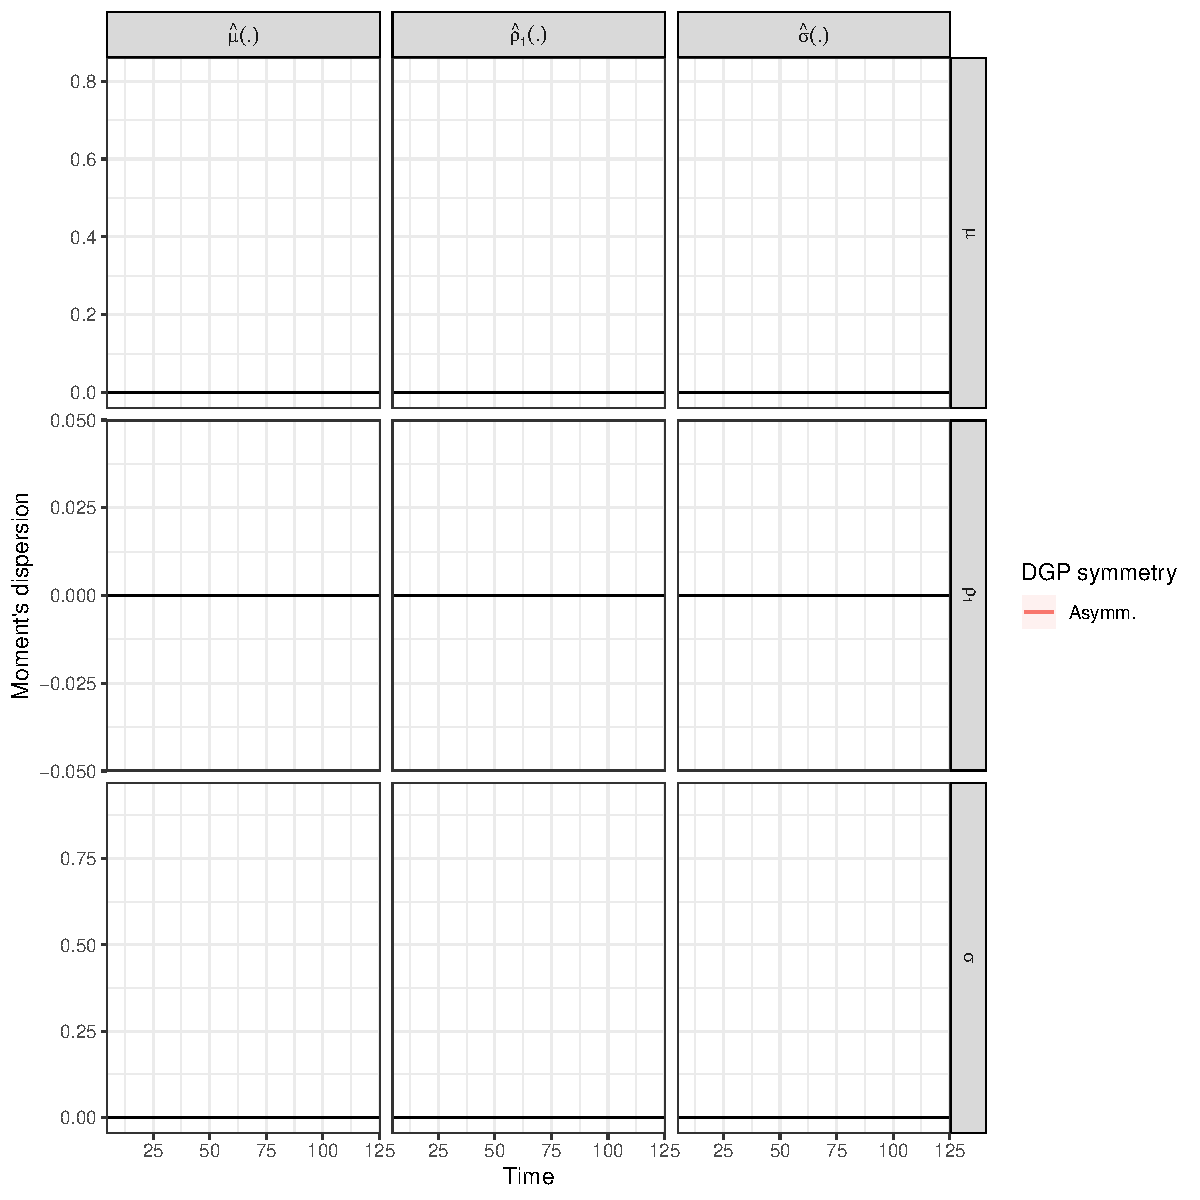
\includegraphics[width=\linewidth,height=0.4\textheight,keepaspectratio]{../../outputs/exploratory/metrics_sep_ms.pdf}

}

\end{figure}%

\begin{figure}

\caption{\label{fig-rs-set}Regime separation - SET}

\centering{

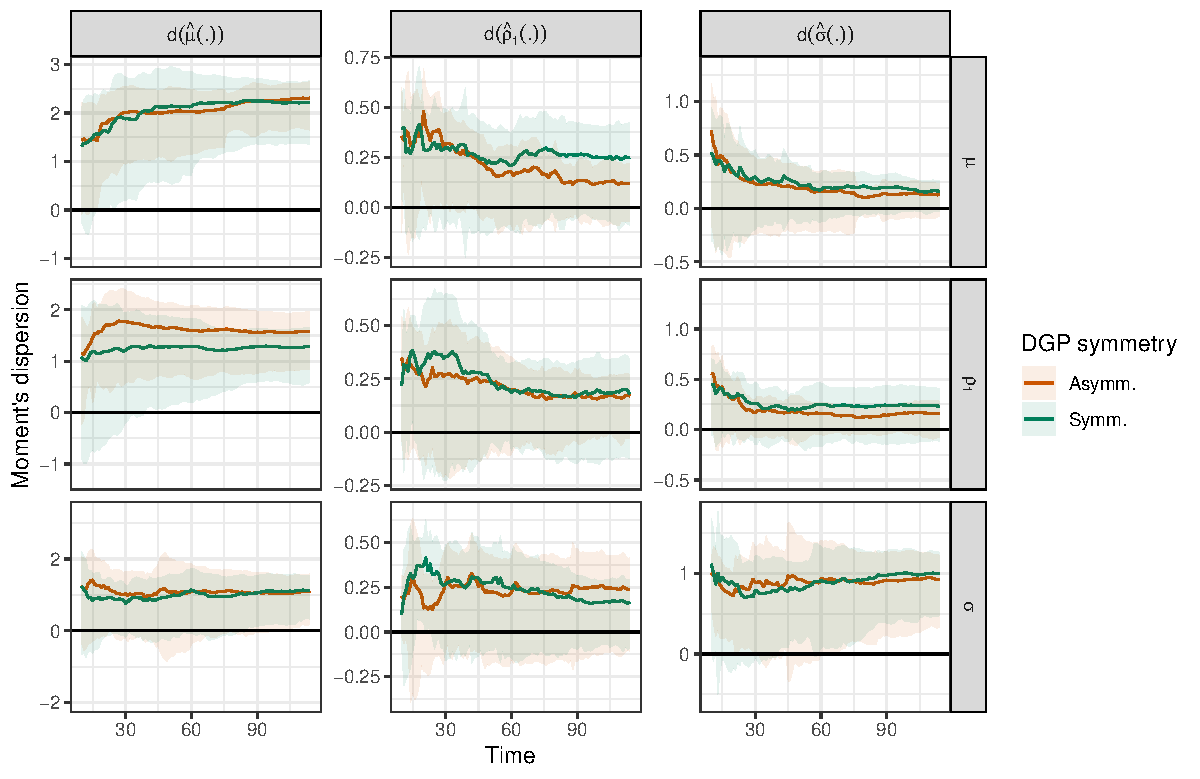
\includegraphics[width=\linewidth,height=0.4\textheight,keepaspectratio]{../../outputs/exploratory/metrics_sep_set.pdf}

}

\end{figure}%

\begin{figure}

\caption{\label{fig-rs-st}Regime separation - ST}

\centering{

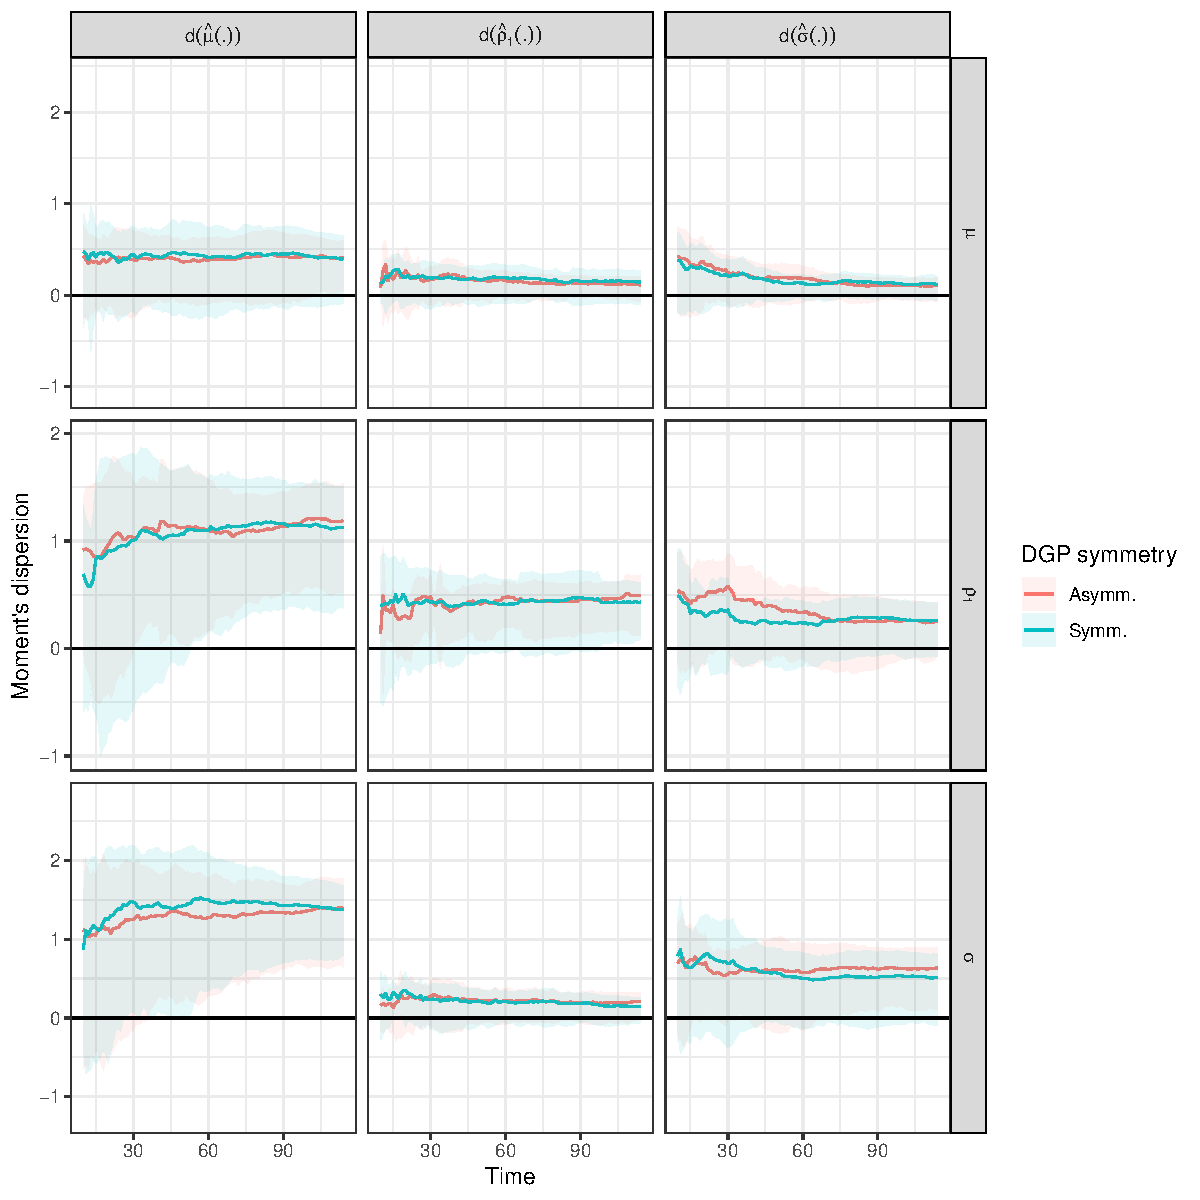
\includegraphics[width=\linewidth,height=0.4\textheight,keepaspectratio]{../../outputs/exploratory/metrics_sep_st.pdf}

}

\end{figure}%

\subsection{Models and regimes}\label{sec-sep-models}

To study how the models' estimates relate to regime separation, I
compare the estimated metrics with the true ones. I do this in
Figure~\ref{fig-metrics_diff}, which shows the absolute difference
between the true and estimated dispersion of the RC metrics. Each panel
row corresponds to a parameter change, and each panel column to a
metric. The estimated metrics are calculated with \((y, \hat{r})\),
while the true metrics are calculated via the analytical formula; thus,
this difference combines metric-estimation error and \(\hat{r}\) error.
The metrics were scaled by their median absolute difference (MAD) for
comparability.

\begin{figure}[!htbp]

\caption{\label{fig-metrics_diff}Metrics difference}

\centering{

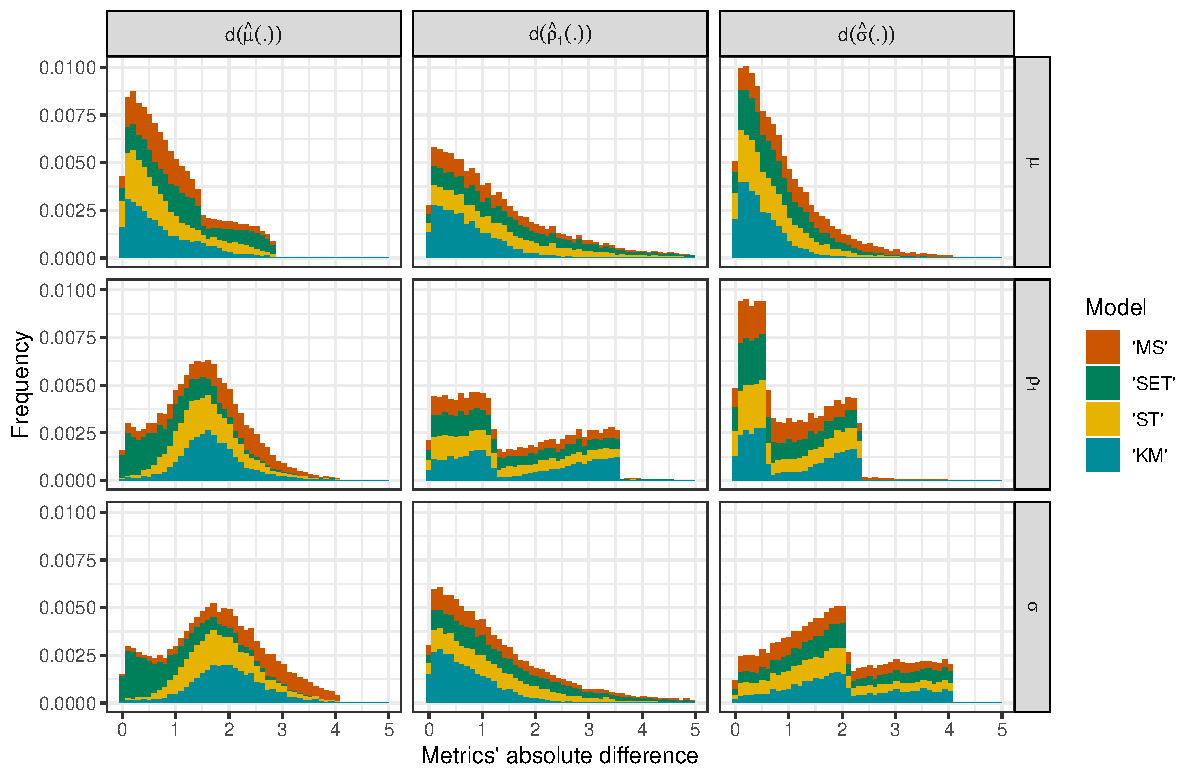
\includegraphics[width=\linewidth,height=0.4\textheight,keepaspectratio]{../../outputs/exploratory/metrics_diff.pdf}

}

\end{figure}%

We can see that KM and ST do well with the mean when \(\mu\) is
changing, but not otherwise, while SET has a more balanced result, and
MS performs worst. KM overall shines with \(\mu\) changes, possibly
because it includes four lags of the series level in its composition.
More importantly, the distribution for any given metric varies widely
across RNs. This means that no model makes a `fixed' error for each
metric: depending on the unobservable RN, the correctness of the
estimated metrics varies. In contrast, a graph stratified by RGP would
show that each metric error is somewhat invariant across RGPs. This will
be relevant in Section~\ref{sec-perf-mis}. The breaks in the
distributions come from the fact that the true metrics are set values
for each DGP.

Another useful analysis relates model outputs (estimated fit, \(r\),
parameters) to model performance. The fit and parameters, continuous
variables, are studied in Section~\ref{sec-perf-id}. The binarized
regime assignment has special importance, as it is directly related to
regime separation, and can be used to split the forecasting errors into
``correctly identified'' and ``incorrectly identified'' observations.
The figures \ref{fig-rp-nors} - \ref{fig-rp-st} compare the distribution
of individual forecasting errors, conditional on whether the underlying
regime was correctly identified. Each panel corresponds to a DGP
configuration and presents the distribution of forecasting errors
stratified by regime correctness; each figure corresponds to one model.
The graphs are done with big RNs, symmetric RGPs, and 100 simulation
indices.

In general terms, the `correct' distributions have slimmer tails, which
is in line with the literature. This is not always the case, however,
especially for the MS model; this result will be discussed in
Section~\ref{sec-perf-fe}. For the ST model with no-RS RGP, we have high
errors overall and bimodal distributions, which will be discussed in
Section~\ref{sec-perf-mis}.

\begin{figure}

\caption{\label{fig-rp-nors}Regime and series prediction - no-RS}

\centering{

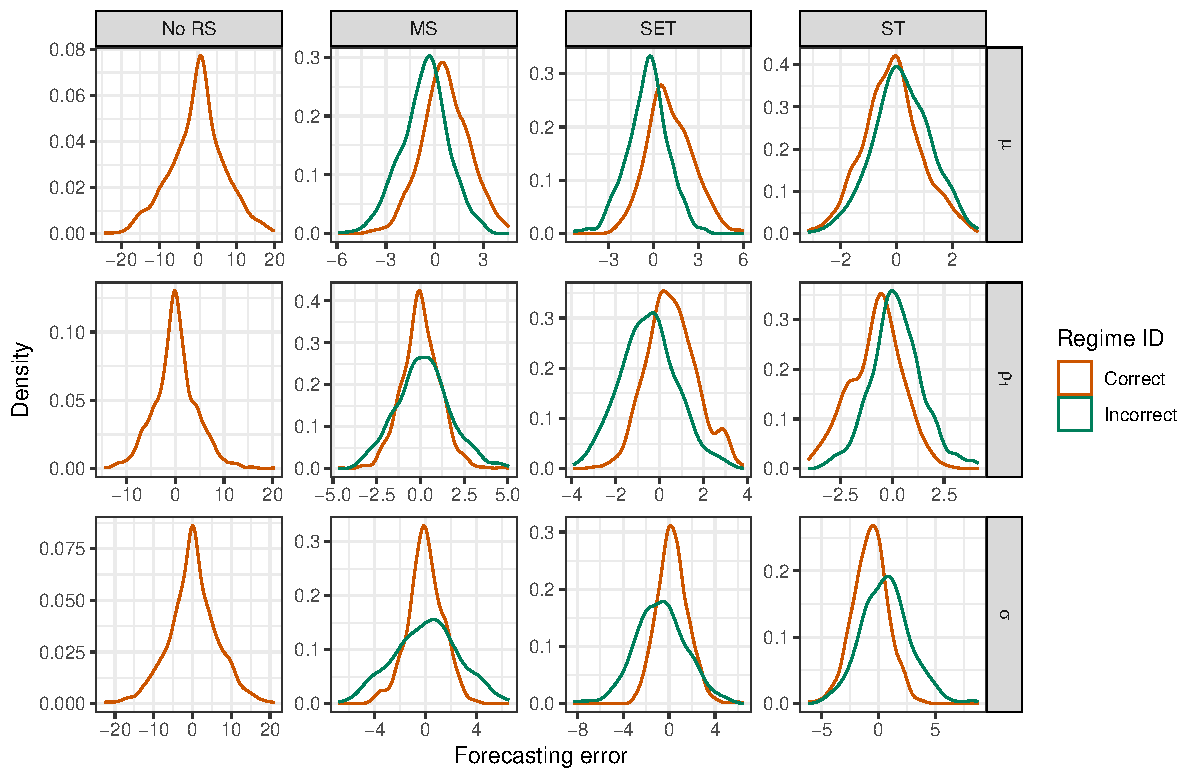
\includegraphics[width=\linewidth,height=0.4\textheight,keepaspectratio]{../../outputs/exploratory/rmse_regimes_r1_nors.pdf}

}

\end{figure}%

\begin{figure}

\caption{\label{fig-rp-ms}Regime and series prediction - MS}

\centering{

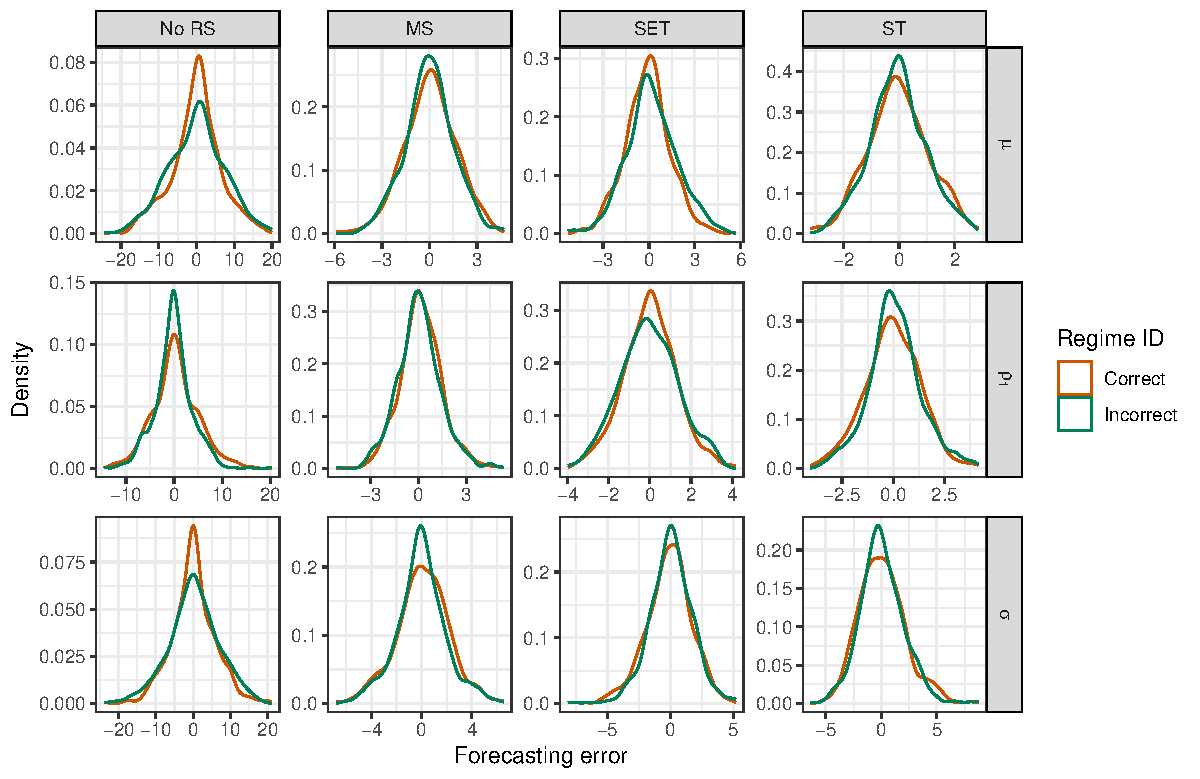
\includegraphics[width=\linewidth,height=0.4\textheight,keepaspectratio]{../../outputs/exploratory/rmse_regimes_r2_ms.pdf}

}

\end{figure}%

\begin{figure}

\caption{\label{fig-rp-set}Regime and series prediction - SET}

\centering{

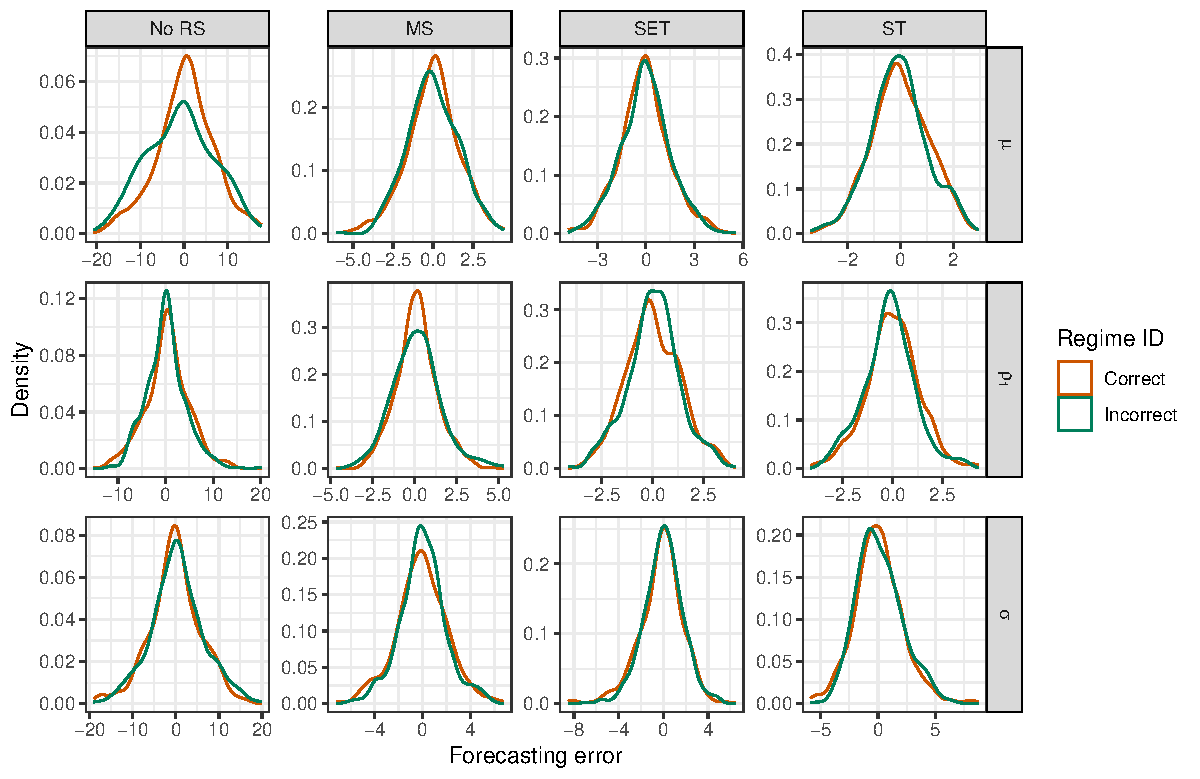
\includegraphics[width=\linewidth,height=0.4\textheight,keepaspectratio]{../../outputs/exploratory/rmse_regimes_r2_set_x.pdf}

}

\end{figure}%

\begin{figure}

\caption{\label{fig-rp-st}Regime and series prediction - ST}

\centering{

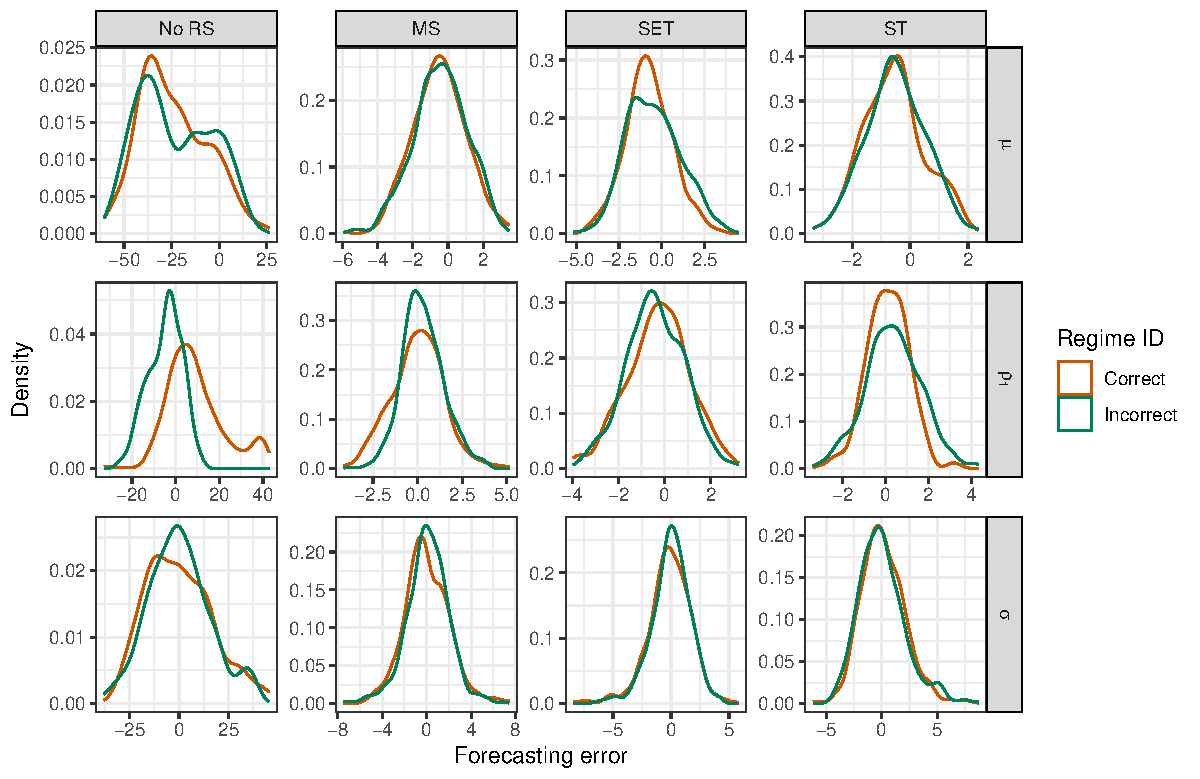
\includegraphics[width=\linewidth,height=0.4\textheight,keepaspectratio]{../../outputs/exploratory/rmse_regimes_r2_st.pdf}

}

\end{figure}%

\begin{figure}

\caption{\label{fig-rp-km}Regime and series prediction - KM}

\centering{

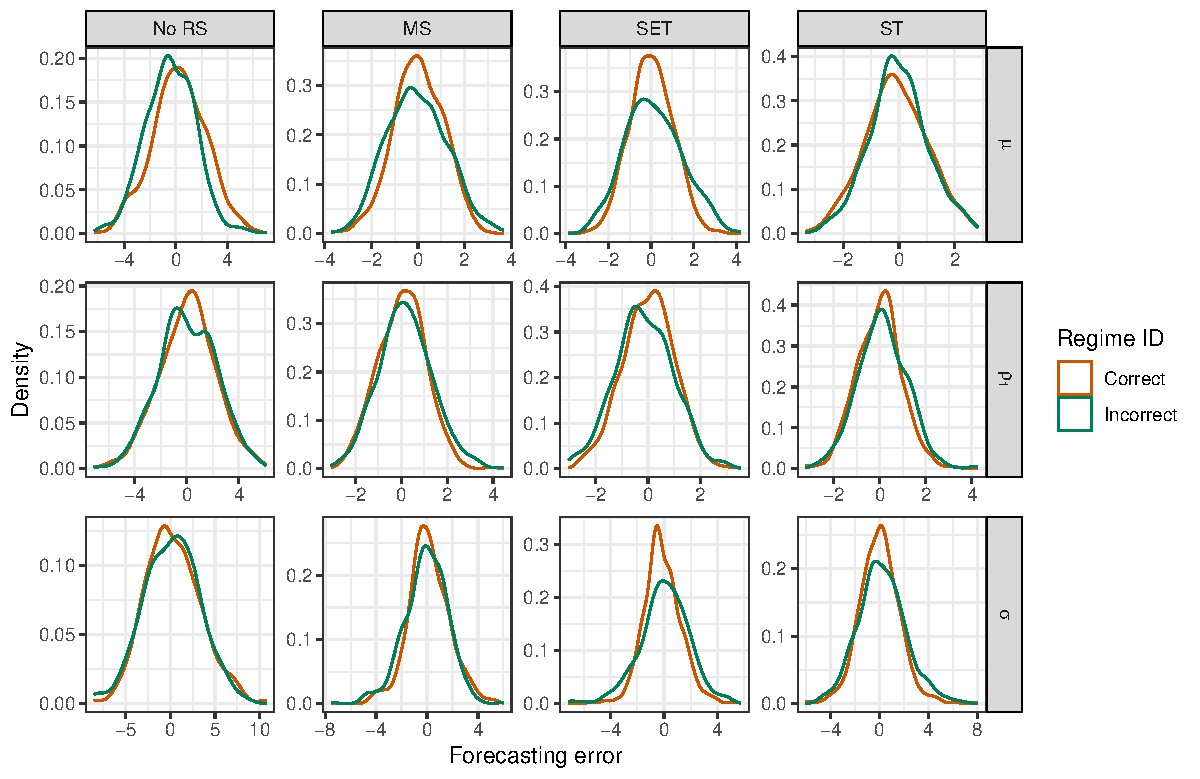
\includegraphics[width=\linewidth,height=0.4\textheight,keepaspectratio]{../../outputs/exploratory/rmse_regimes_r2_km.pdf}

}

\end{figure}%

\section{Performance analysis}\label{sec-perf}

In this section, the goal is to systematically analyze the performance
of models and how the regimes' distributions might affect and inform
performance. First, I examine the overall performance of each model
through their fixed effects. I (i) add controls to identify which
component of the models is most related to their performance; and (ii)
stratify the DGPs to understand how performance varies across scenarios.

I analyzing the models' interaction with the DGPs. I (i) evaluate the
effect of model-RGP mismatch and interact it with the DGP options to
determine if the mismatch effect varies across scenarios; (ii) analyze
specific model-DGP pairs; and (iii) consider an alternative way to
describe the DGPs, in terms of the RC metrics they generate, and assess
how each model performs against each profile of series. I consider
whether any results suggest practical recommendations for the
econometrician.

Then, I analyze which model component (estimated fit, \(r\), parameters,
or metrics) is most associated with each model's performance. For each
model, there are different points of interest for the econometrician.

Finally, regarding mis-specification, I test the hypothesis that
underestimating the number of regimes is less harmful when the regimes'
distributions are less separated, and whether the opposite is true for
overestimation.

All regressions use RMSE as the dependent variable, so higher
coefficient values imply worse performance associated with the given
variable. The metrics and parameters are normalized as
\(|x - \text{median}(x)| / \text{mad}(x)\), except for the RMSE. Some
metrics are not available for all observations, such as the ACF, which
requires at least one length-2 instance of each regime in the series.
Thus, the number of observations in each regression can vary. A
\(\Delta\) symbol represents the absolute difference between the
estimated value (often with \(y_{1:(T - H)}, \hat{r}_{1:(T - H)}\)) and
the analytical true value.

The results are conditional on the population of DGPs considered and
should not be interpreted as universal truths for any series.

\subsection{Models' fixed effects}\label{sec-perf-fe}

The fixed effects are presented in Table~\ref{tbl-fe_base}. This
excludes the no-RS and RF models. The first column, without controls,
indicates that SET and ST perform similarly and better than MS. This may
be due to the higher prevalence of threshold-based DGPs compared to
Markov-based ones in the DGP pool. All of them perform significantly
worse than KM.

To understand how the qualities of the models contribute to these fixed
effects, I add controls for matching the true vs.~estimated fit,
\(r\),\footnote{Controls include the binarized mean error, the
  \(\Delta\) average switches, and the \(\Delta\) average duration.}
parameters, and metrics' dispersion, then remove them one by one. A
better FE without a control means that the relationship between the
model and that control is a positive component in its FE. Comparing (2)
and (3), MS shows the highest improvement, given its flexible structure
that can fit very general data, compared to the rigidity of the
threshold-based models.

With Columns (2) and (4), we observe the counterpart effect: MS
struggles to match the regimes, given its geometric distribution that is
often not aligned with threshold-based regimes. ST performs slightly
worse than SET, but this is because the regimes measure is binarized and
does not utilize the continuity of ST regimes. The only model with a
positive relationship is KM, which assumes no specific hypothesis on the
regime structure. This particular relationship between KM and regime
matching will help explain further results.

Comparing (2) and (5), none of the models' performance improves by
matching the parameters, especially ST, which can often generate very
unreasonable estimates, as noted in Appendix~\ref{sec-app-diag-params}.
In contrast, matching the metrics explains a large part of the models'
fixed effects, especially for ST, but not for KM. This is an important
realization, as the effects of parameters and metrics might initially
seem interchangeable, but they are not.

\begin{table}[!htbp]

\caption{\label{tbl-fe_base}Models' fixed effects - baseline and
controls}

\centering{

\begin{tabular}{@{\extracolsep{5pt}}lcccccc} 
\\[-1.8ex]\hline 
\hline \\[-1.8ex] 
\\[-1.8ex] & \multicolumn{6}{c}{RMSE} \\ 
\\[-1.8ex] & (1) & (2) & (3) & (4) & (5) & (6)\\ 
\hline \\[-1.8ex] 
 MS & 1.799$^{***}$ & 1.249$^{***}$ & 1.225$^{***}$ & 1.413$^{***}$ & 1.275$^{***}$ & 1.270$^{***}$ \\ 
  & (0.011) & (0.006) & (0.006) & (0.009) & (0.006) & (0.005) \\ 
  SET & 1.698$^{***}$ & 1.290$^{***}$ & 1.300$^{***}$ & 1.232$^{***}$ & 1.342$^{***}$ & 1.231$^{***}$ \\ 
  & (0.011) & (0.005) & (0.005) & (0.008) & (0.005) & (0.005) \\ 
  ST & 1.672$^{***}$ & 1.234$^{***}$ & 1.241$^{***}$ & 1.294$^{***}$ & 1.300$^{***}$ & 1.179$^{***}$ \\ 
  & (0.011) & (0.006) & (0.006) & (0.010) & (0.005) & (0.005) \\ 
$R^2$ &  & yes &  & yes & yes & yes \\
  regimes &  & yes & yes &  & yes & yes \\
$\Delta$ params. &  & yes & yes & yes &  & yes \\
$\Delta$ metrics &  & yes & yes & yes & yes &  \\
 \hline \\[-1.8ex] 
Observations & 59,225 & 44,009 & 44,009 & 48,580 & 44,010 & 53,156 \\ 
R$^{2}$ & 0.563 & 0.872 & 0.869 & 0.787 & 0.867 & 0.854 \\ 
Adjusted R$^{2}$ & 0.563 & 0.872 & 0.869 & 0.787 & 0.867 & 0.854 \\ 
Residual Std. Error & 1.519 & 0.518 & 0.524 & 1.015 & 0.529 & 0.568 \\ 
\hline 
\hline \\[-1.8ex] 
\textit{Note:}  & \multicolumn{6}{r}{$^{*}$p$<$0.1; $^{**}$p$<$0.05; $^{***}$p$<$0.01} \\ 
\end{tabular} 


}

\end{table}%

To understand how these fixed effects vary across different DGPs,
Table~\ref{tbl-fe_strat} shows the fixed effects with no controls but
with stratifications in the dataset. It excludes the no-RS model. Column
(1) is the same as before but now includes the RF model, which is second
to KM, partially due to its `generic' overfitted hyperparameterization.
While the MS model showed a poorer relationship with regime matching, in
column (2), we see that its flexibility pays off, as it performs better
in asymmetric regimes. The RF model shows similar behavior. In Column
(3), ST deals better with small regime natures than SET. This is related
to Table~\ref{tbl-metrics_sep_t}, where SET series were not fully
separated in small regime natures, while in the ST ones they were, and
this is reflected in the fixed effects.

Changes in \(\mu\) (4) generate a better setup for separating the series
via threshold, improving SET and ST. Changes in \(\rho\) (5) are poorly
captured by ST but nicely captured by MS and KM. In a \(\sigma\) change
(6), everyone performs worse, as it is overall harder to forecast. The
overfitting of RF is evident here, as it presents the highest change
from column (1), while ST shows one of the best robustness, in line with
its ability to handle explosive volatility, as noted by Verne (2021).

The KM model's FE changes the least across stratifications, on average
0.17, followed by ST, with \(0.23\). These are characteristics of more
general models that have some `flavor' of universal approximation power.
The ability of ST to deal with some of the harder DGPs is related to its
relationship to the complexity of a Neural Network, as discussed by
Medeiros (2000), granted that the present setup with \(S = 2\) does not
reach its full potential. The RF model is also kept shy of its
potential, and while it would be interesting to have a
better-architected RF, this benchmark already shows its improvement over
the traditional models while making it clear that overfit is a risk.

\begin{table}[!htbp]

\caption{\label{tbl-fe_strat}Models fixed effects - across
stratifications}

\centering{

\begin{tabular}{@{\extracolsep{5pt}}lcccccc} 
\\[-1.8ex]\hline 
\hline \\[-1.8ex] 
\\[-1.8ex] & \multicolumn{6}{c}{RMSE} \\ 
\\[-1.8ex] & (1) & (2) & (3) & (4) & (5) & (6)\\ 
\hline \\[-1.8ex] 
 MS & 1.781$^{***}$ & 1.308$^{***}$ & 1.676$^{***}$ & 1.782$^{***}$ & 1.569$^{***}$ & 1.987$^{***}$ \\ 
  & (0.009) & (0.005) & (0.013) & (0.015) & (0.015) & (0.017) \\ 
  SET & 1.687$^{***}$ & 1.322$^{***}$ & 1.607$^{***}$ & 1.601$^{***}$ & 1.529$^{***}$ & 1.932$^{***}$ \\ 
  & (0.009) & (0.005) & (0.013) & (0.015) & (0.015) & (0.017) \\ 
  ST & 1.632$^{***}$ & 1.313$^{***}$ & 1.553$^{***}$ & 1.391$^{***}$ & 1.611$^{***}$ & 1.884$^{***}$ \\ 
  & (0.009) & (0.005) & (0.013) & (0.016) & (0.015) & (0.018) \\ 
  KM & 1.308$^{***}$ & 1.132$^{***}$ & 1.254$^{***}$ & 1.182$^{***}$ & 1.180$^{***}$ & 1.562$^{***}$ \\ 
  & (0.009) & (0.005) & (0.013) & (0.015) & (0.015) & (0.017) \\ 
  RF & 1.588$^{***}$ & 1.214$^{***}$ & 1.578$^{***}$ & 1.320$^{***}$ & 1.508$^{***}$ & 1.910$^{***}$ \\ 
  & (0.009) & (0.005) & (0.013) & (0.016) & (0.015) & (0.017) \\ 
  Strat. & none & asym. RGP & small RN & $\mu$ RN & $\rho_1$ RN & $\sigma$ RN \\
 \hline \\[-1.8ex] 
Observations & 99,944 & 44,491 & 50,172 & 32,357 & 33,925 & 33,662 \\ 
R$^{2}$ & 0.603 & 0.879 & 0.591 & 0.589 & 0.595 & 0.639 \\ 
Adjusted R$^{2}$ & 0.603 & 0.879 & 0.591 & 0.589 & 0.595 & 0.639 \\ 
Residual Std. Error & 1.302 & 0.467 & 1.280 & 1.229 & 1.224 & 1.398 \\ 
\hline 
\hline \\[-1.8ex] 
\textit{Note:}  & \multicolumn{6}{r}{$^{*}$p$<$0.1; $^{**}$p$<$0.05; $^{***}$p$<$0.01} \\ 
\end{tabular} 


}

\end{table}%

\subsection{Model and DGP interaction}\label{sec-perf-mis}

\subsubsection{Mis-specification of RGP
family}\label{mis-specification-of-rgp-family}

To study the effect of mis-specification, Table~\ref{tbl-mis_is} defines
mis-specification as ``the family of the model being different than the
family of the RGP''. Only the MS, SET, and ST models are included. The
baseline effect of mis-specification is an RMSE increase of \(0.52\). To
further understand how this effect changes across stratifications,
consider columns (2-6). (2): MS models suffer more, in line with
previous results, while ST models suffer less. (3): Mis-estimating an RS
model in a non-RS RGP is disastrous, and in light of that,
mis-specification across RS RGPs is not as relevant. This will be
further explored in the next subsection.

In (4), asymmetric regimes are harder to estimate, so sometimes
mis-specification helps. (5): Similar to before, \(\sigma\) changes make
forecasting harder, and this effect is compounded by mis-specification;
for the other two parameters, the effect is similar. Finally, (6) shows
that in small RNs, estimating the wrong regime generates a smaller
error, so mis-specifying the RGP is not too problematic.

\begin{table}[!htbp]

\caption{\label{tbl-mis_is}Models and DGPs mis-specification}

\centering{


% Table created by stargazer v.5.2.3 by Marek Hlavac, Social Policy Institute. E-mail: marek.hlavac at gmail.com
% Date and time: ter, mai 05, 2026 - 21:08:28
\begin{table}[!htbp] \centering 
  \caption{} 
  \label{} 
\begin{tabular}{@{\extracolsep{5pt}}lc} 
\\[-1.8ex]\hline 
\hline \\[-1.8ex] 
 & \multicolumn{1}{c}{\textit{Dependent variable:}} \\ 
\cline{2-2} 
\\[-1.8ex] & rmse \\ 
\hline \\[-1.8ex] 
 is\_mis & 0.010 (0.013) \\ 
  Constant & 1.376$^{***}$ (0.011) \\ 
 \hline \\[-1.8ex] 
Observations & 11,804 \\ 
R$^{2}$ & 0.0001 \\ 
Adjusted R$^{2}$ & $-$0.00003 \\ 
Residual Std. Error & 0.585 \\ 
F Statistic p-value & 0.422 \\ 
\hline 
\hline \\[-1.8ex] 
\textit{Note:}  & \multicolumn{1}{r}{$^{*}$p$<$0.1; $^{**}$p$<$0.05; $^{***}$p$<$0.01} \\ 
\end{tabular} 
\end{table} 


}

\end{table}%

\subsubsection{Specific model-RGP
mis-specifications}\label{sec-perf-mis-pairs}

Misspecification in general is detrimental. However, stratifying by each
of the RGP families in Table~\ref{tbl-mis_rgp} shows that each model
(line) has similar values across the different RGPs (columns). This
confirms that correctly specifying the RGP family is not the most
critical factor for performance.

With SET, the values are positive, meaning that the model performs
slightly better with no-RS series. For ST, the values are highly
negative, meaning that no-RS series generate disastrous results, and
this is reflected in Table~\ref{tbl-mis_is} column (3). Conversely, KM
performs exceptionally well when there is no regime switching. For MS,
RS or no-RS matters less. The invariance to RGP, especially between SET
and ST, is intriguing and, in some ways, contradicts the results of
Aydın; Mermi (2022), although a broader diversity of SET and ST models
would be required for a proper comparison.

\begin{table}[!htbp]

\caption{\label{tbl-mis_rgp}Models and RGP pairs mis-specification}

\centering{

\begin{tabular}{@{\extracolsep{\fill}}l|rrr}
\toprule\toprule
 & \multicolumn{3}{c}{{RGP}} \\ 
\cmidrule(lr){2-4}
Model & MS & SET & ST \\ 
\midrule\addlinespace[2.5pt]
MS & 0.001 (0.029) & 0.005 (0.029) & 0.007 (0.029) \\ 
SET & 0.066** (0.03) & 0.065** (0.03) & 0.066** (0.03) \\ 
ST & -1.657*** (0.035) & -1.644*** (0.035) & -1.633*** (0.035) \\ 
KM & 2.113*** (0.028) & 2.05*** (0.028) & 2.142*** (0.028) \\ 
\midrule\addlinespace[2.5pt]
\multicolumn{2}{l|}{Observations} & \multicolumn{2}{l}{100840} \\
\multicolumn{2}{l|}{$R^2$,$~$ Adjusted $R^2$} & \multicolumn{2}{l}{0.826,$~~~$0.826} \\
\multicolumn{2}{l|}{Resid. SE,$~$ F stat. p-value} & \multicolumn{2}{l}{0.884,$~~~$<0.001} \\
\bottomrule\bottomrule
\end{tabular}
\begin{minipage}{\linewidth}\centering
\vspace{.05em}
\emph{Note:}  \(^{*}\)p\textless{}0.1; \(^{**}\)p\textless{}0.05; \(^{***}\)p\textless{}0.01\\
\end{minipage}


}

\end{table}%

RGP alone does not explain the mis-specification effect, but the
interaction with RN was deemed relevant in the exploratory analysis.
Table~\ref{tbl-mis_rgp_full} shows the coefficients for the interactions
between model, RGP, and RN,\footnote{Controls include model, parameter
  change, and RGP family FEs, plus interactions between the last two.}
but we still observe a similar result of `invariance' within each
`panel' (RGP-model pair) of the table, except for KM.

\begin{table}[!htbp]

\caption{\label{tbl-mis_rgp_full}Models, RGPs, and RNs
mis-specification}

\centering{

\begin{tabular}{@{\extracolsep{\fill}}l|l|lllr}
\toprule\toprule
\multicolumn{2}{l}{} & \multicolumn{4}{c}{{Model}} \\ 
\cmidrule(lr){3-6}
RGP & SGP & MS & SET & ST & KM \\ 
\midrule\addlinespace[2.5pt]
No RS & \(\mu\) & 0.02 (0.048) & -0.055 (0.052) & 2.085*** (0.091) & -2.868*** (0.047) \\ 
 & \(\rho_{1}\) & -0.015 (0.047) & -0.034 (0.048) & 1.927*** (0.052) & -1.522*** (0.047) \\ 
 & \(\sigma\) & -0.031 (0.048) & 0.048 (0.05) & 1.825*** (0.056) &  \\ 
 &  &  &  &  &  \\ 
MS & \(\mu\) & -0.012 (0.038) & -0.008 (0.038) & 0.012 (0.038) & -0.028 (0.038) \\ 
 & \(\rho_{1}\) & -0.011 (0.038) & -0.004 (0.038) & -0.007 (0.038) & 0.073* (0.038) \\ 
 & \(\sigma\) & -0.003 (0.038) & -0.001 (0.038) & -0.004 (0.038) &  \\ 
 &  &  &  &  &  \\ 
SET & \(\mu\) & 0.001 (0.038) & -0.01 (0.038) & 0.043 (0.038) & -0.16*** (0.038) \\ 
 & \(\rho_{1}\) & -0.011 (0.038) & -0.011 (0.038) & 0.008 (0.038) & 0.003 (0.038) \\ 
 & \(\sigma\) & -0.003 (0.038) & 0.006 (0.038) & -0.017 (0.038) &  \\ 
 &  &  &  &  &  \\ 
ST & \(\mu\) & -0.01 (0.038) & 0 (0.038) & 0.082** (0.038) & 0.175*** (0.038) \\ 
 & \(\rho_{1}\) & -0.006 (0.038) & -0.013 (0.038) & -0.013 (0.038) & -0.021 (0.038) \\
\midrule\addlinespace[2.5pt]
\multicolumn{3}{l|}{Observations} & \multicolumn{1}{l}{100840} \\
\multicolumn{3}{l|}{$R^2$,$~$ Adjusted $R^2$} & \multicolumn{1}{l}{0.84,$~~~$0.84} \\
\multicolumn{3}{l|}{Resid. SE,$~$ F stat. p-value} & \multicolumn{1}{l}{0.848,$~~~$<0.001} \\
\bottomrule\bottomrule
\end{tabular}
\begin{minipage}{\linewidth}\centering
\vspace{.05em}
\emph{Note:}  \(^{*}\)p\textless{}0.1; \(^{**}\)p\textless{}0.05; \(^{***}\)p\textless{}0.01\\
\end{minipage}


}

\end{table}%

\subsubsection{Models and RC metrics}\label{models-and-rc-metrics}

Fortunately, the point of this work is that the RC metrics provide
another way to characterize the DGP, and in some ways, a more general
one than the RGP family `label'. I construct similar tables interacting
each model with the profiles of (dispersion of) metrics in the series.
As the whole profile of metrics is important, all of the interactions of
\(\mod \cdot d(\mu(.)) \cdot d(\rho_1(.)) \cdot d(\sigma(.))\) are
included as controls.

Table~\ref{tbl-mis_metrics_sim} uses the true values of the metrics.
After controlling for the interactions, SET, ST, and KM have a negative
effect when estimated on series with high average separation, given the
easier time separating series via thresholds. For MS, we do not observe
significant effects, and not much can be said about it without deeper
analysis. ST seems to struggle with high separation in ACF. KM benefits
from SD differentiation.

\begin{table}[!htbp]

\caption{\label{tbl-mis_metrics_sim}Models and true RC metrics}

\centering{

\begin{table}[t]
\fontsize{12.0pt}{14.0pt}\selectfont
\begin{tabular*}{\linewidth}{@{\extracolsep{\fill}}l|rrr}
\toprule
RGP \(\diagdown\) Model & SET & ST & MS \\ 
\midrule\addlinespace[2.5pt]
SET & -0.054 (0.09) & -0.001 (0.068) & -0.009 (0.084) \\ 
ST & 1.482 (0.09)*** & -0.052 (0.068) & 0.157 (0.084)* \\ 
MS & 0.002 (0.091) & 0 (0.068) & -0.013 (0.084) \\ 
\bottomrule
\end{tabular*}
\begin{minipage}{\linewidth}
\vspace{.05em}
\emph{Note:}  \(^{*}\)p\$\textless{}\$0.1; \(^{**}\)p\$\textless{}\$0.05; \(^{***}\)p\$\textless{}\$0.01\\
\end{minipage}
\end{table}



}

\end{table}%

It is important to check if the estimated metrics generate similar
results, as they are observable by the econometrician. This is done in
Table~\ref{tbl-mis_metrics_est}. Unfortunately, the results vary widely.
As noted in Figure~\ref{fig-metrics_diff}, the models do not perfectly
match the metrics, which blurs the relationship found in the previous
table.

\begin{table}[!htbp]

\caption{\label{tbl-mis_metrics_est}Models and estimated RC metrics}

\centering{

\begin{tabular}{@{\extracolsep{\fill}}l|rrr}
\toprule
 & \multicolumn{3}{c}{{Metric}} \\ 
\cmidrule(lr){2-4}
Model & Avg & ACF & SD \\ 
\midrule\addlinespace[2.5pt]
SET & -0.391*** (0.037) & -0.009 (0.022) & -0.094 (0.227) \\ 
ST & -0.129*** (0.006) & 0.183*** (0.023) & -0.607*** (0.234) \\ 
MS & -0.529 (0.325) & 0.338*** (0.026) & 0.821*** (0.236) \\ 
\bottomrule
\end{tabular}
\begin{minipage}{\linewidth}\centering
\vspace{.05em}
\emph{Note:}  \(^{*}\)p\textless{}0.1; \(^{**}\)p\textless{}0.05; \(^{***}\)p\textless{}0.01\\
\end{minipage}


}

\end{table}%

Also recall, the metric estimation error varied across the unobservable
RN, which means that these general relationships might not be too
informative. Table~\ref{tbl-mis_metrics_est_strat} shows the values of
interactions between models, metrics, and which parameter
changes.\footnote{Controls include model, metric FEs, and interactions:
  metric\(^2\) (with itself) and model \(\cdot\) metric\(^2\).} The
omitted group is the interaction with \(\mu\). For example, a big ACF
difference is only a bad indicator when the parameter changing was
\(\sigma\), not \(\rho_1\) (for SET and KM); average separation is often
bad when \(\mu\) is fixed.

\begin{table}[!htbp]

\caption{\label{tbl-mis_metrics_est_strat}Models and estimated RC
metrics - RN interactions}

\centering{

\begin{tabular}{@{\extracolsep{\fill}}l|l|rrrr}
\toprule\toprule
\multicolumn{2}{l}{} & \multicolumn{4}{c}{{Model}} \\ 
\cmidrule(lr){3-6}
Metric & SGP & MS & SET & ST & KM \\ 
\midrule\addlinespace[2.5pt]
\(d(\hat{\mu}(.))\) & \(\rho_{1}\) & 0.025* (0.013) & -0.039*** (0.012) & 0.107*** (0.023) & 0.011 (0.009) \\ 
 & \(\sigma\) & 0.053*** (0.011) & 0.025** (0.012) & 0.113*** (0.023) & 0.05*** (0.009) \\ 
 &  &  &  &  &  \\ 
\(d(\hat{\rho}_1(.))\) & \(\rho_{1}\) & -0.005 (0.008) & -0.01 (0.006) & -0.014* (0.007) & 0.004 (0.015) \\ 
 & \(\sigma\) & 0.004 (0.008) & 0.05*** (0.006) & 0.013 (0.008) & 0.119*** (0.016) \\ 
 &  &  &  &  &  \\ 
\(d(\hat{\sigma}(.))\) & \(\rho_{1}\) & -0.036*** (0.006) & 0.053*** (0.011) & 0.007 (0.015) & -0.006 (0.014) \\ 
 & \(\sigma\) & -0.017*** (0.006) & 0.061*** (0.01) & 0.012 (0.014) & 0.015 (0.013) \\ 
\midrule\addlinespace[2.5pt]
\multicolumn{3}{l|}{Observations} & \multicolumn{1}{l}{88126} \\
\multicolumn{3}{l|}{$R^2$,$~$ Adjusted $R^2$} & \multicolumn{1}{l}{0.737,$~~~$0.737} \\
\multicolumn{3}{l|}{Resid. SE,$~$ F stat. p-value} & \multicolumn{1}{l}{1.012,$~~~$<0.001} \\
\bottomrule\bottomrule
\end{tabular}
\begin{minipage}{\linewidth}\centering
\vspace{.05em}
\emph{Note:}  \(^{*}\)p\textless{}0.1; \(^{**}\)p\textless{}0.05; \(^{***}\)p\textless{}0.01\\
\end{minipage}


}

\end{table}%

The results of this section could be used as a practical recommendation
to the econometrician, e.g., ``if your KM-based estimated regimes have
high volatility separation, the model selection is sound, as the others
often struggle with such series''. However, this is currently very
limited because: (i) the metrics' estimation error hides the true
relationships between model and metrics; (ii) as noted in
Section~\ref{sec-sep-in}, the three metrics used are not enough to fully
characterize each DGP, thus the results vary widely across the
unobservable RN; (iii) while the use of RC metrics abstracts away from
specific DGPs, the results are still conditional on the limited
population used in this work.

Some strategies could be employed to improve the estimated metrics'
meaning, such as using weights proportional to how close each data point
is to a regime change, considering other dispersion measures, or even
silhouette-like scores instead of simple absolute differences. On the
front of characterizing the DGPs, more metrics should be added, such as
3rd and 4th moments, more ACF lags, and more general distribution
distance measures. Perhaps regime-unconditional and residual metrics --
merging the usual model diagnostics in this analysis -- could also
improve the characterization. Overall, the present exercise, while not
perfect, is a step towards a more general and informative way to
characterize the DGPs and hopefully generate practical results for the
econometrician.

\subsection{Identification and performance}\label{sec-perf-id}

In the Models' Fixed Effect section, we discussed the qualities of the
models. It can be interesting to analyze separately how matching each of
the characteristics of the DGPs relates to the RMSE of an estimation.
This is done in Table~\ref{tbl-match}. Recall the definition of
\(\Delta\) provided at the beginning of this section: a positive
coefficient means that a higher difference between the true and
estimated values is associated with a higher RMSE.

There are counterintuitive relationships between \(R^2\),
\(BME(r)\),\footnote{Binarized mean error, the proportion of
  observations where the estimated regime is different from the true
  one.} and RMSE: better fit, more error. These will be better analyzed
below. The second column shows that \(\rho_1\) can have an adverse
effect, as it did in fact have the least straightforward relationship
with RGP, RN, and model interactions. A similar result is seen in the
matching of metrics.

\begin{table}[!htbp]

\caption{\label{tbl-match}RMSE and identification}

\centering{


=================================================================================================================================================================
                                                                                 Dependent variable:                                                             
                    ---------------------------------------------------------------------------------------------------------------------------------------------
                                                                                        rmse                                                                     
                               (1)                       (2)                          (3)                          (4)                           (5)             
-----------------------------------------------------------------------------------------------------------------------------------------------------------------
regimes_bme             -0.064*** (0.015)                                                                                                                        
switches_diff                                     -0.286*** (0.007)                                                                                              
duration_diff                                      0.097*** (0.006)                                                                                              
r2                                                                             1.962*** (0.014)                                                                  
mu_diff                                                                                                      1.637*** (0.015)                                    
rho1_diff                                                                                                    0.107*** (0.014)                                    
sigma_diff                                                                                                   0.166*** (0.014)                                    
avg_diff                                                                                                                                  1.928*** (0.021)       
acf_diff                                                                                                                                    0.017 (0.014)        
sd_diff                                                                                                                                   0.731*** (0.022)       
-----------------------------------------------------------------------------------------------------------------------------------------------------------------
Observations                 82,455                     52,988                      82,455                        82,455                       72,721            
R2                           0.0002                     0.030                        0.198                        0.145                         0.335            
Adjusted R2                  0.0002                     0.030                        0.198                        0.145                         0.335            
Residual Std. Error    4.415 (df = 82454)         1.423 (df = 52986)          3.955 (df = 82454)            4.083 (df = 82452)           3.765 (df = 72718)      
NA p-value & 0NA
=================================================================================================================================================================
Note:                                                                                                                                 *p<0.1; **p<0.05; ***p<0.01


}

\end{table}%

To properly analyze the first column, Table~\ref{tbl-match_r2}
stratifies the fit and regime effects by model. We observe that regime
errors only have a negative relationship with no-RS and KM, two models
that have some `disregard' for the regime structure, while for the
traditional models, smaller errors improve performance. This aligns with
Dacco; Satchell (1999), who found that minor errors in the regime
variable can lead to large forecasting errors. Apparently, KM is an
exception to that rule, given the lack of parametric assumptions on the
RGP. For the fit, the positive relationship still stands, meaning that
fitting the regime is not a good guide for performance. The RF has the
highest \(R^2\) coefficient, another indication of its overfitting. MS
has one similar to no-RS, attesting to its flexibility, but not as small
as KM.

\begin{table}[!htbp]

\caption{\label{tbl-match_r2}RMSE and \(R^2\) across models}

\centering{

\begin{tabular}{@{\extracolsep{5pt}}lcc} 
\\[-1.8ex]\hline 
\hline \\[-1.8ex] 
\\[-1.8ex] & \multicolumn{2}{c}{RMSE} \\ 
\\[-1.8ex] & $x = R^2$ & $x = BME(r)$\\ 
\hline \\[-1.8ex] 
  $x ~ \cdot$ No RS & 0.749$^{***}$ (0.009) & $-$0.914$^{***}$ (0.012) \\ 
  $x ~ \cdot$ MS & 0.746$^{***}$ (0.009) &    0.497$^{***}$ (0.021)     \\ 
  $x ~ \cdot$ SET & 0.851$^{***}$ (0.010) &   0.329$^{***}$ (0.018)     \\ 
  $x ~ \cdot$ ST & 0.849$^{***}$ (0.013) &    0.347$^{***}$ (0.012)     \\ 
  $x ~ \cdot$ KM & 0.467$^{***}$ (0.009) &    $-$0.310$^{***}$ (0.016)  \\ 
  $x ~ \cdot$ RF & 1.482$^{***}$ (0.011) &      \\ 
 \hline \\[-1.8ex] 
Observations & 120,850 & 100,840 \\ 
R$^{2}$ & 0.288 & 0.072 \\ 
Residual Std. Error & 1.786 & 2.039 \\ 
F Statistic p-value & <0.001 & <0.001 \\ 
\hline 
\hline \\[-1.8ex] 
\textit{Note:}  & \multicolumn{2}{r}{$^{*}$p$<$0.1; $^{**}$p$<$0.05; $^{***}$p$<$0.01} \\ 
\end{tabular} 


}

\end{table}%

To further analyze the effect of matching the metrics,
Table~\ref{tbl-match_metrics} shows model-metric interactions. MS has a
massive improvement when matching the average and decent results on
volatility. SET is similar but overall matching matters less. For ST,
matching the average matters less, but it is more important for ACF and
volatility. KM is overall the most balanced, with a decent relationship
with all metrics.

\begin{table}[!htbp]

\caption{\label{tbl-match_metrics}RMSE and metrics identification across
models}

\centering{

\begin{tabular}{@{\extracolsep{\fill}}l|rrr}
\toprule
 & \multicolumn{3}{c}{{RGP}} \\ 
\cmidrule(lr){2-4}
Model & SET & ST & MS \\ 
\midrule\addlinespace[2.5pt]
SET & 1.107*** (0.01) & 0.332*** (0.006) & 1.955*** (0.041) \\ 
ST & 0.234*** (0.004) & 0.976*** (0.041) & 1.884*** (0.042) \\ 
MS & 0.445*** (0.005) & 2.322*** (0.034) & 2.113*** (0.018) \\ 
\bottomrule
\end{tabular}
\begin{minipage}{\linewidth}\centering
\vspace{.05em}
\emph{Note:}  \(^{*}\)p\textless{}0.1; \(^{**}\)p\textless{}0.05; \(^{***}\)p\textless{}0.01\\
\end{minipage}


}

\end{table}%

Again, it might be important to check the interaction with RN. This is
done in Table~\ref{tbl-match_metrics_strat}. The same controls are used.
The effects are generally different when \(\mu\) changes, but not so
much across \(\rho_1\) or \(\sigma\). Additionally, the interactions are
overall smaller, indicating a smaller dependence on these non-observable
characteristics of the DGPs.

\begin{table}[!htbp]

\caption{\label{tbl-match_metrics_strat}Models and estimated RC metrics
- RN interactions}

\centering{

\begin{tabular}{@{\extracolsep{\fill}}l|l|rrrr}
\toprule\toprule
\multicolumn{2}{l}{} & \multicolumn{4}{c}{{Model}} \\ 
\cmidrule(lr){3-6}
Metric & SGP & MS & SET & ST & KM \\ 
\midrule\addlinespace[2.5pt]
\(d(\hat{\mu}(.))\) & \(\rho_{1}\) & -0.067*** (0.013) & 0.012 (0.011) & 0.127*** (0.021) & -0.004 (0.009) \\ 
 & \(\sigma\) & -0.008 (0.011) & 0.099*** (0.011) & 0.154*** (0.021) & 0.046*** (0.008) \\ 
 &  &  &  &  &  \\ 
\(d(\hat{\rho}_1(.))\) & \(\rho_{1}\) & -0.006 (0.014) & -0.025** (0.011) & -0.182*** (0.014) & -0.039 (0.026) \\ 
 & \(\sigma\) & 0.002 (0.013) & 0.076*** (0.011) & -0.093*** (0.015) & 0.073** (0.034) \\ 
 &  &  &  &  &  \\ 
\(d(\hat{\sigma}(.))\) & \(\rho_{1}\) & -0.048*** (0.01) & -0.04*** (0.015) & -0.074*** (0.025) & 0.007 (0.027) \\ 
 & \(\sigma\) & -0.028*** (0.009) & -0.074*** (0.015) & -0.143*** (0.025) & 0.028 (0.024) \\ 
\midrule\addlinespace[2.5pt]
\multicolumn{3}{l|}{Observations} & \multicolumn{1}{l}{89065} \\
\multicolumn{3}{l|}{$R^2$,$~$ Adjusted $R^2$} & \multicolumn{1}{l}{0.736,$~~~$0.736} \\
\multicolumn{3}{l|}{Resid. SE,$~$ F stat. p-value} & \multicolumn{1}{l}{1.051,$~~~$<0.001} \\
\bottomrule\bottomrule
\end{tabular}
\begin{minipage}{\linewidth}\centering
\vspace{.05em}
\emph{Note:}  \(^{*}\)p\textless{}0.1; \(^{**}\)p\textless{}0.05; \(^{***}\)p\textless{}0.01\\
\end{minipage}


}

\end{table}%

These results could also be taken as practical recommendations, e.g.,
``if the econometrician has a belief about the true volatility
dispersion, and the ST estimated doesn't match it, it might be a
problem''. A substitute for belief would be a more general measure of
variation of the metric across time, such as the SD of the rolling
metric.\footnote{The prediction power of this measure, for the true
  metric dispersion, must be studied.} This interpretation is less
useful since such beliefs are not common, and we have the same external
validity issues as before.

There are other matchable characteristics of the models, such as the
\(\tau\) for threshold models, the \(\gamma\) for ST, and transition
probabilities for MS. They are not included here, as they are not
directly comparable across models and do not generate interesting
analysis.

\subsection{Incorrect number of regimes}\label{sec-perf-nr}

This section analyzes how the models perform when the assumed number of
regimes \(\hat{S}\) is different from the true one \(S\). In this
analysis, underestimating the number of regimes means estimating a
simple \(AR(1)\) with one of the two-regime RGPs, while overestimating
means estimating some of the two-regime models with a series generator
from a simple AR(1). The results should be interpreted as such.

In Table~\ref{tbl-regimes}, the overall effect of underestimation even
shows an improvement.{[}\^{}km-nors{]} With overestimation, we observe a
positive result of \(0.7\).\footnote{Controls include metrics FEs, and
  interactions of the \(S\) comparison with models, plus metrics with
  models, RGP family, and RN parameter.} Column (2) shows that all of
the metrics' interactions are negative. This means that when we
overestimate, if the regimes were highly different in terms of the
metrics, we have an attenuation of the adverse effect of the
misspecification. That is, it is very useful to be able to match these
big differences, even if we need to use more regimes than might be
necessary.

When we consider the opposite scenario in (3), the interactions are
still negative. But again, this is carried by KM, as if we remove it
from the sample, we get positive results throughout all the metrics.
Column (4) shows that with underestimation, but similar regimes, we have
an attenuation of the misspecification effect.

\begin{table}[!htbp]

\caption{\label{tbl-regimes}Mis-specification of the number of regimes}

\centering{

\begin{tabular}{@{\extracolsep{5pt}}lccc} 
\\[-1.8ex]\hline 
\hline \\[-1.8ex] 
\\[-1.8ex] & \multicolumn{3}{c}{RMSE} \\ 
\\[-1.8ex] & (1) & (2) & (3)\\ 
\hline \\[-1.8ex] 
 $\hat{S} < S$ & $-$0.809$^{***}$ (0.017) &  & $-$0.494$^{***}$ (0.023) \\ 
  $\hat{S} > S$ & 0.714$^{***}$ (0.020) & 1.981$^{***}$ (0.028) &  \\ 
  $\hat{S} > S$ : $d(\hat{\mu}(.))$ &  & $-$1.927$^{***}$ (0.029) &  \\ 
  $\hat{S} > S$ : $d(\hat{\rho}_1(.))$ &  & $-$2.166$^{***}$ (0.096) &  \\ 
  $\hat{S} > S$ : $d(\hat{\sigma}(.))$ &  & $-$2.727$^{***}$ (0.050) &  \\ 
  $\hat{S} < S$ : $d(\hat{\mu}(.))$ &  &  & 0.301$^{***}$ (0.032) \\ 
  $\hat{S} < S$ : $d(\hat{\rho}_1(.))$ &  &  & 0.426$^{***}$ (0.111) \\ 
  $\hat{S} < S$ : $d(\hat{\sigma}(.))$ &  &  & 0.517$^{***}$ (0.054) \\ 
  Constant & 1.479$^{***}$ (0.013) & 1.183$^{***}$ (0.013) & 1.580$^{***}$ (0.017) \\ 
Strat. & none & none & no KM \\
 \hline \\[-1.8ex] 
Observations & 81,970 & 81,970 & 61,128 \\ 
R$^{2}$ & 0.498 & 0.519 & 0.537 \\ 
Residual Std. Error & 0.938 & 0.918 & 1.005 \\ 
F Statistic p-value & <0.001 & <0.001 & <0.001 \\ 
\hline 
\hline \\[-1.8ex] 
\textit{Note:}  & \multicolumn{3}{r}{$^{*}$p$<$0.1; $^{**}$p$<$0.05; $^{***}$p$<$0.01} \\ 
\end{tabular}


}

\end{table}%

To stratify the effects by model, consider
Table~\ref{tbl-regimes_models}. As noted before, the ST model performs
poorly with single-regime data, while KM actually benefits from it. MS
is a little more robust than SET. Given the specific definition of
overestimation, this result is not perfectly comparable with Janczura;
Weron (2010), who found a perceived big sensitivity of \(\hat{S}\) in
the MS model.

\begin{table}[!htbp]

\caption{\label{tbl-regimes_models}Mis-specification of the number of
regimes}

\centering{

\begin{tabular}{@{\extracolsep{5pt}}lc} 
\\[-1.8ex]\hline 
\hline \\[-1.8ex] 
\\[-1.8ex] & RMSE \\ 
\hline \\[-1.8ex] 
  $\hat{S} > S$ : MS & 1.152$^{***}$ (0.022) \\ 
  $\hat{S} > S$ : SET & 1.177$^{***}$ (0.024) \\ 
  $\hat{S} > S$ : ST & 3.072$^{***}$ (0.031) \\ 
  $\hat{S} < S$ : KM & $-$0.964$^{***}$ (0.022) \\ 
  Constant & 1.297$^{***}$ (0.011) \\ 
 \hline \\[-1.8ex] 
Observations & 100,840 \\ 
R$^{2}$ & 0.564 \\ 
Adjusted R$^{2}$ & 0.564 \\ 
Residual Std. Error & 0.888 \\ 
F Statistic p-value & <0.001 \\ 
\hline 
\hline \\[-1.8ex] 
\textit{Note:}  & \multicolumn{1}{r}{$^{*}$p$<$0.1; $^{**}$p$<$0.05; $^{***}$p$<$0.01} \\ 
\end{tabular} 


}

\end{table}%

This analysis can be expanded to a more general notion of over- and
under-specification, by generating series with several \(S > 1\) and
estimating them with models with several \(\hat{S} > 1\).

\section{Conclusion}\label{sec-conc}

This work studied regime-switching models and DGPs from a learning
perspective, demonstrating how the regimes' distributions can be used to
analyze them and generate stylized facts relevant to forecast
performance. The general and expandable framework and implementation, is
a contribution in itself. I represent any RS DGP as a combination of a
regime-generating process and a series-generating process, and I
formalize regime-conditional metrics as functions that characterize the
regime distributions. This makes it possible to discuss model behavior
both in terms of labels (RGP and regime nature) and in terms of
observable regime characteristics computed from \((y, \hat{r})\).

The framework was implemented with a constrained subset of its full
capacity. I restrict attention to stationary Gaussian \(AR(1)\) SGPs,
two regimes, MS, SET, and ST RGPs, and a minimal set of RC metrics,
summarized via distance across regimes.

Some facts about the DGPs' regimes' distributions were presented. For
the MS RGP, the metrics define a clear-cut profile: for \(\mu\) changes,
only the average separates the regimes; for \(\rho_1\) changes, both the
ACF and SD separate the regimes; and for \(\sigma\) changes, only the SD
separates the regimes. For SET and ST, the interaction between the RGP
and the RN creates more complex profiles, where all metrics are
different across regimes, and more metrics would be required to fully
identify the DGP. The asymmetric RGPs have a similar separation but
require a larger sample size to establish it. With approximately 60
observations, the separation of these stationary \(AR(1)\) series with
\(\sigma = 1\) converged. The estimated metrics do not perfectly match
the true ones, and the errors' distribution varies depending on which
parameter is changing. The RMSE distributions of observations with
correctly identified regimes have slimmer tails, but not always,
especially for the MS model.

Regarding the performance of the models, the MS model has a worse
overall fixed effect (\(1.78\)), but its flexibility allows it to commit
fewer egregious errors overall, performing better in asymmetric regimes
and showing the smallest relationship between \(R^2\) and RMSE. The SET
(\(1.69\)) and ST (\(1.63\)) models have better fixed effects and
perform better for intercept changes. ST is more robust to small
parameter changes. All of them perform worse than the KM (\(1.30\)),
which has surprisingly good efficiency. The RF (\(1.59\)) is second to
it, but partially because of its `generic' hyperparameterization,
exemplifying the risk of overfitting in complex models. The KM changes
the least across stratifications, attesting to its strong approximator
qualities; ST follows, given its relation to Neural Networks.

The baseline effect of mis-specifying the RGP is an RMSE increase of
\(0.52\). The \(\sigma\) changes make forecasting harder, and this
effect is compounded by mis-specification. In small RNs, mis-specifying
the RGP is not too problematic. MS models suffer more, while ST suffers
less. Misestimating an RS model in a non-RS DGP is disastrous,
increasing RMSE by \(3.53\), especially for ST.

Mis-specification across RS RGPs is not as relevant, and no specific
model-RGP pair has a different fixed effect than the correctly specified
pair. Interactions of model-RGP-RN are similarly insignificant, but the
RC metrics provide another way to characterize the DGP. SET, ST, and KM
perform well with high average separation; ST seems to struggle with
high ACF separation, and KM benefits from SD differentiation. MS does
not show significant results. Unfortunately, these results change when
we switch to estimated metrics, and vary widely across RNs, e.g.~a big
ACF difference is a bad scenario for ST when the \(\sigma\) parameter
was the cause. Still, this analysis has potential and improvements are
dicussed in Section~\ref{sec-conc-limit}.

Matching each component of the DGPs has different relationships with the
RMSE. Regime errors are positively related for the ST/SET/MS models, as
shown in the literature, but not for the no-RS and KM models, given
their disregard for a proper regime structure. The fit is not a good
indicator of performance. MS shows a massive improvement when matching
the average and decent results on volatility. SET is similar, but
overall matching matters less. For ST, matching the average matters
less, but it is more important for ACF and volatility. KM is overall the
most balanced, with a decent relationship with all metrics.

Finally, the effect of estimating one of the RS models in a no-RS DGP
increases the RMSE by \(0.7\), but when the series are highly different
across the RC metrics, this effect is attenuated, as the added power to
explain the highly different regimes has its benefits. Estimating a
simple \(AR(1)\) with an RS DGP is often beneficial, but when the
regimes are highly different, it starts to be harmful.

\subsection{Limitations and further research}\label{sec-conc-limit}

\textbf{DGPs and models:} While the metrics somewhat abstract from the
DGPs, the results are still conditional on the specific population of
DGPs considered here. Expanding the set of RGPs would be the first
improvement. This could be done while maintaining a balanced
relationship between threshold-based and Markov-based processes, and
discrete transitions versus smooth transition processes. For example,
including MS-ST DGPs and the mixed models by Chang; Choi; Park (2017)
and Wu; Chen (2007). At the same time, variations on the models would be
interesting, such as Markov models with non-geometric distributions and
thresholds with \(|y_{t-1}|\) and \(|\Delta y_{t-1}|\) as transition
variables.

On another front, one could focus on the importance of the SGP,
considering more complex models than the simple AR(1), introducing
non-stationarity. More complex RNs could include changes in the family
of the errors' distribution or simultaneous changes in multiple
parameters. Models that match the new RGPs should follow, but also other
general-purpose models, such as Neural Networks, given their
relationship to ST models. The properties of ensemble RS models could
also be assessed.

\textbf{Metrics:} Different strategies for metric calculation can help
with better identification between the estimated and the true values,
e.g., adding stronger weights to observations close to the regime
switches, and using different dispersion measures, such as
silhouette-like measures or squared distances.

Additionally, it was observed that the set of three metrics considered
was insufficient to fully characterize all the DGPs, which led to
unobservable factors being relevant in the model-DGP analysis. A more
comprehensive set of metrics could help address this, including, for
example, third and fourth moments, more lags of the autocorrelation, and
more general distribution distances.

\textbf{Additional analyses:} Finally, there were many other questions
that the framework can handle but were left unexplored. All the
information about the regimes' distributions was collapsed into the
difference between them, measured by the dispersion of the RC metrics.
However, the individual information of each regime can be useful, e.g.,
to analyze whether the models perform better in the regime with the high
or low parameter value.

One could test whether common approaches to selecting the models'
hyperparameters, such as choosing the number of regimes via AIC or BIC,
work overall and in which scenarios they do not. More agnostic
approaches to estimate what metrics change across regimes can help with
practical recommendations. The dispersion of the rolling series of the
metrics is one option.

A final interesting option is to include complex but no-RS models, such
as models with frequent `outliers' or non-linearities, and understand
how well RS models capture these dynamics, similar to the work of Chib
(1998). The knowledge presented in this work could be applied to real
data, as a form of validation, and to test-drive the results.\footnote{AI
  disclaimer: large language models were used sparingly as a research
  tool, for code autocompletions, and the final text review.}

\section*{References}\label{references}

\phantomsection\label{refs}
\begin{CSLReferences}{0}{1}
\bibitem[\citeproctext]{ref-Adam2024}
ADAM, Timo; ÖTTING, Marius; MICHELS, Rouven.
\href{https://doi.org/10.1007/s10182-024-00501-6}{Markov-switching
decision trees}. \textbf{AStA Advances in Statistical Analysis}, v. 108,
n. 2, p. 461--476, 2024.

\bibitem[\citeproctext]{ref-Akbal2024}
AKBAL, O.
\href{https://doi.org/10.5089/9798400286407.001}{Regime-Switching Factor
Models and Nowcasting with Big Data}. \textbf{IMF Working Papers}, 2024.

\bibitem[\citeproctext]{ref-Akioyamen2020}
AKIOYAMEN, Peter; TANG, Yi Zhou; HUSSIEN, Hussien. A hybrid learning
approach to detecting regime switches in financial markets. \emph{In}: :
ICAIF '20.ACM, out. 2020. Disponível em:
\textless{}\url{https://doi.org/10.1145/3383455.3422521}\textgreater{}

\bibitem[\citeproctext]{ref-Aydin2022}
AYDIN, Dursun; MERMI, Selman.
\href{https://doi.org/10.18038/estubtda.881251}{Some Regime-Switching
Models for Economic Time Series: A Comparative Study}. \textbf{Eskişehir
Technical University Journal of Science and Technology A - Applied
Sciences and Engineering}, v. 23, n. 1, p. 48--69, 2022.

\bibitem[\citeproctext]{ref-Bai1998}
BAI, Jushan; PERRON, Pierre.
\href{http://www.jstor.org/stable/2998540}{Estimating and Testing Linear
Models with Multiple Structural Changes}. \textbf{Econometrica}, v. 66,
n. 1, p. 47--78, 1998.

\bibitem[\citeproctext]{ref-Bierbrauer2004}
BIERBRAUER, Michael; TRÜCK, Stefan; WERON, Rafał. Modeling Electricity
Prices with Regime Switching Models. \emph{In}: BUBAK, Marian \emph{et
al.} (orgs.). Berlin, Heidelberg: Springer Berlin Heidelberg, 2004.
Disponível em:
\textless{}\url{https://doi.org/10.1007/978-3-540-25944-2_111}\textgreater{}

\bibitem[\citeproctext]{ref-Brockwell1992}
BROCKWELL, Peter J.; LIU, Jian; TWEEDIE, Richard L.
\href{https://doi.org/10.1111/j.1467-9892.1992.tb00096.x}{On the
existence of stationary threshold autoregressive moving-average
processes}. \textbf{Journal of Time Series Analysis}, v. 13, n. 2, p.
95--107, 1992.

\bibitem[\citeproctext]{ref-Casini2018}
CASINI, Alessandro; PERRON, Pierre. \textbf{Structural Breaks in Time
Series}., 2018. Disponível em:
\textless{}\url{https://arxiv.org/abs/1805.03807}\textgreater{}

\bibitem[\citeproctext]{ref-Chang2017}
CHANG, Yoosoon; CHOI, Yongok; PARK, Joon Y.
\href{https://doi.org/10.1016/j.jeconom.2016.09.005}{A new approach to
model regime switching}. \textbf{Journal of Econometrics}, v. 196, n. 1,
p. 127--143, 2017.

\bibitem[\citeproctext]{ref-Chen2011}
CHEN, Cathy W. S.; LIU, Feng-Chi; SO, Mike K. P.
\href{https://doi.org/10.4310/SII.2011.v4.n2.a12}{A review of threshold
time series models in finance}. \textbf{Statistics and Its Interface},
v. 4, p. 167--181, 2011.

\bibitem[\citeproctext]{ref-Chen2014}
CHEN, Dipeng; BUNN, Derek. \href{https://doi.org/10.1002/for.2297}{The
Forecasting Performance of a Finite Mixture Regime-Switching Model for
Daily Electricity Prices}. \textbf{Journal of Forecasting}, v. 33, n. 5,
p. 364--375, 2014.

\bibitem[\citeproctext]{ref-Chib1998}
CHIB, Siddhartha.
\href{https://doi.org/10.1016/S0304-4076(97)00083-0}{Estimation and
comparison of multiple change-point models}. \textbf{Journal of
Econometrics}, v. 86, n. 2, p. 221--241, 1998.

\bibitem[\citeproctext]{ref-Chow1960}
CHOW, Gregory C. \href{http://www.jstor.org/stable/1910133}{Tests of
Equality Between Sets of Coefficients in Two Linear Regressions}.
\textbf{Econometrica}, v. 28, n. 3, p. 591--605, 1960.

\bibitem[\citeproctext]{ref-Clements1998}
CLEMENTS, Michael P.; KROLZIG, Hans-Martin.
\href{https://doi.org/10.1111/1368-423X.11004}{A Comparison of the
Forecast Performance of Markov-switching and Threshold Autoregressive
Models of US GNP}. \textbf{The Econometrics Journal}, v. 1, n. 1, p.
47--75, 1998.

\bibitem[\citeproctext]{ref-Dacco1999}
DACCO, Robert; SATCHELL, Steve.
\href{https://doi.org/10.1002/(SICI)1099-131X(199901)18:1\%3C1::AID-FOR685\%3E3.0.CO;2-B}{Why
do regime-switching models forecast so badly?} \textbf{Journal of
Forecasting}, v. 18, n. 1, p. 1--16, 1999.

\bibitem[\citeproctext]{ref-Dijk2002}
DIJK, Dick van; TERÄSVIRTA, Timo; FRANSES, Philip Hans.
\href{https://doi.org/10.1081/ETC-120008723}{Smooth Transition
Autoregressive Models --- A Survey of Recent Developments}.
\textbf{Econometric Reviews}, v. 21, n. 1, p. 1--47, 2002.

\bibitem[\citeproctext]{ref-Elias2014}
ELIAS, R. S.; WAHAB, M. I. M.; FANG, L.
\href{https://doi.org/10.1016/j.ejor.2013.07.015}{A comparison of
regime-switching temperature modeling approaches for applications in
weather derivatives}. \textbf{European Journal of Operational Research},
v. 232, n. 3, p. 549--560, 2014.

\bibitem[\citeproctext]{ref-Elliott2018}
ELLIOTT, Robert J.; SIU, Tak Kuen; LAU, John W.
\href{https://doi.org/10.1515/snde-2016-0061}{A hidden Markov
regime-switching smooth transition model}. \textbf{Studies in Nonlinear
Dynamics \& Econometrics}, v. 22, n. 4, p. 20160061, 2018.

\bibitem[\citeproctext]{ref-Ferguson1980}
FERGUSON, John D.
\href{https://cir.nii.ac.jp/crid/1572824499605644288}{Variable Duration
Models for Speech}. \emph{In}: FERGUSON, John D. (Org.).
\textbf{Symposium on the Application of Hidden Markov Models to Text and
Speech}. \emph{{[}S.l.{]}}: IDA-CRD, 1980. p. 143--179.

\bibitem[\citeproctext]{ref-Hall2025}
HALL, Anthony D.; PAGAN, Adrian R.
\href{https://doi.org/10.3390/econometrics13010009}{Investigating Some
Issues Relating to Regime Matching}. \textbf{Econometrics}, 2025.

\bibitem[\citeproctext]{ref-Hamilton1989}
HAMILTON, James D. \href{http://www.jstor.org/stable/1912559}{A New
Approach to the Economic Analysis of Nonstationary Time Series and the
Business Cycle}. \textbf{Econometrica}, v. 57, n. 2, p. 357--384, 1989.

\bibitem[\citeproctext]{ref-Hamilton2020}
HAMILTON, James Douglas.
\href{https://doi.org/10.1515/9780691218632-185}{22 Modeling Time Series
with Changes in Regime}. \emph{In}: \textbf{Time Series Analysis}.
Princeton: Princeton University Press, 2020. p. 677--677.

\bibitem[\citeproctext]{ref-Hamilton1994}
HAMILTON, James D.; SUSMEL, Raul.
\href{https://doi.org/10.1016/0304-4076(94)90067-1}{Autoregressive
conditional heteroskedasticity and changes in regime}. \textbf{Journal
of Econometrics}, v. 64, n. 1, p. 307--333, 1994.

\bibitem[\citeproctext]{ref-Hu2022}
HU, Jianchang; SZYMCZAK, Silke.
\href{https://doi.org/10.48550/arXiv.2208.04112}{A review on
longitudinal data analysis with random forest in precision medicine}.
\textbf{arXiv e-prints}, p. arXiv:2208.04112, ago. 2022.

\bibitem[\citeproctext]{ref-Janczura2010}
JANCZURA, Joanna; WERON, Rafal.
\href{https://doi.org/10.1016/j.eneco.2010.05.008}{An empirical
comparison of alternate regime-switching models for electricity spot
prices}. \textbf{Energy Economics}, v. 32, n. 5, p. 1059--1073, 2010.

\bibitem[\citeproctext]{ref-Kalman1960}
KALMAN, Rudolph Emil. \href{https://doi.org/10.1115/1.3662552}{A new
approach to linear filtering and prediction problems}.
\textbf{Transactions of the ASME -- Journal of Basic Engineering}, v.
82, n. Series D, p. 35--45, 1960.

\bibitem[\citeproctext]{ref-Kim1994}
KIM, Chang-Jin.
\href{https://doi.org/10.1016/0304-4076(94)90036-1}{Dynamic linear
models with Markov-switching}. \textbf{Journal of Econometrics}, v. 60,
n. 1, p. 1--22, 1994.

\bibitem[\citeproctext]{ref-Medeiros2000}
MEDEIROS, Marcelo Cunha.
\textbf{\href{https://doi.org/10.17771/PUCRio.acad.7549}{Modelos com
múltiplos regimes para séries temporais limiares, transições suaves, e
redes neurais}}. tese de doutorado---\emph{{[}S.l.{]}}: Pontifícia
Universidade Católica do Rio de Janeiro, Departamento de Engenharia
Elétrica, 2000.

\bibitem[\citeproctext]{ref-Panopoulou2015}
PANOPOULOU, Ekaterini; PANTELIDIS, Theologos.
\href{https://doi.org/10.1080/1351847X.2014.904240}{Regime-switching
models for exchange rates}. \textbf{The European Journal of Finance}, v.
21, n. 12, p. 1023--1069, 2015.

\bibitem[\citeproctext]{ref-Paparrizos2024}
PAPARRIZOS, John; YANG, Fan; LI, Haojun. \textbf{Bridging the Gap: A
Decade Review of Time-Series Clustering Methods}., 2024. Disponível em:
\textless{}\url{https://arxiv.org/abs/2412.20582}\textgreater{}

\bibitem[\citeproctext]{ref-Pinson2008}
PINSON, P. \emph{et al.}
\href{https://doi.org/10.1016/j.jweia.2008.03.010}{Regime-switching
modelling of the fluctuations of offshore wind generation}.
\textbf{Journal of Wind Engineering and Industrial Aerodynamics}, v. 96,
n. 12, p. 2327--2347, 2008.

\bibitem[\citeproctext]{ref-Potter2000}
POTTER, Simon. \href{https://doi.org/10.2139/ssrn.207928}{Nonlinear Time
Series Modeling: An Introduction}. \textbf{SSRN Electronic Journal}, v.
13, 2000.

\bibitem[\citeproctext]{ref-Song2021}
SONG, Yong; WOŹNIAK, Tomasz. \textbf{Markov Switching}. \textbf{Oxford
Research Encyclopedia of Economics and Finance}Oxford University Press,
mar. 2021. Disponível em:
\textless{}\url{https://doi.org/10.1093/acrefore/9780190625979.013.174}\textgreater{}

\bibitem[\citeproctext]{ref-Tan2025}
TAN, Zhenni; WU, Yuehua. \href{https://doi.org/10.3390/math13071128}{On
Regime Switching Models}. \textbf{Mathematics}, v. 13, n. 7, 2025.

\bibitem[\citeproctext]{ref-Terasvirta1992}
TERASVIRTA, T.; ANDERSON, H. M.
\href{https://doi.org/10.1002/jae.3950070509}{Characterizing
nonlinearities in business cycles using smooth transition autoregressive
models}. \textbf{Journal of Applied Econometrics}, v. 7, n. S1, p.
S119--S136, 1992.

\bibitem[\citeproctext]{ref-Terasvirta1994}
TERÄSVIRTA, Timo.
\href{http://www.jstor.org/stable/2291217}{Specification, Estimation,
and Evaluation of Smooth Transition Autoregressive Models}.
\textbf{Journal of the American Statistical Association}, v. 89, n. 425,
p. 208--218, 1994.

\bibitem[\citeproctext]{ref-Tong1980}
TONG, H.; LIM, K. S.
\href{http://www.jstor.org/stable/2985164}{Threshold Autoregression,
Limit Cycles and Cyclical Data}. \textbf{Journal of the Royal
Statistical Society. Series B (Methodological)}, v. 42, n. 3, p.
245--292, 1980.

\bibitem[\citeproctext]{ref-Tong1978}
TONG, Howell. \href{https://doi.org/10.1007/978-94-009-9941-1_24}{On a
threshold model}. \textbf{Pattern recognition and signal processing}, p.
575--586, 1978.

\bibitem[\citeproctext]{ref-Verne2021}
VERNE, Jean-François. \href{https://doi.org/10.33818/ier.791543}{Smooth
threshold autoregressive models and Markov process: An application to
the Lebanese GDP growth rate}. \textbf{International Econometric Review
(IER)}, v. 13, n. 3, p. 71--88, 2021.

\bibitem[\citeproctext]{ref-Wu2007}
WU, Senlin; CHEN, Rong.
\href{http://www.jstor.org/stable/26432520}{Threshold Variable
Determination and Threshold Variable Driven Switching Autoregressive
Models}. \textbf{Statistica Sinica}, v. 17, n. 1, p. 241--S38, 2007.

\end{CSLReferences}

\newpage{}

\appendix
\addcontentsline{toc}{section}{Appendix}
\renewcommand{\thesubsection}{\Alph{section}.\arabic{subsection}}

\section{DGPs, models, and metrics}\label{sec-app-cons}

\subsection{RGPs and models}\label{rgps-and-models}

\subsubsection{No RS (no-RS)}\label{no-rs-no-rs}

\textbf{Hypothesis:} No regime switching, always at regime `1'.

\begin{equation}
\begin{array}{ll}
    &r^1_t(.) = 1\\
    &r^s_t(.) = 0, ~ s \in \{2, \dots, S\}
\end{array}
\end{equation}

\textbf{Empirical model:} a simple \(AR(1)\) model, estimated via OLS,
with no regime-switching component.

\subsubsection{Structural break (SB)}\label{structural-break-sb}

\textbf{Hypothesis:} Regime changes occur at specific time points
\(\tau \in (1:T)^{S-1}\). Formally:

\begin{equation}
\begin{array}{ll}
    &r^s_t(. ~;~ \tau) = \mathbb{1}(\tau'_{s-1} < t \leq \tau'_s), ~~ \forall s \in \{1, \dots S\}\\
    &\tau \in \mathbb{N}^{S-1}, ~~ \tau_{s} > \tau_{s-1} ~\forall s, ~~ \tau' = (0, \tau, T)\\
\end{array}
\end{equation}

\textbf{Empirical model:} Given \(\tau\), the model estimates \(\mu\)
and \(\rho_1\) via OLS in each regime. \(\tau\) is chosen by minimizing
the sum of squared residuals over a grid search of breakpoints.

This approach is similarly defined by Bai; Perron (1998), with a review
of other options provided by Casini; Perron (2018). Note that this RGP
and model were excluded from the final analysis.

\subsubsection{Self-exciting threshold
(SET)}\label{self-exciting-threshold-set}

\textbf{Hypothesis:} Regime changes occur when the series, possibly at a
lag \(d \in \mathbb{N}^*\), crosses specific threshold values
\(\tau \in \mathbb{R}^{S-1}\). Transformations of the variable can also
be considered.\footnote{For example, \(g(x) = |x|\) or
  \(g(x) = \Delta x\).} Formally:

\begin{equation}
\begin{array}{ll}
    &r^s_t(. ~;~ (\tau, d, g)) = \mathbb{1}(\tau'_{s-1} < g(y)_{t-d} \leq \tau'_s), ~~ \forall s \in \{1, \dots S\}\\
    &\tau \in \mathbb{R}^{S-1}, ~~ \tau_{s} > \tau_{s-1} ~\forall s, ~~ \tau' = (-\infty, \tau, \infty), ~~ d \in \mathbb{N}^*
\end{array}
\end{equation}

\textbf{Empirical model:} Given \(\tau\) and \(d\), the model estimates
\(\mu\) and \(\rho_1\) via OLS in each regime. \(\tau\) and \(d\) are
determined by minimizing the sum of squared residuals over a grid search
of breakpoints and lags. Alternatively, \(d\) can be fixed.

This approach is similarly defined by Tong; Lim (1980), with a review of
other options provided by Chen; Liu; So (2011).

\subsubsection{Smooth transition (ST)}\label{smooth-transition-st}

\textbf{Hypothesis:} Regime changes occur smoothly, governed by a
continuous function \(g\), often a CDF, based on the difference between
the series and the threshold \(\tau \in \mathbb{R}\), possibly at a lag
\(d \in \mathbb{N}^*\). Medeiros (2000) demonstrated that a
generalization to \(S\) regimes is equivalent to a neural network with
\(S\) nodes in the hidden layer, but this work considers only \(S = 2\).
Formally:

\begin{equation}
\begin{array}{ll}
    &r^1_t(. ~;~ (\tau, d, g)) = g(y_{t - d} - \tau), ~~~ r^2_t(. ~;~ (\tau, d, g)) = 1 - r^1_t(. ~;~ (\tau, d, g))\\
    &\tau \in \mathbb{R}, ~~ d \in \mathbb{N}^*
\end{array}
\end{equation}

Often, the function \(g\) depends on a smoothness parameter \(\gamma\),
such that as \(\gamma \to \infty\), \(g \to \mathbb{1}\). This parameter
can be estimated jointly with the others.

\textbf{Empirical model:} Estimated via non-linear least squares of the
residuals, optimizing over \(\mu\), \(\rho_1\) (for each regime),
\(\tau\), and \(\gamma\). This process involves numerical optimization,
which depends on starting values and does not guarantee a global
optimum.

This approach is similarly defined by Teräsvirta (1994), with a review
of other options provided by Dijk; Teräsvirta; Franses (2002).

\subsubsection{Markov-Switching (MS)}\label{markov-switching-ms}

\textbf{Hypothesis:} Regime changes occur stochastically, following a
Markov process with transition matrix
\(\Gamma \in [0, 1]^{S \times S}\). The probability of being in regime
\(s\) at time \(t\) depends only on the regime at time \(t-1\), with
\(\Gamma\) often implying some persistence. Formally:

\begin{equation}
\begin{array}{ll}
    &r^s_t(. ~;~ \Gamma) \sim P(r^s_t = 1 | r_{t-1}) \eqqcolon \Gamma_{s, r_{t-1}}\\
    &\Gamma \in [0, 1]^{S \times S}, ~~ \sum_{i=1}^S \Gamma_{s, i} = 1 ~\forall s\\
\end{array}
\end{equation}

\textbf{Empirical model:} Various algorithms can be used, including
maximum likelihood estimation, expectation-maximization, and Markov
chain Monte Carlo methods. The EM algorithm employs Kalman filtering to
find smoothed probabilities of \(r\), updates conditional probabilities
based on the current parameter estimates, and iteratively maximizes the
likelihood until convergence.

This approach is similarly defined by Hamilton (1989), with a review of
other options provided by Song; Woźniak (2021).

\subsubsection{Unsupervised clustering
(UC)}\label{unsupervised-clustering-uc}

\textbf{Hypothesis:} Regime switching occurs, but no specific hypothesis
is made about the RGP.

\textbf{Model:} Unsupervised clustering techniques, such as K-Means, can
estimate regimes based on \(y_t\), its lags, and rolling moments. Given
the regimes, \(\mu\) and \(\rho_1\) are estimated via OLS. This hybrid
approach yields non-standard asymptotic properties. Other clustering
techniques could also be employed, but this work focuses on the general
K-Means clustering problem, defined as follows:

\begin{equation}
\begin{array}{ll}
    &\hat{r}^s_t(. ~;~ (\text{norm}, \text{centroid})) = \mathbb{1}(y_t \in R_s)\\
    &R = \argmin_{R'} \sum_{s=1}^{\hat{S}} \sum_{y_t \in R'_s} \text{norm}(y_t - \text{centroid}(R'_s))
\end{array}
\end{equation}

This approach is similarly defined by Akioyamen; Tang; Hussien (2020),
with a review of additional clustering techniques provided by
Paparrizos; Yang; Li (2024).

\subsubsection{Random forests (RF)}\label{random-forests-rf}

\textbf{Hypothesis:} There is no regime switching; instead,
non-linearity is captured by the tree and ensemble structure of the RF.

\textbf{Model:} A random forest is estimated based on \(y_t\), its lags,
and rolling moments.

A review of the time series RF literature is provided by Hu; Szymczak
(2022).

\subsection{Metrics}\label{sec-app-metrics}

The estimated conditional mean and standard deviation can be calculated
as, respectively:

\begin{align}
    \hat{\mu}(y, r | s) & \coloneqq \sum_{t = 1}^T r^s_t \cdot y_t\\
    \hat{\sigma}(y, r | s) & \coloneqq \sqrt{\frac{1}{1 - \sum_{t = 1}^T{(r^s_t)^2}}\sum_{t = 1}^T r^s_t \cdot (y_t - \hat{\mu}(y, r | s))^2}
\end{align}

Note the bias correction factor in the denominator of the RC SD, which
is necessary given the estimated mean.

As noted, in the case of binary \(r_t\), only the observations of regime
\(s\) have non-zero weights, and the formulas are respectively
equivalent to:

\begin{align*}
    &\frac{1}{|R_s|} \sum_{y_t \in R_s} y_t, &\sqrt{\frac{1}{|R_s| - 1} \sum_{y_t \in R_s} (y_t - \hat{\mu}(y | s))^2}
\end{align*}

For a regime-conditional moment of (\(y_{t}\), \(y_{t-j}\)), we must
define the notion of `being in the same regime'. Consider
\(r^s_t \cdot r^s_{t-j}\), which has a correct `truth table' for binary
regimes, but also has an interpretation for continuous ones: when closer
to \(1\), the higher the weight of both \(y_t\) and \(y_{t-j}\) being in
regime \(s\). But, this ignores that fact that \(y_t\) and \(y_{t-j}\)
can be in the same regime, but in different regime instances. To account
for that, the correct weighting should consider the whole window of
\(y_{t-j}, \dots, y_t\):

\begin{align}
    &\hat{\rho}_j(y, r | s) = \frac{\sum_{t = 1 + j}^T \left(\prod_{k = 1}^j r^s_k\right) \cdot (y_t - \hat{\mu}(y, r | s)) \cdot (y_{t-j} - \hat{\mu}(y, r | s))}{\sum_{t = 1}^T \left(\prod_{k = 1}^j r^s_k\right) \cdot (y_{t-j} - \hat{\mu}(y, r | s))^2}
\end{align}

Note the absence of bias correction. While it could be present, it can
generate larger-than-one correlations, and is often omitted.

For binary regimes, this is equivalent to calculating the unweighted
autocorrelation of every concurrent window of regime \(s\).

In this work, I am currently using the binary version of the RC metrics,
calculated after binarizing \(r\).

Recall that a RC metric returns a sequence with entries for each regime,
so when describing, e.g., the RC mean \(\mu(y, r)\), I am referring to:

\begin{align}
    &\mu(y, r) \coloneqq \mu(y, r | S) = \left(\mu(y, r | s)\right)_{s \in 1:S}
\end{align}

\subsubsection{True moments of the considered
DGPs}\label{true-moments-of-the-considered-dgps}

Given the weakly stationary within regimes assumption, the
regime-conditional moments are independent of the RGP, and are the
simple \(AR(1)\) moments:

\begin{equation}
\begin{array}{ll}
    \mu(y_t | s) &\equiv E[y_t | y_t \in R_s] = \frac{\mu^s}{1 - \rho^s_1}\\
    \sigma(y_t | s) &\equiv Var[y_t | y_t \in R_s] = \sqrt{\frac{(\sigma^s)^2}{1 - (\rho^s_1)^2}}\\
    \rho_j(y_t | s) &\equiv Corr[y_t, y_{t-1} | y_t \in R_s] = (\rho^s_1)^j, ~~ j \in \mathbb{N}^*
\end{array}
\end{equation}

As described in Section~\ref{sec-theory-usage}, there can be better
estimators for populational RC metrics than the ones defined in the
above section. One can simply plug in the estimated parameters in the
equation above to get a better estimator of the moments. In this work, I
use this approach, which is also more computationally efficient.

\section{Diagnostics}\label{sec-app-diag}

\subsection{Random errors}\label{random-errors}

The Figure~\ref{fig-diag-errors-dependence} shows the correlation of the
errors across the parallelization structure. A simple visual check shows
no evident patterns and an overall low correlation, as expected.

The Figure~\ref{fig-diag-errors-distribution} shows the distribution of
a size 3000 sample of the errors, via the usual histogram and QQ-plot.
The distribution is very close to normal, as expected.

\begin{figure}

\caption{\label{fig-diag-errors-dependence}Random errors - Correlation
across parallelization structure}

\centering{

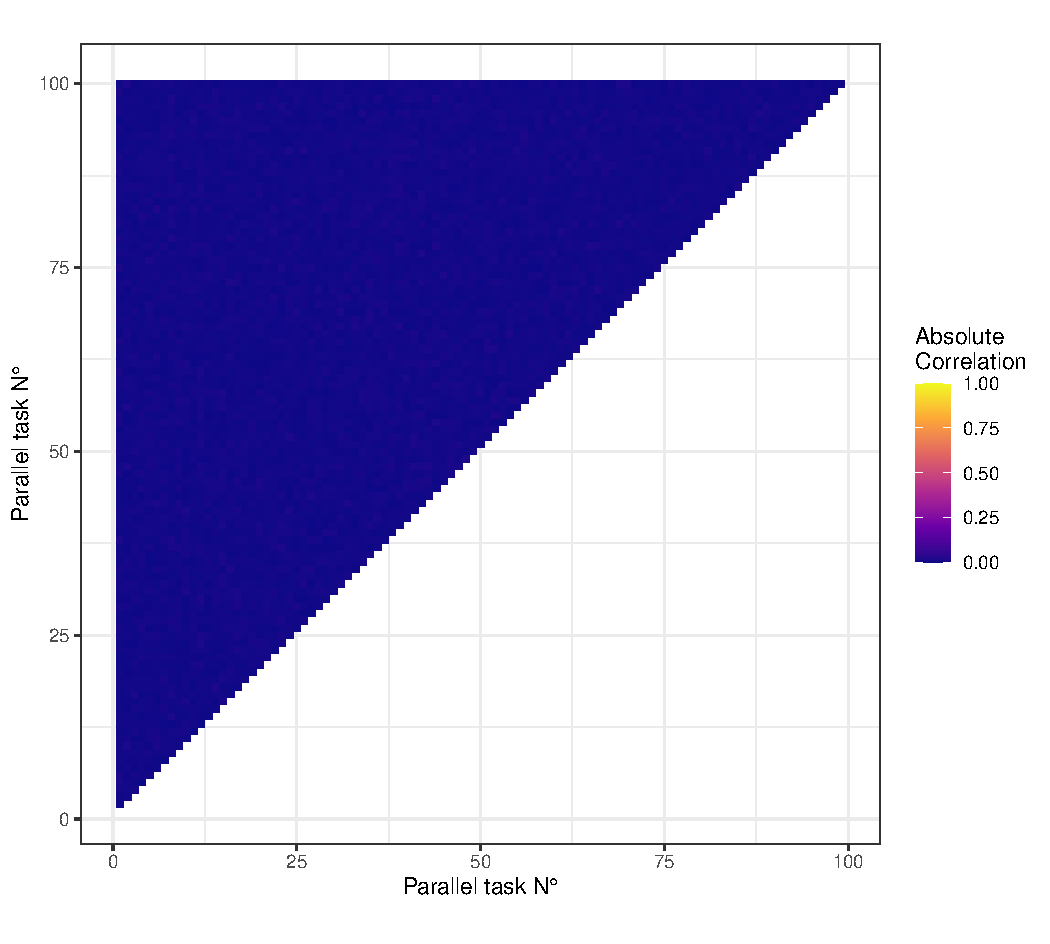
\includegraphics[width=\linewidth,height=0.3\textheight,keepaspectratio]{../../outputs/diagnostics/error_dependence.pdf}

}

\end{figure}%

\begin{figure}

\caption{\label{fig-diag-errors-distribution}Random errors -
Distribution}

\centering{

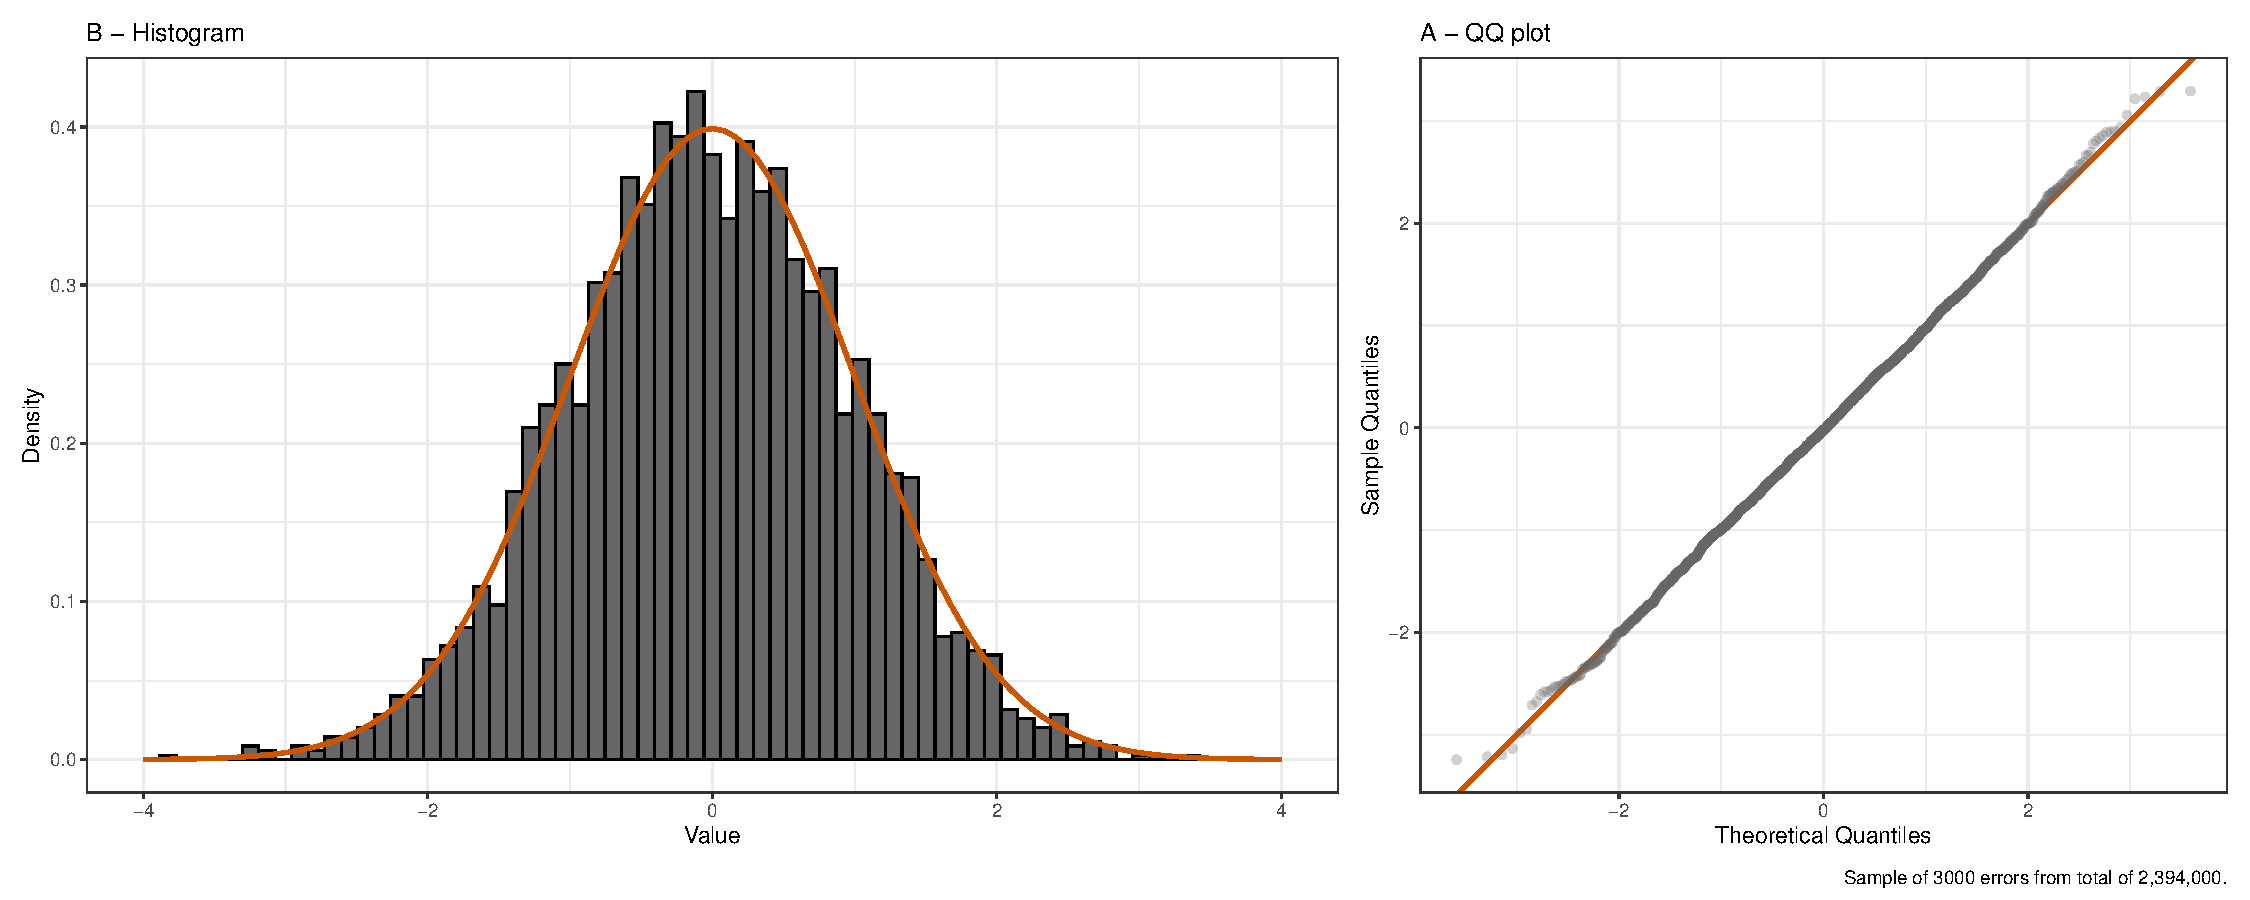
\includegraphics[width=\linewidth,height=0.3\textheight,keepaspectratio]{../../outputs/diagnostics/error_distribution.pdf}

}

\end{figure}%

\subsection{Estimated errors}\label{sec-app-diag-error}

The Figure~\ref{fig-residuals_distribution} presents the distribution of
the estimation errors (residuals) across models, while
Figure~\ref{fig-forecast_errors_distribution} shows the distribution of
forecasting errors. Overall, the distributions align with expectations,
with the former exhibiting fatter tails than the latter. In the former,
approximately 10,000 observations fall outside the range of the x-axis,
some of which were identified as outliers.

\begin{figure}

\caption{\label{fig-residuals_distribution}Residuals - Distribution}

\centering{

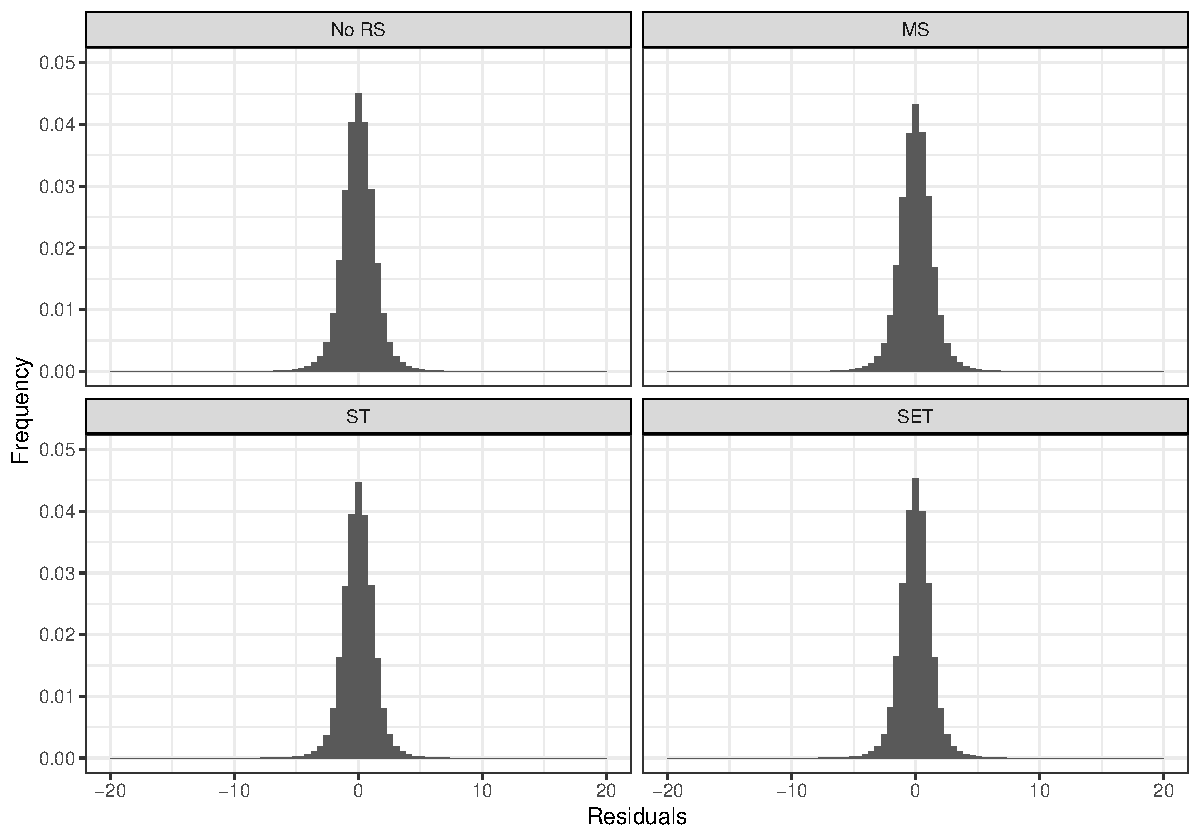
\includegraphics[width=\linewidth,height=0.35\textheight,keepaspectratio]{../../outputs/diagnostics/residuals_distribution.pdf}

}

\end{figure}%

\begin{figure}

\caption{\label{fig-forecast_errors_distribution}Forecasting errors -
Distribution}

\centering{

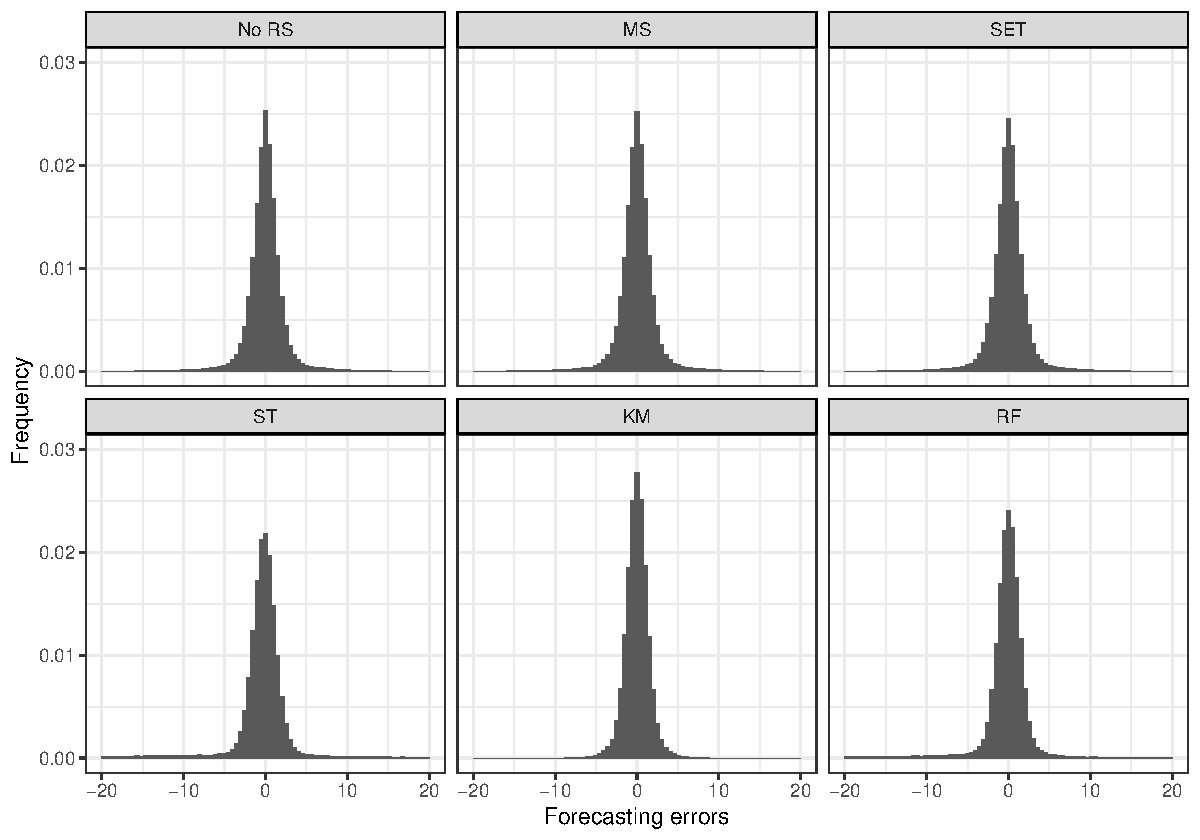
\includegraphics[width=\linewidth,height=0.35\textheight,keepaspectratio]{../../outputs/diagnostics/forecast_errors_distribution.pdf}

}

\end{figure}%

\subsection{Regime proportions}\label{sec-app-diag-r}

The Figure~\ref{fig-regimes_est} illustrates the distribution of the
proportion of the least frequent estimated regime, separated by model.
Estimations below the dashed line had only two observations in the
regime and were excluded.

\begin{figure}

\caption{\label{fig-regimes_est}Regime proportion - Distribution}

\centering{

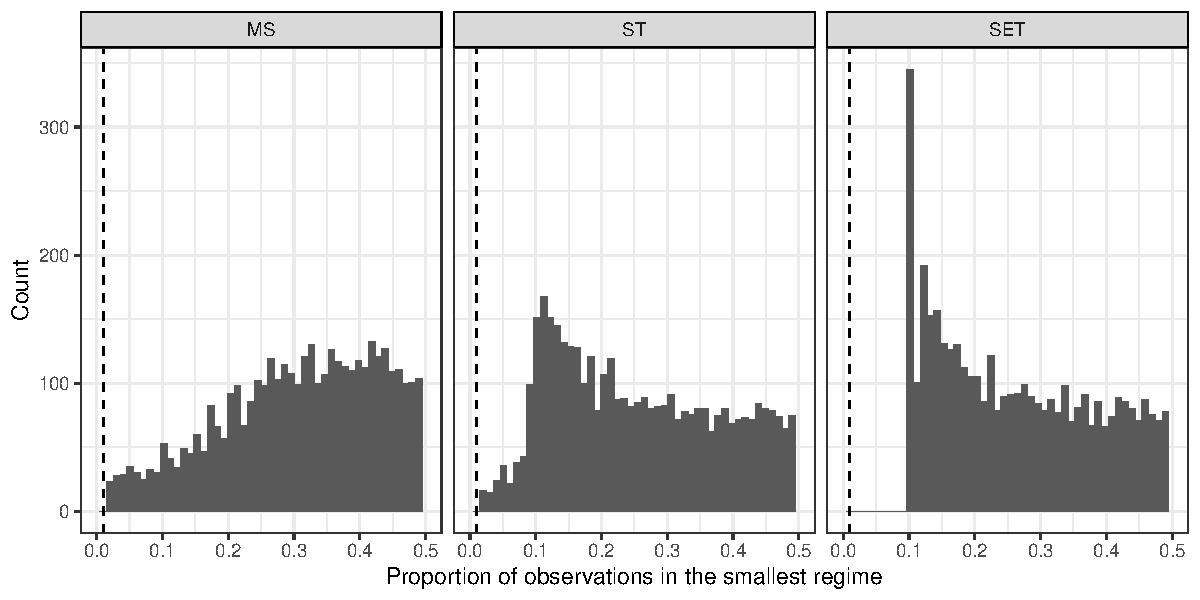
\includegraphics[width=\linewidth,height=0.25\textheight,keepaspectratio]{../../outputs/diagnostics/regimes_est.pdf}

}

\end{figure}%

\subsection{Parameters and model metadata}\label{sec-app-diag-params}

The Figure~\ref{fig-parameters_distribution} visualizes the distribution
of the estimated parameters across models and parameters. All by-regime
values of a parameter are grouped together in the same panel. Overall,
the distributions align with expectations, with approximately 10,000
values falling outside the range of the x-axis, some of which were
identified as outliers.

The Figure~\ref{fig-metadata_distribution} displays the distribution of
RGP-related metadata, such as the MS transition probabilities, ST
\(\gamma\), and \(SET\) \(\tau\). Overall, the distributions align with
expectations.

The Table~\ref{tbl-coefs_table} compares the model parameters to the
true values of the DGPs. Each group of rows corresponds to the moments
of a DGP. The first two columns relate to the values conditional on
regimes 1 and 2, while the third column provides the unconditional
values. Each cell contains the moment value, with the p-value of the
null hypothesis that the moment equals its true value in brackets. The
table includes only symmetric RGPs and large SGPs. Note that the moments
do not need to match exactly, as all models allow for parameter
variation, which differs from the assumptions about regime natures.

\begin{figure}

\caption{\label{fig-parameters_distribution}Parameters - Distribution}

\centering{

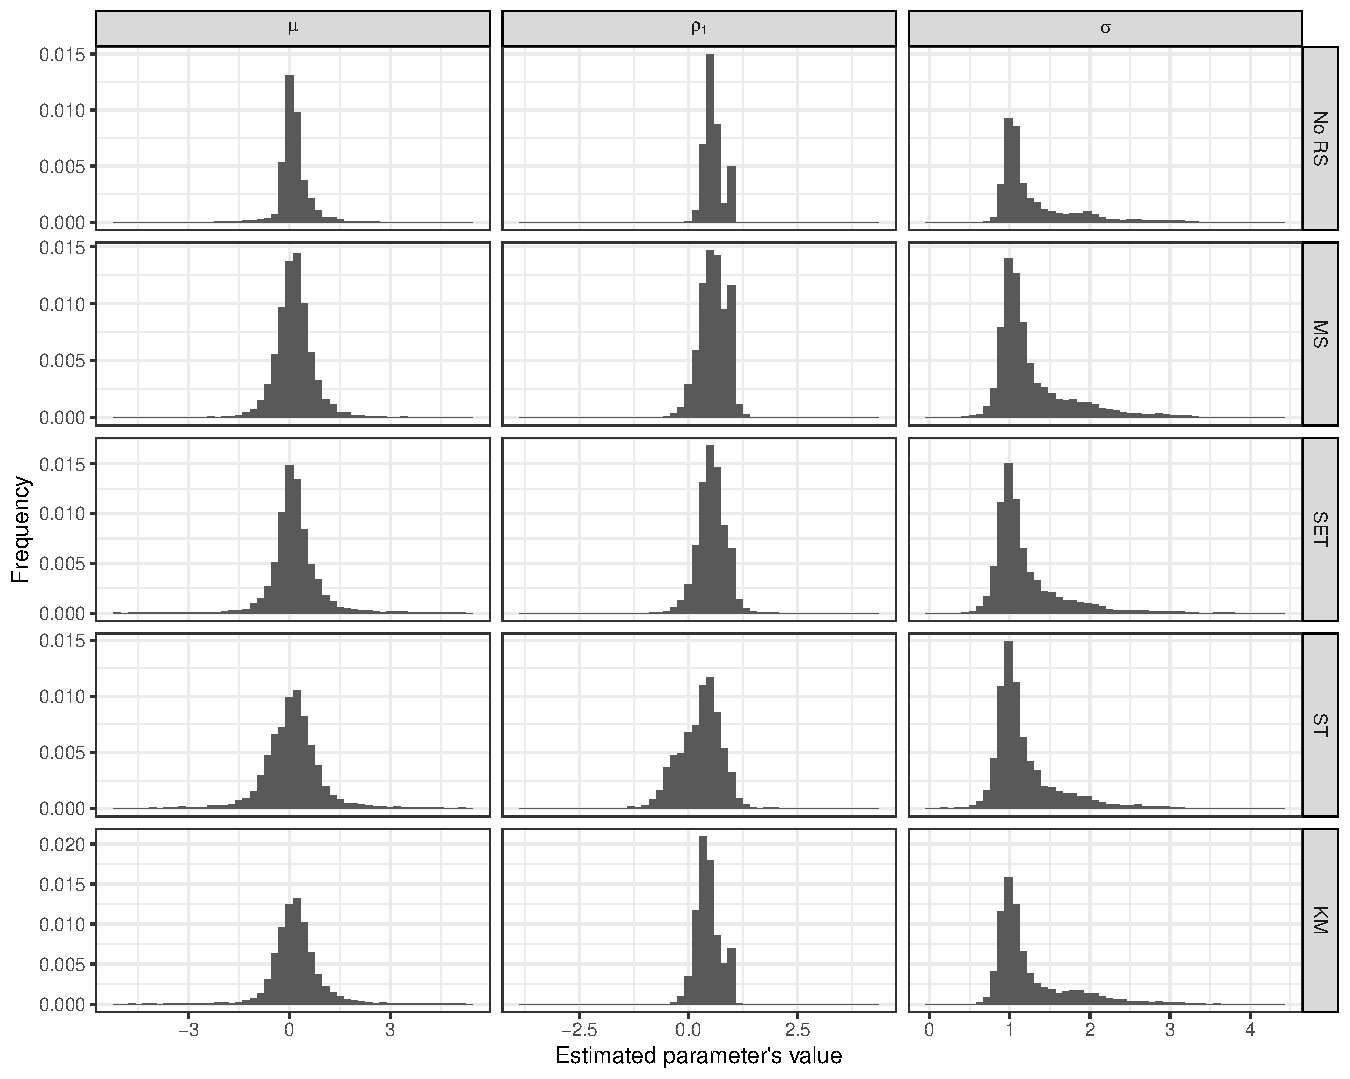
\includegraphics[width=\linewidth,height=0.45\textheight,keepaspectratio]{../../outputs/diagnostics/parameters_distribution.pdf}

}

\end{figure}%

\begin{figure}

\caption{\label{fig-metadata_distribution}Model metadata - Distribution}

\centering{

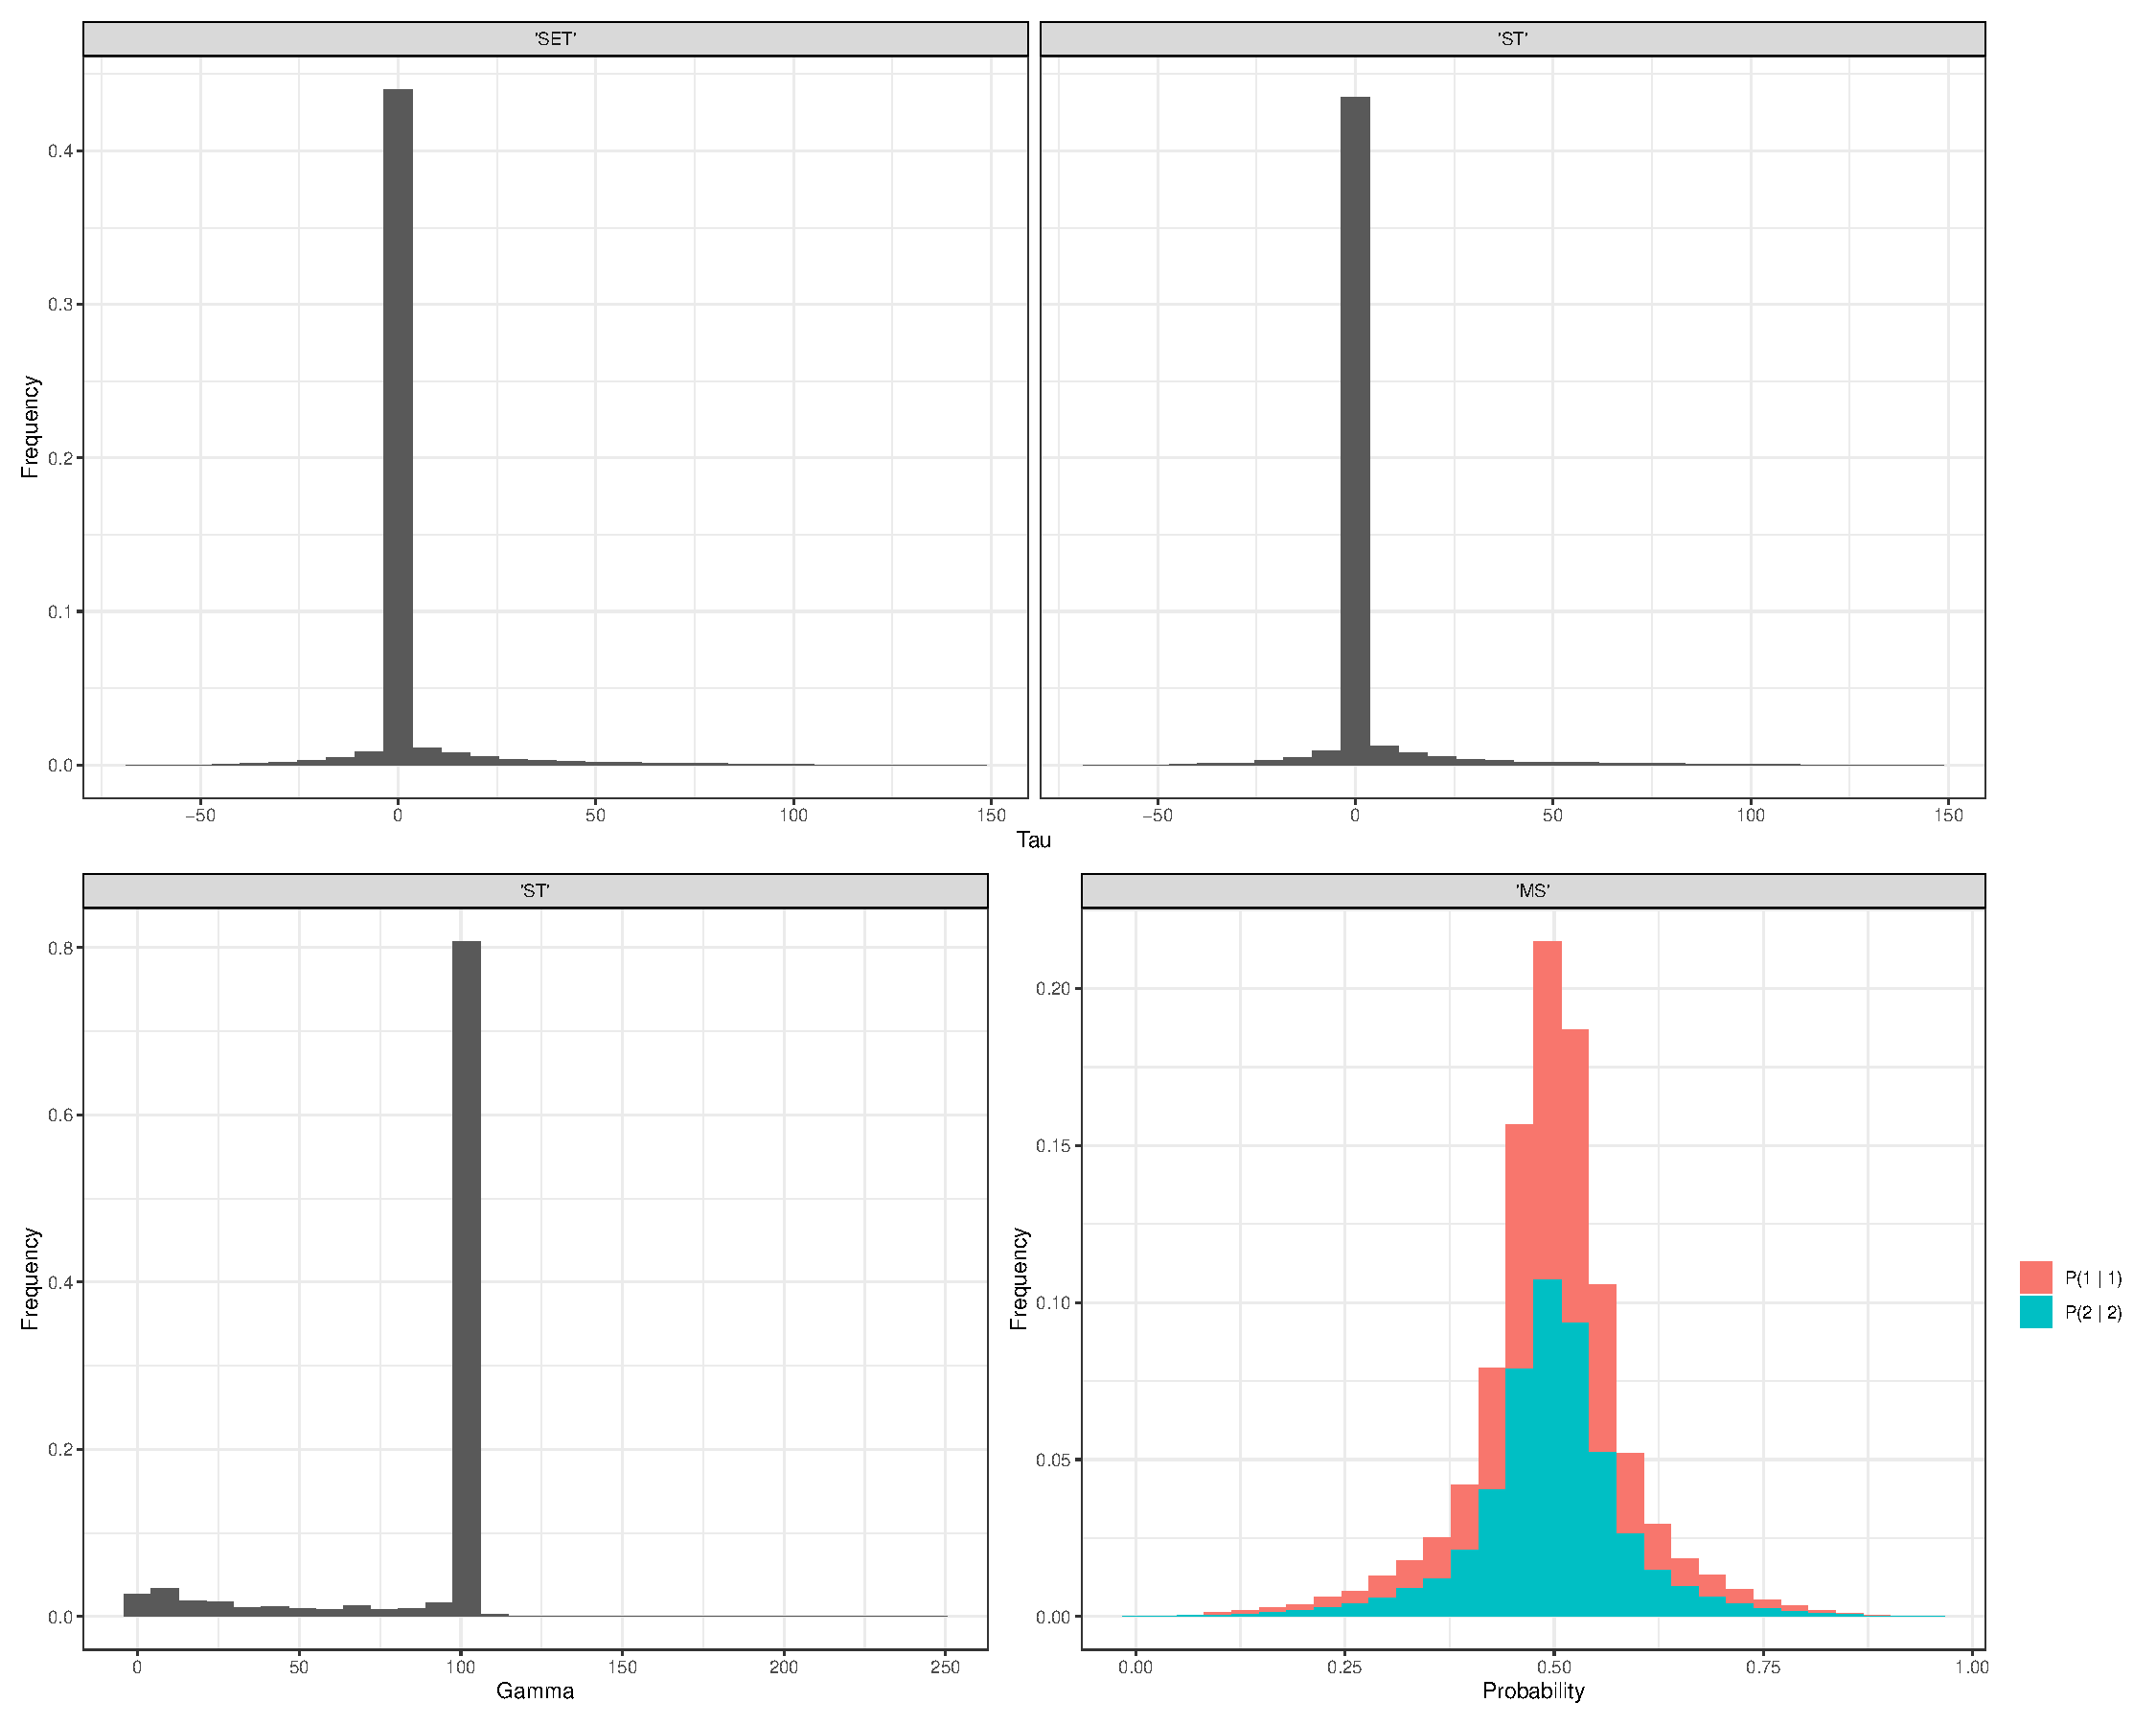
\includegraphics[width=\linewidth,height=0.35\textheight,keepaspectratio]{../../outputs/diagnostics/metadata_distribution.pdf}

}

\end{figure}%

\subsection{Metrics calculation}\label{sec-app-diag-metrics}

The calculated metrics are presented in Table~\ref{tbl-metrics_table}.
Each group of rows corresponds to the moments of a DGP. The first two
columns relate to the values conditional on regimes 1 and 2, while the
third column provides the unconditional values. Each cell contains the
moment value, with the p-value of the null hypothesis that the moment
equals its true value in brackets. The table includes only symmetric
RGPs and large SGPs. Note that the moments do not need to match exactly,
as all models allow for parameter variation, which differs from the
assumptions about regime natures.

\begin{landscape}

\begin{table}

\caption{\label{tbl-i_independence}RMSE and simulation index
relationship}

\centering{

\begin{tabular}{@{\extracolsep{5pt}}lc} 
\\[-1.8ex]\hline 
\hline \\[-1.8ex] 
\\[-1.8ex] & RMSE \\ 
\hline \\[-1.8ex] 
 $i$ & $-$0.346 (4.293) \\ 
  $i^2$ & 1.578 (2.036) \\ 
  $i^3$ & 0.553 (1.444) \\ 
  $\log(i)$ & 0.004 (0.014) \\ 
  Constant & 1.284$^{***}$ (0.073) \\ 
 \hline \\[-1.8ex] 
Observations & 123,137 \\ 
R$^{2}$ & 0.00002 \\ 
Adjusted R$^{2}$ & $-$0.00001 \\ 
Residual Std. Error & 1.026 \\ 
F Statistic p-value & 0.622 \\ 
\hline 
\hline \\[-1.8ex] 
\textit{Note:}  & \multicolumn{1}{r}{$^{*}$p$<$0.1; $^{**}$p$<$0.05; $^{***}$p$<$0.01} \\ 
\end{tabular} 


}

\end{table}%

\begin{table}[!htbp]

\caption{\label{tbl-coefs_table}Estimated coefficients across DGPs}

\centering{

\begin{table}[t]
\fontsize{12.0pt}{14.0pt}\selectfont
\begin{tabular*}{\linewidth}{@{\extracolsep{\fill}}l|l|llllll}
\toprule
\multicolumn{2}{l}{} & \multicolumn{2}{c}{{\(\mu^s\)}} & \multicolumn{2}{c}{{\(\rho^s_1\)}} & \multicolumn{2}{c}{{\(\sigma^s\)}} \\ 
\cmidrule(lr){3-4} \cmidrule(lr){5-6} \cmidrule(lr){7-8}
RGP & RN & \(s = 1\) & \(s = 2\) & \(s = 1\) & \(s = 2\) & \(s = 1\) & \(s = 2\) \\ 
\midrule\addlinespace[2.5pt]
MS, \(p_{21} = 0.1\) & \(\mu ~ (0, 1)\) & .17 (.012)*** & .61 (.015)*** & .67 (.008)*** & .57 (.008)*** & 1.07 (.007)*** & 1.08 (.007)*** \\ 
 & \(\rho_{1} ~ (0.4, 0.6)\) & -.01 (.012) & .02 (.012) & .33 (.011)*** & .75 (.008)*** & 1.02 (.007)*** & 1.06 (.006)*** \\ 
 & \(\sigma ~ (1, 2)\) & .01 (.017) & -.01 (.017) & .46 (.015)*** & .5 (.015) & 1.42 (.011)*** & 1.7 (.013)*** \\ 
SET, \(\tau = 0.5\) & \(\mu ~ (0, 1)\) & .22 (.018)*** & 1.11 (.028)*** & .74 (.01)*** & .5 (.014) & .98 (.006)*** & .97 (.006)*** \\ 
 & \(\rho_{1} ~ (0.4, 0.6)\) & .29 (.018)*** & .04 (.021)* & .36 (.01)*** & .77 (.009)*** & .97 (.006)*** & .96 (.005)*** \\ 
 & \(\sigma ~ (1, 2)\) & -.05 (.023)* & .02 (.024) & .47 (.014)** & .5 (.013) & 1.19 (.008)*** & 1.46 (.009)*** \\ 
ST, \(\tau = 0.5\) & \(\mu ~ (0, 1)\) & -.19 (.027)*** & .77 (.017)*** & .17 (.021)*** & .11 (.02)*** & .97 (.006)*** & .95 (.006)*** \\ 
 & \(\rho_{1} ~ (0.4, 0.6)\) & -.13 (.032)*** & .04 (.022) & -.35 (.018)*** & .71 (.01)*** & .97 (.005)*** & .96 (.006)*** \\ 
 & \(\sigma ~ (1, 2)\) & -.08 (.057) & .01 (.058) & .25 (.023)*** & .26 (.023)*** & 1.38 (.009)*** & 1.64 (.009)*** \\ 
\bottomrule
\end{tabular*}
\end{table}



}

\end{table}%

\begin{table}[!htbp]

\caption{\label{tbl-metrics_table}Estimated metrics across DGPs}

\centering{

\begin{table}[t]
\fontsize{12.0pt}{14.0pt}\selectfont
\begin{tabular*}{\linewidth}{@{\extracolsep{\fill}}l|l|lllllllll}
\toprule
\multicolumn{2}{l}{} & \multicolumn{3}{c}{{\(\hat{\mu}(. | s)\)}} & \multicolumn{3}{c}{{\(\hat{\rho}_1(. | s)\)}} & \multicolumn{3}{c}{{\(\hat{\sigma}(. | s)\)}} \\ 
\cmidrule(lr){3-5} \cmidrule(lr){6-8} \cmidrule(lr){9-11}
RGP & RN & \(s = 1\) & \(s = 2\) & \(⊥ ~ s\) & \(s = 1\) & \(s = 2\) & \(⊥ ~ s\) & \(s = 1\) & \(s = 2\) & \(⊥ ~ s\) \\ 
\midrule\addlinespace[2.5pt]
MS, \(p_{21} = 0.1\) & \(\mu ~ (0, 1)\) & .22 (.013)*** & 1.78 (.012)*** & 1.04 (.016) & .38 (.005)*** & .38 (.005)*** & .55 (.002) & 1.17 (.007)** & 1.18 (.006)*** & 1.4 (.006) \\ 
 & \(\rho_{1} ~ (0.4, 0.6)\) & .01 (.008) & .01 (.022) & .01 (.013) & .15 (.006)*** & .57 (.004)*** & .51 (.004) & 1.01 (.005) & 1.47 (.011)*** & 1.3 (.008) \\ 
 & \(\sigma ~ (1, 2)\) & 0 (.013) & 0 (.021) & 0 (.013) & .38 (.006)*** & .38 (.005)*** & .44 (.003) & 1.2 (.007)*** & 2.22 (.012)*** & 1.81 (.011) \\ 
SET, \(\tau = 0.5\) & \(\mu ~ (0, 1)\) & -.19 (.014)*** & 2.07 (.009)*** & 1.47 (.016) & .2 (.008)*** & .37 (.004)*** & .6 (.002) & 1.05 (.007)*** & 1.11 (.005)*** & 1.47 (.008) \\ 
 & \(\rho_{1} ~ (0.4, 0.6)\) & -.08 (.007)*** & 1.29 (.014)*** & .63 (.013) & .08 (.006)*** & .39 (.006)*** & .54 (.003) & 1 (.005)*** & 1.2 (.007)*** & 1.3 (.007) \\ 
 & \(\sigma ~ (1, 2)\) & -.43 (.007)*** & .85 (.02)*** & -.01 (.012) & .19 (.005)*** & .17 (.007)*** & .44 (.003) & 1.1 (.004)*** & 2.06 (.012)*** & 1.59 (.009) \\ 
ST, \(\tau = 0.5\) & \(\mu ~ (0, 1)\) & 1.02 (.006)*** & .56 (.008)*** & .85 (.006) & .12 (.005)*** & .04 (.007)*** & .27 (.004) & 1.04 (.004)*** & 1.01 (.005)*** & 1.05 (.003) \\ 
 & \(\rho_{1} ~ (0.4, 0.6)\) & .41 (.009)*** & -.66 (.011)*** & -.39 (.011) & -.01 (.008)*** & .45 (.005)*** & .53 (.003) & 1 (.006)*** & 1.23 (.007)*** & 1.27 (.007) \\ 
 & \(\sigma ~ (1, 2)\) & .81 (.01)*** & -.58 (.013)*** & 0 (.013) & .1 (.006)*** & .24 (.005)*** & .44 (.003) & 1.33 (.006)*** & 1.89 (.009)*** & 1.81 (.007) \\ 
\bottomrule
\end{tabular*}
\end{table}



}

\end{table}%

\end{landscape}




\end{document}
